%\documentclass[onecolumn]{IEEEtranTIE}
\documentclass[journal]{IEEEtranTIE}
\usepackage{graphicx}
\usepackage{cite}
\usepackage{picinpar}
\usepackage{amsmath}
\usepackage{url}
\usepackage{flushend}
\usepackage[latin1]{inputenc}
\usepackage{colortbl}
\usepackage{soul}
\usepackage{multirow}
\usepackage{pifont}
\usepackage{color}
\usepackage{alltt}
\usepackage[hidelinks]{hyperref}
\usepackage{enumerate}
\usepackage{siunitx}
\usepackage{breakurl}
\usepackage{epstopdf}
\usepackage{pbox}
% Added
\usepackage{amssymb}
\usepackage{amsthm}
\usepackage[table]{xcolor}
\newtheorem{theorem}{Theorem}
\newtheorem{lemma}{Lemma}
\newtheorem{remark}{Remark}
\newtheorem{definition}{Definition}
\newtheorem{assumption}{Assumption}
\usepackage[ruled,vlined,linesnumbered]{algorithm2e}
\usepackage{subfigure}
%\usepackage{algorithmic}
%\definecolor{lightgray}{gray}{0.9}
\definecolor{lightgray}{rgb}{0.97,0.97,0.97}


% some macros for symbols from Christoph
%	Define new math operators
\DeclareMathOperator*{\imag}{im}
\DeclareMathOperator*{\kernel}{kern} 
\DeclareMathOperator*{\image}{imag} 
\DeclareMathOperator*{\essinf}{ess-inf}
\DeclareMathOperator*{\esssup}{ess-sup}
\DeclareMathOperator*{\dist}{dist}
\DeclareMathOperator*{\diag}{diag}
\DeclareMathOperator*{\blockdiag}{blockdiag}
\DeclareMathOperator*{\graph}{graph}
\DeclareMathOperator*{\sign}{sign}
\DeclareMathOperator*{\rank}{rank}
\DeclareMathOperator*{\sat}{sat}
\DeclareMathOperator*{\satvec}{\textbf{sat}}
\DeclareMathOperator*{\spec}{spec}
\DeclareMathOperator*{\loc}{loc}
\DeclareMathOperator*{\grad}{grad}
\DeclareMathOperator*{\fin}{fin}
\ifx \chosenClassCompatibility\classieeeojiesCompatiblity
    % \vol command already defined in file ieeeojies.cls --> ignore math operator \vol
\else % default
    \DeclareMathOperator*{\vol}{vol}
\fi
\DeclareMathOperator*{\col}{col}
\DeclareMathOperator*{\row}{row}
\DeclareMathOperator*{\lin}{lin}
\DeclareMathOperator*{\step}{step}
\DeclareMathOperator*{\arctanTWO}{arctan2}
\DeclareMathOperator*{\atanTWO}{arctan2}
\DeclareMathOperator*{\argmin}{arg\,min}
\DeclareMathOperator*{\argmax}{arg\,max}
\DeclareMathOperator*{\floor}{floor}
\DeclareMathOperator*{\ceil}{ceil}
\DeclareMathOperator*{\movmean}{movmean}
\DeclareMathOperator*{\mean}{mean}

% pulse minus with paranthesis
\def\plusMINUS{\substack{(+)\\[-0.25ex]-}}
\def\PLUSminus{\substack{+\\[-0.25ex](-)}}


%	Abbreviate sets, compact sets  (of numbers, ...)
\newcommand*{\N}{\mathbb{N}}
\newcommand*{\B}{\mathbb{B}}
\newcommand*{\Z}{\mathbb{Z}}
\newcommand*{\Q}{\mathbb{Q}}
\newcommand*{\R}{\mathbb{R}}
\newcommand*{\Rzp}{\mathbb{R}_{\geq 0}}
\newcommand*{\Rp}{\mathbb{R}_{> 0}}
\newcommand*{\Rn}{\mathbb{R}_{< 0}}
\newcommand*{\C}{\mathbb{C}}
\newcommand*{\Cn}{\mathbb{C}_{< 0}}
\newcommand*{\Cp}{\mathbb{C}_{< 0}}
\newcommand*{\Czp}{\mathbb{C}_{\geq 0}}
%	compact set
\newcommand*{\cset}[1]{\mathfrak{#1}}
%	open set
\newcommand*{\oset}[1]{\mathcal{#1}}
%	function set
\newcommand*{\fset}[1]{\mathcal{#1}}
%	operator class 
\newcommand*{\oclass}[1]{\mathcal{#1}}
%	boundary set
\newcommand*{\bset}[1]{\mathcal{#1}}

% set definition
\newcommand*{\setdef}[2]{\left\{\ #1\ \left|\vphantom{#1}\ #2\ \right.\right\}}
% interval where system is in steady-state
\newcommand*{\Iss}{\mathbb{I}_{\mathrm{ss}}}

%	function spaces
\newcommand*{\Lp}[1]{\fset{L}^{#1}}
\newcommand*{\Lk}[1]{\fset{L}^{#1}}
\newcommand*{\Lploc}[1]{\fset{L}^{#1}_{\loc}}
\newcommand*{\Lkloc}[1]{\fset{L}^{#1}_{\loc}}
\newcommand*{\Lone}{\fset{L}^{1}}
\newcommand*{\Loneloc}{\fset{L}^{1}_{\loc}}
\newcommand*{\Ltwo}{\fset{L}^{2}}
\newcommand*{\Linf}{\fset{L}^{\infty}}
\newcommand*{\Linfloc}{\fset{L}^{\infty}_{\loc}}
\newcommand*{\Ck}[1]{\fset{C}^{#1}}
\newcommand*{\Czero}{\fset{C}}
\newcommand*{\Cuni}{\fset{C}^{\rm uni}}
\newcommand*{\Cabs}{\fset{C}^{\rm abs}}
\newcommand*{\Cabsloc}{\fset{C}^{\rm abs}_{\loc}}
\newcommand*{\Cpw}{\fset{C}^{\rm pw}}
\newcommand*{\CLip}{\fset{C}^{\rm L}}
\newcommand*{\CLiploc}{\fset{C}^{\rm L}_{\loc}}
\newcommand*{\Cone}{\fset{C}^{1}}
\newcommand*{\Ctwo}{\fset{C}^{2}}
\newcommand*{\Cinf}{\fset{C}^{\infty}}
\newcommand*{\Wkinf}[1]{\fset{W}^{#1,\infty}}
\newcommand*{\Woneinf}{\fset{W}^{1,\infty}}
\newcommand*{\Wtwoinf}{\fset{W}^{2,\infty}}

%	norm ||.||
\newcommand*{\norm}[1]{\lVert #1 \rVert}
\newcommand*{\normscaled}[1]{\left\lVert #1 \right\rVert}
% ||.||_infty
\newcommand*{\esnorm}[1]{\lVert #1 \rVert_{\infty}}
\newcommand*{\Wnorm}[3]{\lVert #3 \rVert_{#1,#2}}
\newcommand*{\Lnorm}[2]{\lVert #2 \rVert_{\fset{L}^{#1}}}
\newcommand*{\Lpnorm}[2]{\lVert #2 \rVert_{\fset{L}^{#1}}}
\newcommand*{\Lpnormscaled}[2]{\left\| #2 \right\|_{\fset{L}^{#1}}}

%	limits
\newcommand*{\limtoinfty}[1]{\lim_{#1 \to \infty}}
\newcommand*{\limtozero}[1]{\lim_{#1 \to 0}}
\newcommand*{\limto}[2]{\lim_{#1 \to #2}}

% 	Lapace
\newcommand*{\laplaceT}[1]{\mathscr{L}\left\{#1\right\}}
\newcommand*{\laplaceIT}[1]{\mathscr{L}^{-1}\left\{#1\right\}}

%	myVector = \mv
\newcommand*{\mv}[1]{\boldsymbol{#1}}
%	myMatrix = \mm
\newcommand*{\mm}[1]{\boldsymbol{#1}}
%	myOperator = \mo
\newcommand*{\mo}[1]{\boldsymbol{\mathfrak{#1}}}
%	inner product <.,.>
\newcommand*{\iproduct}[2]{\langle #1,\, #2 \rangle}

%	Units
\newcommand*{\Ohm}{\Omega}

%	Differentiation
%	[<1> = number/order of derivative], <2> = with respect to what, 
\newcommand*{\fdiff}[2]{\frac{\mathrm{d}^{#1}}{\mathrm{d}{#2}^{#1}}\,}
\newcommand*{\fdiffsmall}[2]{\tfrac{\mathrm{d}^{#1}}{\mathrm{d}{#2}^{#1}}\,}
\newcommand*{\fdiffs}[3]{\dfrac{\mathrm{d}^{#1}{#3}}{\mathrm{d} {#2}^{#1}}}
\newcommand*{\fdiffssmall}[3]{\tfrac{\mathrm{d}^{#1}{#3}}{\mathrm{d} {#2}^{#1}}}
\newcommand*{\fpartial}[2]{\frac{\partial^{#1}}{\partial #2^{#1}}\,}
\newcommand*{\fpartialsmall}[2]{\frac{\partial^{#1}}{\partial #2^{#1}}\,}
\newcommand*{\fpartials}[3]{\dfrac{\partial^{#1}{#3}}{\partial {#2}^{#1}}}
\newcommand*{\fpartialssmall}[3]{\tfrac{\partial^{#1}{#3}}{\partial {#2}^{#1}}}
%	<1> = function to be differentiated, <2> = with respect to what, [<3> = number/order of derivative]
\newcommand*{\fdiffcom}[2]{\tfrac{\mathrm{d} #1}{\mathrm{d}{#2}}}
\newcommand*{\fdiffhocom}[3]{\dfrac{\mathrm{d}^{#3}#1}{\mathrm{d}{#2}^{#3}}}
\newcommand*{\fpartialcom}[2]{\tfrac{\partial #1}{\partial #2}}
\newcommand*{\fpartialhocom}[3]{\tfrac{\partial^{#3}#1}{\partial #2^{#3}}}
% %	[<1> = number/order of derivative], <2> = with respect to what, 
\newcommand*{\dfdx}[2]{\frac{\mathrm{d}#1}{\mathrm{d}#2}}
\newcommand*{\dfdxsmall}[2]{\tfrac{\mathrm{d}#1}{\mathrm{d}#2}}
\newcommand*{\dfndxn}[3]{\tfrac{\mathrm{d}^{#3}{#1}}{\mathrm{d}#2^{#3}}}
% %	<1> = function to be differentiated, <2> = with respect to what, [<3> = number/order of derivative]
\newcommand*{\fdiffhosmall}[3]{\tfrac{\mathrm{d}^{#3} #1}{\mathrm{d}{#2}^{#3}}}
\newcommand*{\pfpx}[2]{\tfrac{\partial#1}{\partial#2}}
\newcommand*{\pfpxpy}[3]{\tfrac{\partial^2#1}{\partial#2\,\partial#3}}
\newcommand*{\pfnpxn}[3]{\tfrac{\partial^{#3}{#1}}{\partial#2^{#3}}}
% derivatives with respect to t
\newcommand*{\dt}{\mathrm{d}t}
\newcommand*{\ddt}{\tfrac{\mathrm{d}}{\mathrm{d}t}}
\newcommand*{\ppt}{\tfrac{\partial}{\partial t}}
\newcommand*{\ddtsmall}{\tfrac{\mathrm{d}}{\mathrm{d}t}}
\newcommand*{\dddt}{\tfrac{\mathrm{d}^2}{\mathrm{d}t^2}}
\newcommand*{\pppt}{\tfrac{\partial^2}{\partial t^2}}
\newcommand*{\dddtsmall}{\tfrac{\mathrm{d}^2}{\mathrm{d}t^2}}
\newcommand*{\dtau}{\dx{\tau}}
\newcommand*{\dx}[1]{\mathrm{\, d} #1 \,}
\newcommand*{\musteq}{\stackrel{!}{=}}

% derivatives with respect to x
\newcommand*{\ddx}{\tfrac{\mathrm{d}}{\mathrm{d}x}}
\newcommand*{\ppx}{\tfrac{\partial}{\partial x}}
\newcommand*{\ddxsmall}{\tfrac{\mathrm{d}}{\mathrm{d}x}}
\newcommand*{\pppx}{\tfrac{\partial^2}{\partial x^2}}
\newcommand*{\dddx}{\tfrac{\mathrm{d}^2}{\mathrm{d}x^2}}
\newcommand*{\dddxsmall}{\tfrac{\mathrm{d}^2}{\mathrm{d}x^2}}

% misc
\DeclareMathOperator*{\eqforce}{\stackrel{!}{=}}
\newcommand*{\abs}[1]{|#1|}
\newcommand*{\absscaled}[1]{\left| #1 \right|}
\newcommand*{\trans}[1]{#1^{\top}}
\newcommand*{\inv}[1]{#1^{-1}}
\newcommand*{\I}{\oset{I}}
\newcommand*{\D}{\oset{D}}
\newcommand*{\conj}[1]{#1^*}
\newcommand*{\hermconj}[1]{#1^{\mathsf{H}}}

% normalization
\newcommand*{\normalized}[1]{\big[#1\big]_{\!\mathrm{p.u.}}}
% ----------------------------------------------------------------------------------
% IDENTICAL DEFINITIONS for ENGLISH and GERMAN - START
% ----------------------------------------------------------------------------------
% control
\newcommand*{\DEZIBEL}{\protect\mathrm{dB}}
\newcommand*{\MYREF}{\mathrm{ref}}			% reference / Referenz 	
\newcommand*{\PROPORTIONAL}{\mathrm{p}}		% proportional	
\newcommand*{\INTEGRATOR}{\mathrm{i}}		% integral / integrierend
\newcommand*{\DERIVATIVE}{\mathrm{d}}		% differential / differenzierend
\newcommand*{\INTERNALMODEL}{\mathrm{im}}	% internal model / internes Model
\newcommand*{\ANTIWINDUP}{\mathrm{aw}}		% anti-windup
\newcommand*{\SYSTEMSUB}{\mathrm{s}}		% system / System
\newcommand*{\SYSTEM}{\mathrm{S}}			% system / System
\newcommand*{\PICON}{\mathrm{pi}}			
\newcommand*{\FCCON}{\mathrm{fc}}
\newcommand*{\MEASURED}{\mathrm{m}}			% measured / (ge)messen
% three phase systems 
\newcommand*{\dAXIS}{d}
\newcommand*{\qAXIS}{q}
\newcommand*{\zeroAXIS}{0}
\newcommand*{\gammaAXIS}{\gamma}
\newcommand*{\arAXIS}{a_{\mathrm{r}}}
\newcommand*{\brAXIS}{b_{\mathrm{r}}}
\newcommand*{\crAXIS}{c_{\mathrm{r}}}
\newcommand*{\alphaAXIS}{\alpha}
\newcommand*{\betaAXIS}{\beta}
\newcommand*{\kCOSY}{\dAXIS\qAXIS\gammaAXIS}            % [DEPRECATED]
\newcommand*{\dqgaCOSY}{\dAXIS\qAXIS\gammaAXIS}
\newcommand*{\dqCOSY}{\dAXIS\qAXIS} 			
\newcommand*{\sCOSY}{\alphaAXIS\betaAXIS\gammaAXIS}     % [DEPRECATED]
\newcommand*{\albegaCOSY}{\alphaAXIS\betaAXIS\gammaAXIS}
\newcommand*{\alphabetaCOSY}{\alphaAXIS\betaAXIS}       % [DEPRECATED]
\newcommand*{\albeCOSY}{\alphaAXIS\betaAXIS}
\newcommand*{\abcCOSY}{abc}
\newcommand*{\uvwCOSY}{uvw}
\newcommand*{\arbrcrCOSY}{a_{\mathrm{r}}b_{\mathrm{r}}c_{\mathrm{r}}}
\newcommand*{\AtoB}{a\text{-}b}
\newcommand*{\BtoA}{b\text{-}a}
\newcommand*{\BtoC}{b\text{-}c}
\newcommand*{\CtoB}{c\text{-}b}
\newcommand*{\CtoA}{c\text{-}a}
\newcommand*{\AtoC}{a\text{-}c}
\newcommand*{\LTL}{a\text{-}b\text{-}c}
\newcommand*{\PARK}{\mathrm{p}}
\newcommand*{\CLARKE}{\mathrm{c}}	
\newcommand*{\PHASE}{p}						% phase / Phase
% electrical signals: voltages, currents, flux linkage, etc
\newcommand*{\VOLTAGE}{u} 					% voltage (e.g. $u$ or $v$)
\newcommand*{\CURRENT}{i}					% current
\newcommand*{\FLUX}{\psi} 					% flux (e.g. $\psi$ or $\lambda$)
\newcommand*{\TORQUE}{m} 					% torque (e.g. $m$ or $\tau$); attention: note that $\tau$ has conflict with time 
\newcommand*{\TEMPERATURE}{\vartheta} 		% temperature (e.g. temperature of stator and rotor)
% power electronics
\newcommand*{\INTERLOCK}{\mathrm{itl}}		% interlock time
\newcommand*{\BTB}{\mathrm{btb}}			% back-to-back (converter)
\newcommand*{\SWITCH}{s} 					% switch / Schalter (e.g. $s$ or $\sigma$); attentation: note that $\sigma$ has conflict with Heaviside function
% electrical drives
\newcommand*{\PM}{\mathrm{pm}}				% permanent magnet / Permanentmagnet
\newcommand*{\EE}{\mathrm{ee}}				% electrical excitation / elektrische Erregung
\newcommand*{\SE}{\mathrm{se}}
\newcommand*{\MACHINE}{\mathrm{m}}
\newcommand*{\GENERATOR}{\mathrm{g}}
\newcommand*{\MECH}{\mathrm{m}}
\newcommand*{\STATOR}{\mathrm{s}}
\newcommand*{\ROTOR}{\mathrm{r}}
\newcommand*{\EXCITATION}{\mathrm{e}}
\newcommand*{\ELEC}{\mathrm{el}}
\newcommand*{\ANKER}{\mathrm{a}}
\newcommand*{\alpharAXIS}{\alpha_{\ROTOR}}
\newcommand*{\betarAXIS}{\beta_{\ROTOR}}
\newcommand*{\gammarAXIS}{\gamma_{\mathrm{r}}}
\newcommand*{\rCOSY}{\alpharAXIS\betarAXIS\gammarAXIS}      % [DEPRECATED]
\newcommand*{\alrbergarCOSY}{\alpharAXIS\betarAXIS\gammarAXIS}
\newcommand*{\alpharbetarCOSY}{\alpharAXIS\betarAXIS}       % [DEPRECATED]
\newcommand*{\alrberCOSY}{\alpharAXIS\betarAXIS}
\newcommand*{\IRON}{\mathrm{Fe}}			% iron / Eisen (lat. ferrum)
\newcommand*{\COPPER}{\mathrm{Cu}}			% copper / Kupfer (lat. Cuprum)
\newcommand*{\MAGNETIZATION}{\mathrm{m}}	% magnetization / Magnetisierung
\newcommand*{\RELUCTANCE}{\mathrm{re}}		% reluctance / Reluktanz
% mechatronics
\newcommand*{\GEAR}{\mathrm{g}}				% gear / Getriebe
\newcommand*{\ACTUATOR}{\mathrm{a}}			% actuator / Aktuator
\newcommand*{\LOAD}{\mathrm{l}}				% load / Last
% wind turbines
\newcommand*{\CUTIN}{\mathrm{cut}\text{-}\mathrm{in}}
\newcommand*{\CUTOUT}{\mathrm{cut}\text{-}\mathrm{out}}
\newcommand*{\ROTATION}{\mathrm{rot}}		% rotational / rotatorisch
\newcommand*{\TURBINE}{\mathrm{t}}			% turbine / Turbine
\newcommand*{\WIND}{\mathrm{w}}				% wind / Wind
\newcommand*{\PLL}{\mathrm{pll}}			% phase-locked loop (PLL)
\newcommand*{\FILTER}{\mathrm{f}}			% filter / Filter
% sensors
\newcommand*{\ENCODER}{\mathrm{enc}} 		% (incremental) encoder 
% grid connection
\newcommand*{\CAPACITANCE}{\mathrm{c}} 		% capacitance of LC or LCL filter
% Differential Inductances
\newcommand*{\LDIFF}{\mathcal{L}}
\newcommand*{\MDIFF}{\mathcal{M}}
% Differential Resistances
\newcommand*{\RDIFF}{\mathcal{R}}
% filters
\newcommand*{\lcl}{\mathrm{lcl}} 			% lcl
% ----------------------------------------------------------------------------------
% IDENTICAL DEFINITIONS for ENGLISH and GERMAN - END
% ----------------------------------------------------------------------------------

% ----------------------------------------------------------------------------------
% DIFFERENT DEFINITIONS for ENGLISH and GERMAN - START
% ----------------------------------------------------------------------------------
% GERMAN - START
\ifx \chosenlanguage\germanlanguage % GERMAN
% math 
\newcommand*{\foraa}{\mathrm{f{\"u}r f.a.~}} % für fast alle
% subscripts control 
\newcommand*{\OBS}{\mathrm{beo}} 			% Beobachter
\newcommand*{\DO}{\mathrm{sb}} 				% Störgrößenbeobachter
\newcommand*{\FEEDFORWARD}{\mathrm{VS}} 	% Vorsteuerung
\newcommand*{\DISTURBANCEFF}{\mathrm{SA}}	% Störgrößenaufschaltung
\newcommand*{\FEEDBACK}{\mathrm{RF}}		% Rückführun
\newcommand*{\CL}{\mathrm{RK}} 				% Regelkreis
\newcommand*{\LPF}{\mathrm{tpf}} 			% Tiefpass-Filter
\newcommand*{\HPF}{\mathrm{hpf}} 			% Hochpass-Filter
\newcommand*{\BPF}{\protect\mathrm{hpf}}	% Bandpass Filter
\newcommand*{\RISE}{\mathrm{an}} 			% Anregelzeit
\newcommand*{\SETTLE}{\mathrm{aus}} 		% Ausregelzeit
\newcommand*{\FILTERING}{\mathrm{G}}		% Glättung
\newcommand*{\FILTERINGSUB}{\mathrm{g}}		% Glättungssubskript
\newcommand*{\DISTURBANCE}{\mathrm{stoer}}	% Störung
\newcommand*{\COMPENSATION}{\mathrm{komp}}	% Kompensation
\newcommand*{\CONTROLLERSUB}{\mathrm{r}}	% Regler (Subskript für z.B. Parameter)
\newcommand*{\CONTROLLER}{\mathrm{R}}		% Regler (Subskript für Übertragungsfunktionen, etc)
\newcommand*{\RMS}{\mathrm{eff}}			% Effektivwert
% power electronics
\newcommand*{\PWM}{\mathrm{pwm}}			% Pulsweiten-Modulation
\newcommand*{\SVM}{\mathrm{rzm}}			% Raum-Zeiger-Modulation
\newcommand*{\CARRIER}{\mathrm{trg}}		% Träger
\newcommand*{\DC}{\mathrm{zk}} 				% Zwischenkreis 	
\newcommand*{\SWITCHING}{\mathrm{sf}}		% Schaltfrequenz
\newcommand*{\APPROXIMATION}{\mathrm{ers}}	% Ersatz...
\newcommand*{\DEAD}{\mathrm{tot}}			% Tot...
\newcommand*{\DELAY}{\mathrm{w}} 			% Warte... (Verzögerung...)
\newcommand*{\ON}{\mathrm{an}}				% An
\newcommand*{\OFF}{\mathrm{aus}}			% Aus
\newcommand*{\MYINPUT}{\mathrm{ein}}		% Eingang
\newcommand*{\MYOUTPUT}{\mathrm{aus}}		% Ausgang
\newcommand*{\HB}{\mathrm{hb}} 				% H-Brücke oder 4-quadrantensteller
\newcommand*{\VSI}{\mathrm{fu}} 			% Frequenz-Umrichter (FU) oder Wechselrichter
\newcommand*{\COMMONMODE}{\mathrm{gs}} 		% Gleichtakt-Spannung
\newcommand*{\VMIDPOINT}{\mathtt{M}}		% Mittelpunkt
% electrical drives
\newcommand*{\SHORTCIRCUIT}{\mathrm{KS}} 	% Kurzschluss
\newcommand*{\EMF}{\mathrm{emk}} 			% Elektro-motorische Kraft 
\newcommand*{\FEAS}{\mathrm{mach}} 			% machbare / physikalisch noch stellbare Größe
\newcommand*{\COOLING}{\mathrm{k}} 			% Kühlung
\newcommand*{\LOSS}{\mathrm{V}}				% Verlust(e)
\newcommand*{\NOMINAL}{\mathrm{N}} 			% Nenn...
% mechatronics
\newcommand*{\ZMS}{\mathrm{zms}}			% Zwei-Massen-System
\newcommand*{\STIFF}{\mathrm{starr}}		% starr
\newcommand*{\ELASTIC}{\mathrm{elastisch}}	% elastische
\newcommand*{\SHAFT}{\mathrm{w}} 			% Welle	
\newcommand*{\FRICTION}{\mathrm{r}} 	    % Reibung	
% wind turbines
\newcommand*{\DESIRED}{\mathrm{wunsch}}		% Wunsch
\newcommand*{\GRID}{\mathrm{n}}				% Netz...
\newcommand*{\PCC}{\mathrm{nep}} 			% Netzeinspeisepunkt
\newcommand*{\PCCTEXT}{NEP} 				% Netzeinspeisepunkt (NEP) used in Text
% GERMAN - END
%
% ENGLISH - START
\else % ENGLISH
% math
\newcommand*{\foraa}{\mathrm{for a.a.~}}	% for almost all
% control
\newcommand*{\OBS}{\mathrm{obs}} 			% obverser
\newcommand*{\DO}{\mathrm{do}} 				% disturbance obverser
\newcommand*{\FEEDFORWARD}{\mathrm{FF}} 	% feedforward
\newcommand*{\DISTURBANCEFF}{\mathrm{DF}}	% disturbance feedforward
\newcommand*{\FEEDBACK}{\mathrm{FB}}		% feedback 
\newcommand*{\CL}{\mathrm{CL}} 				% closed loop
\newcommand*{\LPF}{\protect\mathrm{lpf}}	% low-pass filter
\newcommand*{\HPF}{\protect\mathrm{hpf}}	% high-pass filter
\newcommand*{\BPF}{\protect\mathrm{hpf}}	% band-pass filter
\newcommand*{\RISE}{\mathrm{rise}}			% rise
\newcommand*{\SETTLE}{\mathrm{settle}}		% settling
\newcommand*{\FILTERING}{\mathrm{F}}		% filter
\newcommand*{\FILTERINGSUB}{\mathrm{f}}		% filter subscript
\newcommand*{\DISTURBANCE}{\mathrm{dist}}	% disturbance
\newcommand*{\COMPENSATION}{\mathrm{comp}}	% compensation
\newcommand*{\CONTROLLERSUB}{\mathrm{r}}	% Regler=controller (subscript for e.g. parameters) [as in German to be consistent with Formulary]
\newcommand*{\CONTROLLER}{\mathrm{C}}		% controller (subscript for e.g. transfer functions)
% three phase systems
\newcommand*{\RMS}{\mathrm{rms}}			% root mean square (RMS)
% power electronics
\newcommand*{\PWM}{\mathrm{pwm}}			% pulse width modulation (PMW)
\newcommand*{\SVM}{\mathrm{svm}}			% space vector modulation (SVM)
\newcommand*{\CARRIER}{\mathrm{car}}		% carrier
\newcommand*{\DC}{\mathrm{dc}}				% direct current (DC)
\newcommand*{\AC}{\mathrm{ac}}				% alternating current (AC)
\newcommand*{\SWITCHING}{\mathrm{sw}}		% switching
\newcommand*{\APPROXIMATION}{\mathrm{app}}	% approximation 	
\newcommand*{\DEAD}{\mathrm{dead}}			% dead
\newcommand*{\DELAY}{\mathrm{delay}}		% delay
\newcommand*{\ON}{\mathrm{on}}				% on
\newcommand*{\OFF}{\mathrm{off}}			% off
\newcommand*{\MYINPUT}{\mathrm{in}}			% input
\newcommand*{\MYOUTPUT}{\mathrm{out}}		% output
\newcommand*{\HB}{\mathrm{fb}} 				% full bridge
\newcommand*{\VSI}{\mathrm{vsi}} 			% voltage source inverter (VSI)
\newcommand*{\COMMONMODE}{\mathrm{cm}}		% common mode
\newcommand*{\VMIDPOINT}{\mathtt{M}}		% midpoint
% electrical drives
\newcommand*{\SHORTCIRCUIT}{\mathrm{SC}} 	% short circuit
\newcommand*{\EMF}{\mathrm{emf}} 			% Electro-motive force
\newcommand*{\FEAS}{\mathrm{feas}} 			% feasible (quantity)
\newcommand*{\COOLING}{\mathrm{c}} 			% cooling
\newcommand*{\LOSS}{\mathrm{L}}				% loss(es)
\newcommand*{\NOMINAL}{\mathrm{R}} 			% rated
% mechatronics
\newcommand*{\ZMS}{\mathrm{tms}}			% two-mass system
\newcommand*{\STIFF}{\mathrm{stiff}}		% stiff
\newcommand*{\ELASTIC}{\mathrm{elastic}}	% elastic
\newcommand*{\SHAFT}{\mathrm{s}}			% shaft
\newcommand*{\FRICTION}{\mathrm{f}} 	    % Friction	
% wind turbines
\newcommand*{\DESIRED}{\mathrm{des}}		% desired
\newcommand*{\GRID}{\mathrm{g}} 			% grid
\newcommand*{\PCC}{\mathrm{pcc}} 			% point of common coupling (PCC)
\newcommand*{\PCCTEXT}{PCC} 				% point of common coupling (PCC) used in Text
%
\fi
% ENGLISH - END
% ----------------------------------------------------------------------------------
% DIFFERENT DEFINITIONS for ENGLISH and GERMAN - END
% ----------------------------------------------------------------------------------
\input{include_symbols/MySymbols_Controlsystems}
% model predictive control
\newcommand*{\Hp}{H_{\mathrm{p}}} 	%	prediction horizon
\newcommand*{\np}{n_{\mathrm{p}}} 	%	number of steps for prediction horizon

%	predicted quantities
\newcommand*{\xvhat}{\widehat{\mv{x}}}
\newcommand*{\dvhat}{\widehat{\mv{d}}}
\newcommand*{\yhat}{\widehat{y}}
\newcommand*{\yvhat}{\widehat{\mv{y}}}
\newcommand*{\yvref}{\mv{y}_{\MYREF}}
\newcommand*{\yvhref}{\widehat{\mv{y}}_{\MYREF}}
\newcommand*{\ehat}{\widehat{e}}
\newcommand*{\evhat}{\widehat{\mv{e}}}
\newcommand*{\uvhat}{\widehat{\mv{u}}}
\newcommand*{\uvstar}{\mv{u}_{\star}}

% weighting matrices
\newcommand*{\Wu}{\mm{W}_{\mathrm{u}}}
\newcommand*{\We}{\mm{W}_{\mathrm{e}}}

% generic quantities
\newcommand*{\FLUXvecrmxy}[2]{\mv{\FLUX}_{\mathrm{#1}}^{#2}} 
\newcommand*{\FLUXrmxy}[2]{\FLUX_{\mathrm{#1}}^{#2}} 
\newcommand*{\uvecrmxy}[2]{\mv{\VOLTAGE}_{\mathrm{#1}}^{#2}} 
\newcommand*{\urmxy}[2]{\VOLTAGE_{\mathrm{#1}}^{#2}} 
\newcommand*{\ivecrmxy}[2]{\mv{\CURRENT}_{\mathrm{#1}}^{#2}} 
\newcommand*{\irmxy}[2]{i_{\mathrm{#1}}^{#2}} 

%	Transformation matrices
\newcommand*{\Tc}{\mm{T}_{\!\mathrm{c}}} 					% Clarke-Transformation matrix
\newcommand*{\Tcbar}{\overline{\mm{T}}_{\!\mathrm{c}}} 		% Clarke-Transformation matrix 2x3
\newcommand*{\Tltl}{\mm{T}_{\!\LTL}} 						% line-to-line Matrix (not invertible)
\newcommand*{\Tltlstar}{\mm{T}_{\!\LTL}^{\star}} 			% line-to-line Matrix (INvertible!)
\newcommand*{\Tcltl}{\mm{T}_{\!\mathrm{c}}^{\LTL}} 			% Clarke-Transformation matrix for line-to-line quantities
\newcommand*{\Tcltlbar}{\overline{\mm{T}}_{\!\mathrm{c}}^{\LTL}} % Clarke-Transformation matrix for line-to-line quantities
\newcommand*{\Tcverk}{\mm{T}_{\!\mathrm{c}}^{\LTL}} 		% Clarke-Transformation matrix
\newcommand*{\Tcstar}{\mm{T}_{\!\mathrm{c}}^{\star}} 		% simplifed Clarke-Transformation matrix 3x2
\newcommand*{\Tck}[1]{\mm{T}_{\!\mathrm{c},#1}} 			% Clarke-Transformation matrix (with k)
\newcommand*{\Tckstar}[1]{\mm{T}_{\!\mathrm{c},#1}^{\star}} % simplifed Clarke-Transformation matrix 3x2 (with k)
\newcommand*{\Tp}{\mm{T}_{\!\PARK}}	 						% Park-Transformation matrix 3x3
\newcommand*{\Tpbar}{\overline{\mm{T}}_{\!\PARK}} 			% Park-Transformation matrix 2x2
\newcommand*{\Tpstar}{\mm{T}_{\!\PARK}^{\star}} 			% simplified Park-Transformation matrix 2x2
\newcommand*{\dotTp}{\dot{\mm{T}}_{\!\PARK}} 				% time derivative of Park-Transformation matrix
\newcommand*{\dotTpstar}{\dot{\mm{T}}_{\!\PARK}^{\star}} 	% time derivative of simplified Park-Transformation matrix 2x2
\newcommand*{\J}{\mm{J}} 									% Park-Transformation matrix for phi=90°
\newcommand*{\Jprime}{\mm{J}^\prime} 					    % Park-Transformation matrix for phi=90° (3x3) but with zero gamma row/column
\newcommand*{\Jim}{\mm{J}_{\INTERNALMODEL}} 				% Internal model matrix 
\newcommand*{\Jsum}{\mm{J}_{\sum}} 							% Park-Transformation matrix for phi=90°
\newcommand*{\Jbar}{\overline{\mm{J}}} 						% Park-Transformation matrix for phi=90° 2x2
\newcommand*{\Jalpha}{\mm{J}_{\!\alpha}} 					% Park-Transformation matrix for phi=90° (general case)
\newcommand*{\Jzero}{\mm{J}_{\!0}} 							% Park-Transformation matrix for phi=90° (for back EMF)
\newcommand*{\Jone}{\mm{J}_{\!1}} 							% Park-Transformation matrix for phi=90° (for torque generation)
\newcommand*{\Jstar}{\mm{J}^{\star}} 						% simplified Park-Transformation matrix for phi=90°: 2x2
\newcommand*{\Tv}{\mm{T}_{\mathrm{v}}} 						% phase-> ltl transformation matrix (singular!)


% angle and velocity (using subscript P)
\newcommand*{\phiP}{\phi_{\PARK}}
\newcommand*{\phiPinit}{\phi_{\PARK,0}}
\newcommand*{\phiPnom}{\phi_{\PARK,\NOMINAL}}
\newcommand*{\phiPtilde}{\widetilde{\phi}_{\PARK,0}}
\newcommand*{\wP}{\omega_{\PARK}}
\newcommand*{\wPx}[1]{\omega_{\PARK,#1}}
\newcommand*{\omegaP}{\omega_{\PARK}}
\newcommand*{\omegaPnom}{\omega_{\PARK,\NOMINAL}}
\newcommand*{\omegaPinit}{\omega_{\PARK,0}}
\newcommand*{\omegaPtilde}{\widetilde{\omega}_{\PARK}}

%	power (instantenous, active, reactive, apparent)
\newcommand*{\psim}{p_{\sim}}
\newcommand*{\pthreesim}{p_{3\sim}}
\newcommand*{\qthreesim}{q_{3\sim}}
\newcommand*{\sthreesim}{s_{3\sim}}
\newcommand*{\Psim}{P_{\sim}}
\newcommand*{\Pthreesim}{P_{3\sim}}
\newcommand*{\Ssim}{S_{\sim}}
\newcommand*{\Sthreesim}{S_{3\sim}}
\newcommand*{\Qsim}{Q_{\sim}}
\newcommand*{\Qthreesim}{Q_{3\sim}}

%	three phase system
% currents
\newcommand*{\iabc}{\mv{\CURRENT}^{\abcCOSY}}
\newcommand*{\ia}{\CURRENT^a}
\newcommand*{\ib}{\CURRENT^b}
\newcommand*{\ic}{\CURRENT^c}
\newcommand*{\iabcverk}{\mv{\CURRENT}^{\LTL}}
\newcommand*{\iabcltl}{\mv{\CURRENT}^{\LTL}}
\newcommand*{\iltl}{\mv{\CURRENT}^{\LTL}}
\newcommand*{\is}{\mv{\CURRENT}^{\sCOSY}}       % [DEPRECATED]
\newcommand*{\ialbega}{\mv{\CURRENT}^{\albegaCOSY}}
\newcommand*{\ialbe}{\mv{\CURRENT}^{\albeCOSY}}
\newcommand*{\ialpha}{\CURRENT^{\alpha}}
\newcommand*{\ibeta}{\CURRENT^{\beta}}
\newcommand*{\ik}{\mv{\CURRENT}^{\kCOSY}}       % [DEPRECATED]
\newcommand*{\idqga}{\mv{\CURRENT}^{\dqgaCOSY}}
\newcommand*{\idq}{\mv{\CURRENT}^{\dqCOSY}}
\newcommand*{\id}{\CURRENT^{\dAXIS}}
\newcommand*{\iq}{\CURRENT^{\qAXIS}}
\newcommand*{\iab}{\CURRENT^{\AtoB}}
\newcommand*{\ibc}{\CURRENT^{\BtoC}}
\newcommand*{\ica}{\CURRENT^{\CtoA}}
\newcommand*{\idqinit}{\mv{\CURRENT}_{0}^{\dqCOSY}}

% voltages
\newcommand*{\uabc}{\mv{\VOLTAGE}^{\abcCOSY}}
\newcommand*{\uabcbar}{\overline{\mv{\VOLTAGE}}^{\abcCOSY}}
\newcommand*{\uabcavg}{\overline{\mv{\VOLTAGE}}^{\abcCOSY}}
\newcommand*{\ua}{\VOLTAGE^a}
\newcommand*{\ub}{\VOLTAGE^b}
\newcommand*{\uc}{\VOLTAGE^c}
\newcommand*{\uabcverk}{\mv{\VOLTAGE}^{\LTL}}
\newcommand*{\uabcltl}{\mv{\VOLTAGE}^{\LTL}}
\newcommand*{\ultl}{\mv{\VOLTAGE}^{\LTL}}
\newcommand*{\uab}{\VOLTAGE^{\AtoB}}
\newcommand*{\uba}{\VOLTAGE^{\BtoA}}
\newcommand*{\ubc}{\VOLTAGE^{\BtoC}}
\newcommand*{\ucb}{\VOLTAGE^{\CtoB}}
\newcommand*{\uca}{\VOLTAGE^{\CtoA}}
\newcommand*{\uac}{\VOLTAGE^{\AtoC}}
\newcommand*{\uk}{\mv{\VOLTAGE}^{\kCOSY}}       % [DEPRECATED]
\newcommand*{\ukbar}{\overline{\mv{\VOLTAGE}}^{\kCOSY}}       % [DEPRECATED]
\newcommand*{\ukavg}{\overline{\mv{\VOLTAGE}}^{\kCOSY}}       % [DEPRECATED]
\newcommand*{\udqga}{\mv{\VOLTAGE}^{\dqgaCOSY}}
\newcommand*{\udqgabar}{\overline{\mv{\VOLTAGE}}^{\dqgaCOSY}}
\newcommand*{\udqgaavg}{\overline{\mv{\VOLTAGE}}^{\dqgaCOSY}}
\newcommand*{\udq}{\mv{\VOLTAGE}^{\dqCOSY}}
\newcommand*{\udqbar}{\overline{\mv{\VOLTAGE}}^{\dqCOSY}}
\newcommand*{\udqavg}{\overline{\mv{\VOLTAGE}}^{\dqCOSY}}
\newcommand*{\ud}{\VOLTAGE^{\dAXIS}}
\newcommand*{\uq}{\VOLTAGE^{\qAXIS}}
\newcommand*{\us}{\mv{\VOLTAGE}^{\sCOSY}}       % [DEPRECATED]
\newcommand*{\ualbega}{\mv{\VOLTAGE}^{\albegaCOSY}}
\newcommand*{\ualbe}{\mv{\VOLTAGE}^{\albeCOSY}}
\newcommand*{\ualpha}{\VOLTAGE^{\alpha}}
\newcommand*{\ubeta}{\VOLTAGE^{\beta}}
\newcommand*{\ugamma}{\VOLTAGE^{\gamma}}
\newcommand*{\uzero}{\VOLTAGE^0}
\newcommand*{\uabcground}{\mv{\VOLTAGE}^{\abcCOSY0}}

% magnetic flux linkages
\newcommand*{\psidqtilde}{\widetilde{\mv{\FLUX}}^{\dqCOSY}}
\newcommand*{\psidqinit}{\mv{\FLUX}_{0}^{\dqCOSY}}
\newcommand*{\psidqop}{\overline{\mv{\psi}}^{\dqCOSY}}

%	references
% voltages
\newcommand*{\uabcref}{\mv{\VOLTAGE}^{\abcCOSY}_{\MYREF}}
\newcommand*{\uaref}{\VOLTAGE^a_{\MYREF}}
\newcommand*{\ubref}{\VOLTAGE^b_{\MYREF}}
\newcommand*{\ucref}{\VOLTAGE^c_{\MYREF}}
\newcommand*{\usref}{\mv{\VOLTAGE}^{\sCOSY}_{\MYREF}}       % [DEPRECATED]
\newcommand*{\ualbegaref}{\mv{\VOLTAGE}^{\albegaCOSY}_{\MYREF}}
\newcommand*{\ualberef}{\mv{\VOLTAGE}^{\albeCOSY}_{\MYREF}}
\newcommand*{\ualpharef}{\VOLTAGE^{\alpha}_{\MYREF}}
\newcommand*{\ubetaref}{\VOLTAGE^{\beta}_{\MYREF}}
\newcommand*{\ukref}{\mv{\VOLTAGE}^{\kCOSY}_{\MYREF}}       % [DEPRECATED]
\newcommand*{\udqgaref}{\mv{\VOLTAGE}^{\dqgaCOSY}_{\MYREF}}
\newcommand*{\udqref}{\mv{\VOLTAGE}^{\dqCOSY}_{\MYREF}}
\newcommand*{\udref}{\VOLTAGE^{\dAXIS}_{\MYREF}}
\newcommand*{\uqref}{\VOLTAGE^{\qAXIS}_{\MYREF}}
% currents
\newcommand*{\iabcref}{\mv{\CURRENT}^{\abcCOSY}_{\MYREF}}
\newcommand*{\iaref}{\CURRENT^a_{\MYREF}}
\newcommand*{\ibref}{\CURRENT^b_{\MYREF}}
\newcommand*{\icref}{\CURRENT^c_{\MYREF}}
\newcommand*{\isref}{\mv{\CURRENT}^{\sCOSY}_{\MYREF}}       % [DEPRECATED]
\newcommand*{\ialbegaref}{\mv{\CURRENT}^{\albegaCOSY}_{\MYREF}}
\newcommand*{\ialberef}{\mv{\CURRENT}^{\albeCOSY}_{\MYREF}}
\newcommand*{\ialpharef}{\CURRENT^{\alpha}_{\MYREF}}
\newcommand*{\ibetaref}{\CURRENT^{\beta}_{\MYREF}}
\newcommand*{\ikref}{\mv{\CURRENT}^{\kCOSY}_{\MYREF}}       % [DEPRECATED]
\newcommand*{\idqgaref}{\mv{\CURRENT}^{\dqgaCOSY}_{\MYREF}}
\newcommand*{\idqref}{\mv{\CURRENT}^{\dqCOSY}_{\MYREF}}
\newcommand*{\idref}{\CURRENT^{\dAXIS}_{\MYREF}}
\newcommand*{\iqref}{\CURRENT^{\qAXIS}_{\MYREF}}
% resistances
\newcommand*{\Rdq}{\mm{R}^{\dqCOSY}}
\newcommand*{\Rdqga}{\mm{R}^{\dqgaCOSY}}

%	disturbance and compensation terms
\newcommand*{\ukstoer}{\mv{\VOLTAGE}_{\DISTURBANCE}^{\kCOSY}}       % [DEPRECATED]
\newcommand*{\udqgastoer}{\mv{\VOLTAGE}_{\DISTURBANCE}^{\dqgaCOSY}}
\newcommand*{\udqstoer}{\mv{\VOLTAGE}_{\DISTURBANCE}^{\dqCOSY}}
\newcommand*{\udstoer}{\VOLTAGE_{\DISTURBANCE}^{\dAXIS}}
\newcommand*{\uqstoer}{\VOLTAGE_{\DISTURBANCE}^{\qAXIS}}
\newcommand*{\ukkomp}{\mv{\VOLTAGE}_{\COMPENSATION}^{\kCOSY}}       % [DEPRECATED]
\newcommand*{\udqgakomp}{\mv{\VOLTAGE}_{\COMPENSATION}^{\dqgaCOSY}}
\newcommand*{\udqkomp}{\mv{\VOLTAGE}_{\COMPENSATION}^{\dqCOSY}}
\newcommand*{\udkomp}{\VOLTAGE_{\COMPENSATION}^{\dAXIS}}
\newcommand*{\uqkomp}{\VOLTAGE_{\COMPENSATION}^{\qAXIS}}
\newcommand*{\usdist}{\mv{\VOLTAGE}_{\DISTURBANCE}^{\sCOSY}}       % [DEPRECATED]
\newcommand*{\ualbegadist}{\mv{\VOLTAGE}_{\DISTURBANCE}^{\albegaCOSY}}
\newcommand*{\ualbedist}{\mv{\VOLTAGE}_{\DISTURBANCE}^{\albeCOSY}}
\newcommand*{\ualphadist}{\VOLTAGE_{\DISTURBANCE}^{\alpha}}
\newcommand*{\ubetadist}{\VOLTAGE_{\DISTURBANCE}^{\beta}}
\newcommand*{\ukdist}{\mv{\VOLTAGE}_{\DISTURBANCE}^{\kCOSY}}       % [DEPRECATED]
\newcommand*{\udqgadist}{\mv{\VOLTAGE}_{\DISTURBANCE}^{\dqgaCOSY}}
\newcommand*{\udqdist}{\mv{\VOLTAGE}_{\DISTURBANCE}^{\dqCOSY}}
\newcommand*{\uddist}{\VOLTAGE_{\DISTURBANCE}^{\dAXIS}}
\newcommand*{\uqdist}{\VOLTAGE_{\DISTURBANCE}^{\qAXIS}}
\newcommand*{\ukcomp}{\mv{\VOLTAGE}_{\COMPENSATION}^{\kCOSY}}       % [DEPRECATED]
\newcommand*{\udqgacomp}{\mv{\VOLTAGE}_{\COMPENSATION}^{\dqgaCOSY}}
\newcommand*{\udqcomp}{\mv{\VOLTAGE}_{\COMPENSATION}^{\dqCOSY}}
\newcommand*{\udcomp}{\VOLTAGE_{\COMPENSATION}^{\dAXIS}}
\newcommand*{\uqcomp}{\VOLTAGE_{\COMPENSATION}^{\qAXIS}}
\newcommand*{\uscomp}{\mv{\VOLTAGE}_{\COMPENSATION}^{\sCOSY}}       % [DEPRECATED]
\newcommand*{\ualbegacomp}{\mv{\VOLTAGE}_{\COMPENSATION}^{\albegaCOSY}}
\newcommand*{\ualbecomp}{\mv{\VOLTAGE}_{\COMPENSATION}^{\albeCOSY}}
\newcommand*{\ualphacomp}{\VOLTAGE_{\COMPENSATION}^{\alpha}}
\newcommand*{\ubetacomp}{\VOLTAGE_{\COMPENSATION}^{\beta}}

% amplitudes of and maximal currents and voltages
\newcommand*{\ihat}{\widehat{\imath}}
\newcommand*{\imax}{\widehat{\imath}_{\max}}
\newcommand*{\iahat}{\widehat{\imath}^a}
\newcommand*{\ibhat}{\widehat{\imath}^b}
\newcommand*{\ichat}{\widehat{\imath}^c}
\newcommand*{\uahat}{\widehat{\VOLTAGE}^a}
\newcommand*{\ubhat}{\widehat{\VOLTAGE}^b}
\newcommand*{\uchat}{\widehat{\VOLTAGE}^c}

% positive / negative / zero sequence
\newcommand*{\uphat}{\widehat{\VOLTAGE}^+}
\newcommand*{\unhat}{\widehat{\VOLTAGE}^-}
\newcommand*{\uzhat}{\widehat{\VOLTAGE}^0}

% angles
\newcommand*{\phia}{\phi^a}
\newcommand*{\phib}{\phi^b}
\newcommand*{\phic}{\phi^c}
\newcommand*{\phips}{\phi^+}
\newcommand*{\phins}{\phi^-}
\newcommand*{\phizs}{\phi^0}

% angles
\newcommand*{\phiax}{\phi^a_x}
\newcommand*{\phibx}{\phi^b_x}
\newcommand*{\phicx}{\phi^c_x}
\newcommand*{\phipsx}{\phi^+_x}
\newcommand*{\phinsx}{\phi^-_x}
\newcommand*{\phizsx}{\phi^0_x}


% general signal
\newcommand*{\xabc}{\mv{x}^{\abcCOSY}}
\newcommand*{\xabchat}{\widehat{\mv{x}}^{\abcCOSY}}
\newcommand*{\xabcps}{\mv{x}^{\abcCOSY}_{+}}
\newcommand*{\xabcns}{\mv{x}^{\abcCOSY}_{-}}
\newcommand*{\xabczs}{\mv{x}^{\abcCOSY}_{0}}
\newcommand*{\xsps}{\mv{x}^{\sCOSY}_{+}}       % [DEPRECATED]
\newcommand*{\xsns}{\mv{x}^{\sCOSY}_{-}}       % [DEPRECATED]
\newcommand*{\xszs}{\mv{x}^{\sCOSY}_{0}}       % [DEPRECATED]
\newcommand*{\xalbegaPositive}{\mv{x}^{\albegaCOSY}_{+}}
\newcommand*{\xalbegaNegative}{\mv{x}^{\albegaCOSY}_{-}}
\newcommand*{\xalbegaZero}{\mv{x}^{\albegaCOSY}_{0}}
\newcommand*{\xalbePositive}{\mv{x}^{\albeCOSY}_{+}}
\newcommand*{\xalbeNegative}{\mv{x}^{\albeCOSY}_{-}}
\newcommand*{\xalbeZero}{\mv{x}^{\albeCOSY}_{0}}

\newcommand*{\xa}{x^a}
\newcommand*{\xb}{x^b}
\newcommand*{\xc}{x^c}

\newcommand*{\xp}{x^+}
\newcommand*{\xn}{x^-}
\newcommand*{\xz}{x^0}
\newcommand*{\xahat}{\widehat{x}^a}
\newcommand*{\xbhat}{\widehat{x}^b}
\newcommand*{\xchat}{\widehat{x}^c}
\newcommand*{\xpshat}{\widehat{x}^+}
\newcommand*{\xnshat}{\widehat{x}^-}
\newcommand*{\xzshat}{\widehat{x}^0}

\newcommand*{\xabcverk}{\mv{x}^{\LTL}}
\newcommand*{\xabcltl}{\mv{x}^{\LTL}}
\newcommand*{\xltl}{\mv{x}^{\LTL}}
\newcommand*{\xab}{x^{\AtoB}}
\newcommand*{\xbc}{x^{\BtoC}}
\newcommand*{\xca}{x^{\CtoA}}
\newcommand*{\xs}{\mv{x}^{\sCOSY}}       % [DEPRECATED]
\newcommand*{\xalbega}{\mv{x}^{\albegaCOSY}}
\newcommand*{\xalbe}{\mv{x}^{\albeCOSY}}
\newcommand*{\xalbehat}{\widehat{\mv{x}}^{\albeCOSY}}
\newcommand*{\xalpha}{x^{\alpha}}
\newcommand*{\xbeta}{x^{\beta}}
\newcommand*{\xr}{\mv{x}^{\rCOSY}}       % [DEPRECATED]
\newcommand*{\xalrbergar}{\mv{x}^{\alrbergarCOSY}}
\newcommand*{\xalrber}{\mv{x}^{\alrberCOSY}}
\newcommand*{\xk}{\mv{x}^{\kCOSY}}       % [DEPRECATED]
\newcommand*{\xdqga}{\mv{x}^{\dqgaCOSY}}
\newcommand*{\xdq}{\mv{x}^{\dqCOSY}}
\newcommand*{\xd}{x^{\dAXIS}}
\newcommand*{\xq}{x^{\qAXIS}}
\newcommand*{\xzero}{x^0}

%	Effektivwerte (root-mean square)
\newcommand*{\Ieff}{I_{\RMS}}
\newcommand*{\Ueff}{U_{\RMS}}
\newcommand*{\IeffY}{I_{\RMS}^{\Ydown}}
\newcommand*{\IeffT}{I_{\RMS}^{\vartriangle}}
\newcommand*{\UeffY}{U_{\RMS}^{\Ydown}}
\newcommand*{\UeffT}{U_{\RMS}^{\vartriangle}}
\newcommand*{\Ieffverk}{I_{\RMS}^{\LTL}}
\newcommand*{\Ieffstr}{I_{\RMS}^{\PHASE}}
\newcommand*{\Ueffverk}{U_{\RMS}^{\LTL}}
\newcommand*{\Ueffstr}{U_{\RMS}^{\PHASE}}

%	arbitrary signal
\newcommand*{\XeffY}{X_{\RMS}^{\Ydown}}
\newcommand*{\XeffT}{X_{\RMS}^{\vartriangle}}
\newcommand*{\Xeff}{X_{\RMS}}
\newcommand*{\Xeffverk}{X_{\RMS}^{\LTL}}
\newcommand*{\Xeffstr}{X_{\RMS}^{\PHASE}}

% unbalanced three-phase systems (estimates, +-0-sequence signals)
% general signal
\newcommand*{\yabc}{\mv{y}^{\abcCOSY}}
\newcommand*{\ya}{y^a}
\newcommand*{\yb}{y^b}
\newcommand*{\yc}{y^c}
\newcommand*{\yab}{y^{\AtoB}}
\newcommand*{\ybc}{y^{\BtoC}}
\newcommand*{\yca}{y^{\CtoA}}
\newcommand*{\ys}{\mv{y}^{\sCOSY}}       % [DEPRECATED]
\newcommand*{\yalbega}{\mv{y}^{\albegaCOSY}}
\newcommand*{\yalbe}{\mv{y}^{\albeCOSY}}
\newcommand*{\yalpha}{y^{\alpha}}
\newcommand*{\ybeta}{y^{\beta}}
\newcommand*{\yr}{\mv{y}^{\rCOSY}}       % [DEPRECATED]
\newcommand*{\yalrbergar}{\mv{y}^{\alrbergarCOSY}}
\newcommand*{\yalrber}{\mv{y}^{\alrberCOSY}}
\newcommand*{\yk}{\mv{y}^{\kCOSY}}       % [DEPRECATED]
\newcommand*{\ydqga}{\mv{y}^{\dqgaCOSY}}
\newcommand*{\ydq}{\mv{y}^{\dqCOSY}}
% quadrature signal
\newcommand*{\qabc}{\mv{q}^{\abcCOSY}}
\newcommand*{\qa}{q^a}
\newcommand*{\qb}{q^b}
\newcommand*{\qc}{q^c}
% +-0-sequence
\newcommand*{\yabcp}{\mv{y}^{\abcCOSY}_{+}}
\newcommand*{\yabcn}{\mv{y}^{\abcCOSY}_{-}}
\newcommand*{\yabcz}{\mv{y}^{\abcCOSY}_{0}}
\newcommand*{\ysp}{\mv{y}^{\sCOSY}_{+}}       % [DEPRECATED]
\newcommand*{\ysn}{\mv{y}^{\sCOSY}_{-}}       % [DEPRECATED]
\newcommand*{\ysz}{\mv{y}^{\sCOSY}_{0}}       % [DEPRECATED]
\newcommand*{\yalbegaPositive}{\mv{y}^{\albegaCOSY}_{+}}
\newcommand*{\yalbegaNegative}{\mv{y}^{\albegaCOSY}_{-}}
\newcommand*{\yalbegaZero}{\mv{y}^{\albegaCOSY}_{0}} 
\newcommand*{\yalbePositive}{\mv{y}^{\albeCOSY}_{+}}
\newcommand*{\yalbeNegative}{\mv{y}^{\albeCOSY}_{-}}
\newcommand*{\yalbeZero}{\mv{y}^{\albeCOSY}_{0}} 
\newcommand*{\yp}{y^+}
\newcommand*{\yn}{y^-}
\newcommand*{\yz}{y^0}
% estimates
\newcommand*{\yabchat}{\widehat{\mv{y}}^{\abcCOSY}}
\newcommand*{\yahat}{\widehat{y}^a}
\newcommand*{\ybhat}{\widehat{y}^b}
\newcommand*{\ychat}{\widehat{y}^c}
\newcommand*{\yphat}{\widehat{y}^+}
\newcommand*{\ynhat}{\widehat{y}^-}
\newcommand*{\yzhat}{\widehat{y}^0}
\newcommand*{\qabchat}{\widehat{\mv{q}}^{\abcCOSY}}
\newcommand*{\qahat}{\widehat{q}^a}
\newcommand*{\qbhat}{\widehat{q}^b}
\newcommand*{\qchat}{\widehat{q}^c}
% --------------------------------------------------------------------------------------
% TIME CONSTANTS AND SWITCHING FREQUENCY - START
% --------------------------------------------------------------------------------------	
\newcommand*{\Tdelay}{T_{\DELAY}} 				% Verzögerungs- oder Wartezeit
\newcommand*{\Tinterlock}{T_{\INTERLOCK}} 		% Interlock Delay Time
\newcommand*{\Tersx}[1]{T_{\APPROXIMATION,#1}}
\newcommand*{\Ters}{T_{\APPROXIMATION}}
\newcommand*{\Tappx}[1]{T_{\APPROXIMATION,#1}}
\newcommand*{\Tapp}{T_{\APPROXIMATION}}
\newcommand*{\Ttot}{T_{\DEAD}}
\newcommand*{\Tdead}{T_{\DEAD}}
\newcommand*{\Ton}{T_{\ON}}
\newcommand*{\Tonref}{T_{\ON,\MYREF}}
\newcommand*{\Toff}{T_{\OFF}}
\newcommand*{\Tpwm}{T_{\PWM}}
\newcommand*{\fpwm}{f_{\PWM}}
\newcommand*{\Tsvm}{T_{\SVM}}
\newcommand*{\fsvm}{f_{\SVM}}
\newcommand*{\Ts}{T_{\mathrm{s}}}
\newcommand*{\fs}{f_{\mathrm{s}}}
\newcommand*{\Tsw}{T_{\SWITCHING}}
\newcommand*{\fsw}{f_{\SWITCHING}}
\newcommand*{\fSwitching}{f_{\SWITCHING}}
\newcommand*{\TSwitching}{T_{\SWITCHING}}
\newcommand*{\Tavg}{\overline{T}}
\newcommand*{\Tbar}{\overline{T}}
\newcommand*{\Tcarrier}{T_{\CARRIER}}
\newcommand*{\fcarrier}{f_{\CARRIER}}
% --------------------------------------------------------------------------------------
% TIME CONSTANTS AND SWITCHING FREQUENCY - END
% --------------------------------------------------------------------------------------	

% --------------------------------------------------------------------------------------
% VSI VOLTAGES - START
% --------------------------------------------------------------------------------------	
% mid-point voltages
\newcommand*{\uMabc}{\mv{\VOLTAGE}^{\abcCOSY}_{\VMIDPOINT}}
\newcommand*{\uMa}{\VOLTAGE^{a}_{\VMIDPOINT}}
\newcommand*{\uMb}{\VOLTAGE^{b}_{\VMIDPOINT}}
\newcommand*{\uMc}{\VOLTAGE^{c}_{\VMIDPOINT}}
% common mode voltages
\newcommand*{\ucm}{\VOLTAGE_{\COMMONMODE}}
% --------------------------------------------------------------------------------------
% VSI VOLTAGES - END
% --------------------------------------------------------------------------------------	

% --------------------------------------------------------------------------------------
% DC LINK AND INVERTER - START
% --------------------------------------------------------------------------------------	
\newcommand*{\udc}{\VOLTAGE_{\DC}}
\newcommand*{\udcnom}{\VOLTAGE_{\DC,\NOMINAL}}
\newcommand*{\udcmin}{\VOLTAGE_{\DC,\min}}
\newcommand*{\udcmax}{\VOLTAGE_{\DC,\max}}
\newcommand*{\udcinit}{\VOLTAGE_{\DC,0}}
\newcommand*{\udcref}{\VOLTAGE_{\DC,\MYREF}}
\newcommand*{\Cdc}{C_{\DC}}
\newcommand*{\pdc}{p_{\DC}}
\newcommand*{\idc}{\CURRENT_{\DC}}
\newcommand*{\implus}{\CURRENT_{\MACHINE}^{+}}
\newcommand*{\isplus}{\CURRENT_{\STATOR}^{+}}
\newcommand*{\ifplus}{\CURRENT_{\FILTER}^{+}}
\newcommand*{\igplus}{\CURRENT_{\GRID}^{+}}
% --------------------------------------------------------------------------------------
% DC LINK AND INVERTER - END
% --------------------------------------------------------------------------------------	

% --------------------------------------------------------------------------------------
% SWITCHING AND GATE SIGNALS - START
% --------------------------------------------------------------------------------------
%	switching signals (general)
\newcommand*{\sabc}{\mv{\SWITCH}^{\abcCOSY}}
\newcommand*{\sa}{\SWITCH^a}
% \renewcommand*{\sb}{\SWITCH^b} % DO NOT UNCOMMENT since command already by Latex --> define e.g. \switchb
% \renewcommand*{\sc}{\SWITCH^c} % DO NOT UNCOMMENT since command already by Latex --> define e.g. \switchc
\newcommand*{\sanot}{\overline{\SWITCH}^a}
\newcommand*{\sbnot}{\overline{\SWITCH}^b}
\newcommand*{\scnot}{\overline{\SWITCH}^c}
% stator switching signals
\newcommand*{\ssabc}{\mv{\SWITCH}_{\STATOR}^{\abcCOSY}}
\newcommand*{\ssa}{\SWITCH_{\STATOR}^a}
\newcommand*{\ssb}{\SWITCH_{\STATOR}^b}
\newcommand*{\ssc}{\SWITCH_{\STATOR}^c}
\newcommand*{\ssanot}{\overline{\SWITCH}_{\STATOR}^a}
\newcommand*{\ssbnot}{\overline{\SWITCH}_{\STATOR}^b}
\newcommand*{\sscnot}{\overline{\SWITCH}_{\STATOR}^c}
% rotor switching signals
\newcommand*{\srabc}{\mv{\SWITCH}_{\ROTOR}^{\abcCOSY}}
\newcommand*{\sra}{\SWITCH_{\ROTOR}^a}
\newcommand*{\srb}{\SWITCH_{\ROTOR}^b}
\newcommand*{\src}{\SWITCH_{\ROTOR}^c}
\newcommand*{\sranot}{\overline{\SWITCH}_{\ROTOR}^a}
\newcommand*{\srbnot}{\overline{\SWITCH}_{\ROTOR}^b}
\newcommand*{\srcnot}{\overline{\SWITCH}_{\ROTOR}^c}
% machine-side switching signals
\newcommand*{\smabc}{\mv{\SWITCH}_{\MACHINE}^{\abcCOSY}}
\newcommand*{\sma}{\SWITCH_{\MACHINE}^a}
\newcommand*{\smb}{\SWITCH_{\MACHINE}^b}
\newcommand*{\smc}{\SWITCH_{\MACHINE}^c}
\newcommand*{\smanot}{\overline{\SWITCH}_{\MACHINE}^a}
\newcommand*{\smbnot}{\overline{\SWITCH}_{\MACHINE}^b}
\newcommand*{\smcnot}{\overline{\SWITCH}_{\MACHINE}^c}
% grid-side switching signals
\newcommand*{\sgabc}{\mv{\SWITCH}_{\GRID}^{\abcCOSY}}
\newcommand*{\sgabcnot}{\overline{\mv{\SWITCH}}_{\GRID}^{\abcCOSY}}
\newcommand*{\sga}{\SWITCH_{\GRID}^a}
\newcommand*{\sgb}{\SWITCH_{\GRID}^b}
\newcommand*{\sgc}{\SWITCH_{\GRID}^c}
\newcommand*{\sganot}{\overline{\SWITCH}_{\GRID}^a}
\newcommand*{\sgbnot}{\overline{\SWITCH}_{\GRID}^b}
\newcommand*{\sgcnot}{\overline{\SWITCH}_{\GRID}^c}
% filter-side switching signals
\newcommand*{\sfabc}{\mv{\SWITCH}_{\FILTER}^{\abcCOSY}}
% gate signal
\newcommand*{\gs}[2]{g^{#1}_{#2}}
\newcommand*{\gsn}[2]{\overline{g}^{#1}_{#2}}
% --------------------------------------------------------------------------------------
% SWITCHING SIGNALS - END
% --------------------------------------------------------------------------------------

% --------------------------------------------------------------------------------------
% BUCK-/BOOST or BUCK-BOOST CONVERTER - START
% --------------------------------------------------------------------------------------
\newcommand*{\ton}{t_{\ON}}
\newcommand*{\toff}{t_{\OFF}}
\newcommand*{\uin}{\VOLTAGE_{\MYINPUT}}
\newcommand*{\iin}{\CURRENT_{\MYINPUT}}
\newcommand*{\uout}{\VOLTAGE_{\MYOUTPUT}}
\newcommand*{\iout}{\CURRENT_{\MYOUTPUT}}
\newcommand*{\uinbar}{\overline{u}_{\MYINPUT}}
\newcommand*{\iinbar}{\overline{i}_{\MYINPUT}}
\newcommand*{\uoutbar}{\overline{u}_{\MYOUTPUT}}
\newcommand*{\ioutbar}{\overline{i}_{\MYOUTPUT}}
% --------------------------------------------------------------------------------------
% BUCK-/BOOST or BUCK-BOOST CONVERTER - END
% --------------------------------------------------------------------------------------

% --------------------------------------------------------------------------------------
% MECHANICAL QUANTITIES - START
% --------------------------------------------------------------------------------------
% number of pole pairs
\newcommand*{\nP}{n_{\mathrm{p}}}
% angles and velocities
\newcommand*{\phiE}{\phi_{\EXCITATION}}
\newcommand*{\omegaE}{\omega_{\EXCITATION}}
\newcommand*{\phiS}{\phi_{\STATOR}}
\newcommand*{\dotphiS}{\dot{\phi}_{\STATOR}}
\newcommand*{\omegaS}{\omega_{\STATOR}}
\newcommand*{\phiR}{\phi_{\ROTOR}}
\newcommand*{\omegaR}{\omega_{\ROTOR}}
\newcommand*{\dotomegaM}{\dot{\omega}_{\MECH}}
\newcommand*{\omegaM}{\omega_{\MECH}}
\newcommand*{\omegaMdot}{\dot{\omega}_{\MECH}}
\newcommand*{\omegaMddot}{\ddot{\omega}_{\MECH}}
\newcommand*{\omegaMinit}{\omega_{\MECH,0}}
\newcommand*{\omegaMstar}{\omega_{\MECH}^\star}
\newcommand*{\OmegaMstar}{\Omega_{\MECH}^\star}
\newcommand*{\omegaMmin}{\omega_{\MECH,\min}}
\newcommand*{\omegaMmax}{\omega_{\MECH,\max}}
\newcommand*{\omegaMnom}{\omega_{\MECH,\NOMINAL}}
\newcommand*{\omegaMnomidle}{\omega_{\MECH,{0}\NOMINAL}}
\newcommand*{\omegaMidle}{\omega_{\MECH,0}}
\newcommand*{\omegaMref}{\omega_{\MECH,\MYREF}}
\newcommand*{\phiM}{\phi_{\MECH}}
\newcommand*{\phiMref}{\phi_{\MECH,\MYREF}}
\newcommand*{\phiMinit}{\phi_{\MECH,0}}
\newcommand*{\phiPM}{\phi_{\PM}}
\newcommand*{\nMnom}{n_{\MECH,\NOMINAL}}
\newcommand*{\nM}{n_{\MECH}}
\newcommand*{\nMmax}{n_{\MECH,\max}}
\newcommand*{\phiSdq}{\phi_{\STATOR}^{\dqCOSY}}
\newcommand*{\phiRdq}{\phi_{\ROTOR}^{\dqCOSY}}
\newcommand*{\omegaSdq}{\omega_{\STATOR}^{\dqCOSY}}
\newcommand*{\omegaRdq}{\omega_{\ROTOR}^{\dqCOSY}}
\newcommand*{\omegaRdqnom}{\omega_{\ROTOR,\NOMINAL}^{\dqCOSY}}

% torques
\newcommand*{\mL}{\TORQUE_{\LOAD}} % Load torque
\newcommand*{\mMref}{\TORQUE_{\MACHINE,\MYREF}}
\newcommand*{\mM}{\TORQUE_{\MACHINE}}
\newcommand*{\mMhat}{\widehat{\TORQUE}_{\MACHINE}}
\newcommand*{\mMfeas}{\TORQUE_{\MACHINE,\FEAS}}
\newcommand*{\mMnom}{\TORQUE_{\MACHINE,\NOMINAL}}
\newcommand*{\mMmax}{\TORQUE_{\MACHINE,\max}}
\newcommand*{\mMmin}{\TORQUE_{\MACHINE,\min}}
\newcommand*{\mMsc}{\TORQUE_{\MACHINE,\SHORTCIRCUIT}}
\newcommand*{\mMnomsc}{\TORQUE_{\MACHINE,{\NOMINAL}\SHORTCIRCUIT}}
\newcommand*{\mRT}{\TORQUE_{\RELUCTANCE}} 		% reluctance torque
\newcommand*{\mELEC}{\TORQUE_{\ELEC}} 			% electro-magnetic torque
\newcommand*{\mELECmax}{\TORQUE_{\ELEC,\max}}
\newcommand*{\mELECref}{\TORQUE_{\ELEC,\MYREF}}
\newcommand*{\mF}{\TORQUE_{\FRICTION}}  % Friction torque
\newcommand*{\mS}{\TORQUE_{\SHAFT}} % Shaft torque: $\mS = \mM - \mF$
\newcommand*{\msfe}{\TORQUE_{\STATOR,\IRON}}
\newcommand*{\mrfe}{\TORQUE_{\STATOR,\IRON}}
% inertia
\newcommand*{\ThetaM}{\Theta_{\MECH}}
% power (machine / mechanical)
\newcommand*{\pM}{p_{\MACHINE}}
\newcommand*{\psm}{p_{\STATOR,\MACHINE}}
\newcommand*{\prm}{p_{\ROTOR,\MACHINE}}
\newcommand*{\pEm}{p_{\EXCITATION,\MACHINE}}
\newcommand*{\psfem}{p_{\STATOR,\IRON,\MACHINE}}
\newcommand*{\prfem}{p_{\ROTOR,\IRON,\MACHINE}}
\newcommand*{\pS}{p_{\STATOR}}
\newcommand*{\qS}{q_{\STATOR}}
\newcommand*{\qSmin}{q_{\STATOR,\min}}
\newcommand*{\qSmax}{q_{\STATOR,\max}}
\newcommand*{\qSref}{q_{\STATOR,\MYREF}}
\newcommand*{\qSrefsat}{q_{\STATOR,\MYREF,\sat}}
\newcommand*{\pR}{p_{\ROTOR}}
\newcommand*{\pRs}{p_{\Rs}}
\newcommand*{\pRr}{p_{R_{\ROTOR}}}
\newcommand*{\qR}{q_{\ROTOR}}
\newcommand*{\qRr}{q_{R_{\ROTOR}}}
\newcommand*{\pE}{p_{\EXCITATION}}
\newcommand*{\pMECH}{p_{\MECH}}
\newcommand*{\pELEC}{p_{\ELEC}}
\newcommand*{\pMloss}{p_{\MACHINE,\LOSS}}
\newcommand*{\pMnom}{p_{\MACHINE,\NOMINAL}}
\newcommand*{\psfe}{p_{\STATOR,\IRON}}
\newcommand*{\psfeloss}{p_{\STATOR,\IRON}}
\newcommand*{\psfeCU}{p_{\STATOR,\IRON,\COPPER}}
\newcommand*{\psloss}{p_{\STATOR,\COPPER}}
\newcommand*{\prfe}{p_{\ROTOR,\IRON}}
\newcommand*{\prfeloss}{p_{\ROTOR,\IRON}}
\newcommand*{\prfeCU}{p_{\ROTOR,\IRON,\COPPER}}
\newcommand*{\pCU}{p_{\COPPER}}
\newcommand*{\psCU}{p_{\STATOR,\COPPER}}
\newcommand*{\prCU}{p_{\ROTOR,\COPPER}}
\newcommand*{\pECU}{p_{\EXCITATION,\COPPER}}
\newcommand*{\pL}{p_{\LOSS}}
\newcommand*{\psL}{p_{\STATOR,\LOSS}}
\newcommand*{\prL}{p_{\ROTOR,\LOSS}}
\newcommand*{\pEL}{p_{\EXCITATION,\LOSS}}
\newcommand*{\psfeL}{p_{\STATOR,\IRON,\LOSS}}
\newcommand*{\prfeL}{p_{\ROTOR,\IRON,\LOSS}}
\newcommand*{\pfe}{p_{\IRON}}
% energy
\newcommand*{\EM}{E_{\MACHINE}}
\newcommand*{\EL}{E_{\LOSS}}
\newcommand*{\ECU}{E_{\COPPER}}
% --------------------------------------------------------------------------------------
% MECHANICAL QUANTITIES - END
% --------------------------------------------------------------------------------------

% --------------------------------------------------------------------------------------
% INDUCTANCES - START
% --------------------------------------------------------------------------------------
% stator
\newcommand*{\Lsabc}{\mm{L}_{\STATOR}^{\abcCOSY}}
\newcommand*{\Lsa}{L_{\STATOR}^a}
\newcommand*{\Lsaa}{L_{\STATOR}^{aa}}
\newcommand*{\Lsab}{L_{\STATOR}^{ab}}
\newcommand*{\Lsac}{L_{\STATOR}^{ac}}
\newcommand*{\Lsb}{L_{\STATOR}^b}
\newcommand*{\Lsbb}{L_{\STATOR}^{bb}}
\newcommand*{\Lsbc}{L_{\STATOR}^{bc}}
\newcommand*{\Lsc}{L_{\STATOR}^c}
\newcommand*{\Lscc}{L_{\STATOR}^{cc}}
\newcommand*{\Lsca}{L_{\STATOR}^{ca}} 
\newcommand*{\Lss}{\mm{L}_{\STATOR}^{\sCOSY}}       % [DEPRECATED]
\newcommand*{\Lsalbega}{\mm{L}_{\STATOR}^{\albegaCOSY}}
\newcommand*{\Lsalbe}{\mm{L}_{\STATOR}^{\albeCOSY}}
\newcommand*{\Lsr}{\mm{L}_{\STATOR}^{\rCOSY}}       % [DEPRECATED]
\newcommand*{\Lsalrbergar}{\mm{L}_{\STATOR}^{\alrbergarCOSY}}
\newcommand*{\Lsalrber}{\mm{L}_{\STATOR}^{\alrberCOSY}} 
\newcommand*{\Lsk}{\mm{L}_{\STATOR}^{\kCOSY}}       % [DEPRECATED]
\newcommand*{\Lsdqga}{\mm{L}_{\STATOR}^{\dqgaCOSY}}
\newcommand*{\Lsdq}{\mm{L}_{\STATOR}^{\dqCOSY}} 
\newcommand*{\Lsqd}{\mm{L}_{\STATOR}^{qd}} 
\newcommand*{\Lsktilde}{\widetilde{\mm{L}}_{\STATOR}^{\kCOSY}}        % [DEPRECATED]
\newcommand*{\Lsdqgatilde}{\widetilde{\mm{L}}_{\STATOR}^{\dqgaCOSY}} 
\newcommand*{\Lsdqtilde}{\widetilde{\mm{L}}_{\STATOR}^{\dqCOSY}} 
\newcommand*{\Xsk}{\mm{X}_{\STATOR}^{\kCOSY}}        % [DEPRECATED]
\newcommand*{\Xsdqga}{\mm{X}_{\STATOR}^{\dqgaCOSY}} 
\newcommand*{\Xsdq}{\mm{X}_{\STATOR}^{\dqCOSY}} 
\newcommand*{\Lssigmak}{\mm{L}_{\STATOR,\sigma}^{\kCOSY}}       % [DEPRECATED]
\newcommand*{\Lssigmadqga}{\mm{L}_{\STATOR,\sigma}^{\dqgaCOSY}}
\newcommand*{\Lssigmadq}{\mm{L}_{\STATOR,\sigma}^{\dqCOSY}}
\newcommand*{\Lsd}{L_{\STATOR}^{\dAXIS}} 
\newcommand*{\Lsq}{L_{\STATOR}^{\qAXIS}} 
\newcommand*{\Lssigmad}{L_{\STATOR,\sigma}^{\dAXIS}} 
\newcommand*{\Lssigmaq}{L_{\STATOR,\sigma}^{\qAXIS}} 
\newcommand*{\Lsm}{L_{\STATOR,\MAGNETIZATION}} 
\newcommand*{\Lsz}{L_{\STATOR,0}} 
\newcommand*{\Lsmain}{L_{\STATOR,\MAGNETIZATION}} 
\newcommand*{\Ls}{L_{\STATOR}}
\newcommand*{\Lsnom}{L_{\STATOR,\NOMINAL}}
\newcommand*{\Lszero}{L_{\STATOR,0}}
\newcommand*{\Lssigma}{L_{\STATOR,\sigma}}
\newcommand*{\Lm}{L_{\MAGNETIZATION}} 						% coupling inductance
\newcommand*{\Lmhat}{\widehat{L}_{\MAGNETIZATION}} 			% coupling inductance
\newcommand*{\Lmabc}{\mm{L}_{\MAGNETIZATION}^{\abcCOSY}} 	% coupling inductance
\newcommand*{\Lmk}{\mm{L}_{\MAGNETIZATION}^{\kCOSY}} 		% coupling inductance [DEPRECATED]
\newcommand*{\Lmdqga}{\mm{L}_{\MAGNETIZATION}^{\dqgaCOSY}} 		% coupling inductance
\newcommand*{\Lmdq}{\mm{L}_{\MAGNETIZATION}^{\dqCOSY}} 		% coupling inductance
\newcommand*{\Lms}{\mm{L}_{\MAGNETIZATION}^{\sCOSY}} 		% coupling inductance [DEPRECATED]
\newcommand*{\Lmalbega}{\mm{L}_{\MAGNETIZATION}^{\albegaCOSY}} 		% coupling inductance
\newcommand*{\Lmalbe}{\mm{L}_{\MAGNETIZATION}^{\albeCOSY}} 		% coupling inductance
\newcommand*{\LsDD}{L_{\STATOR}^{dd}}
\newcommand*{\LsDQ}{L_{\STATOR}^{dq}}
\newcommand*{\LsQD}{L_{\STATOR}^{qd}} 
\newcommand*{\LsQQ}{L_{\STATOR}^{qq}}
% rotor
\newcommand*{\Lrabc}{\mm{L}_{\ROTOR}^{\abcCOSY}} 
\newcommand*{\Lrs}{\mm{L}_{\ROTOR}^{\sCOSY}}        % [DEPRECATED]
\newcommand*{\Lralbega}{\mm{L}_{\ROTOR}^{\albegaCOSY}} 
\newcommand*{\Lralbe}{\mm{L}_{\ROTOR}^{\albeCOSY}} 
\newcommand*{\Lrr}{\mm{L}_{\ROTOR}^{\rCOSY}}       % [DEPRECATED]
\newcommand*{\Lralrbergar}{\mm{L}_{\ROTOR}^{\alrbergarCOSY}}
\newcommand*{\Lralrber}{\mm{L}_{\ROTOR}^{\alrberCOSY}} 
\newcommand*{\Lrk}{\mm{L}_{\ROTOR}^{\kCOSY}}         % [DEPRECATED]
\newcommand*{\Lrdqga}{\mm{L}_{\ROTOR}^{\dqgaCOSY}} 
\newcommand*{\Lrdq}{\mm{L}_{\ROTOR}^{\dqCOSY}} 
\newcommand*{\Lrsigmak}{\mm{L}_{\ROTOR,\sigma}^{\kCOSY}}        % [DEPRECATED]
\newcommand*{\Lrsigmadqga}{\mm{L}_{\ROTOR,\sigma}^{\dqgaCOSY}}
\newcommand*{\Lrsigmadq}{\mm{L}_{\ROTOR,\sigma}^{\dqCOSY}}
\newcommand*{\Lrd}{L_{\ROTOR}^{\dAXIS}} 
\newcommand*{\Lrq}{L_{\ROTOR}^{\qAXIS}} 
\newcommand*{\Lrdprime}{L_{\ROTOR}^{\prime \dAXIS}} 
\newcommand*{\Lrqprime}{L_{\ROTOR}^{\prime \qAXIS}} 
\newcommand*{\Lrsigmad}{L_{\ROTOR,\sigma}^{\dAXIS}} 
\newcommand*{\Lrsigmaq}{L_{\ROTOR,\sigma}^{\qAXIS}} 
\newcommand*{\Lrm}{L_{\ROTOR,\MAGNETIZATION}} 
\newcommand*{\Lrmprime}{L_{\ROTOR,\MAGNETIZATION}^{\!\prime}} 
\newcommand*{\Lr}{L_{\ROTOR}}
\newcommand*{\Lrprime}{L_{\ROTOR}^{\!\prime}}
\newcommand*{\Lruvw}{\mm{L}_{\ROTOR}^{\uvwCOSY}}
\newcommand*{\Lrsigma}{L_{\ROTOR,\sigma}}
\newcommand*{\Lrsigmaprime}{L_{\ROTOR,\sigma}^{\!\prime}}
\newcommand*{\LDIFFrdqtilde}{\widetilde{\mm{\LDIFF}}_{\ROTOR}^{\dqCOSY}}
\newcommand*{\LDIFFrdtilde}{\widetilde{\LDIFF}_{\ROTOR}^{\dAXIS}}
\newcommand*{\LDIFFrdqScaltilde}{\widetilde{\LDIFF}_{\ROTOR}^{\dAXIS\qAXIS}}
\newcommand*{\LDIFFrqdtilde}{\widetilde{\LDIFF}_{\ROTOR}^{\qAXIS\dAXIS}}
\newcommand*{\LDIFFrqtilde}{\widetilde{\LDIFF}_{\ROTOR}^{\qAXIS}}
% coupling inductances: rotor -> stator
\newcommand*{\Msrs}{\mm{M}_{\STATOR\ROTOR}^{\sCOSY}}        % [DEPRECATED]
\newcommand*{\Msralbega}{\mm{M}_{\STATOR\ROTOR}^{\albegaCOSY}} 
\newcommand*{\Msralbe}{\mm{M}_{\STATOR\ROTOR}^{\albeCOSY}} 
\newcommand*{\Msrr}{\mm{M}_{\STATOR\ROTOR}^{\rCOSY}}       % [DEPRECATED]
\newcommand*{\Msralrbergar}{\mm{M}_{\STATOR\ROTOR}^{\alrbergarCOSY}}
\newcommand*{\Msralrber}{\mm{M}_{\STATOR\ROTOR}^{\alrberCOSY}} 
\newcommand*{\Msrk}{\mm{M}_{\STATOR\ROTOR}^{\kCOSY}}         % [DEPRECATED]
\newcommand*{\Msrdqga}{\mm{M}_{\STATOR\ROTOR}^{\dqgaCOSY}} 
\newcommand*{\Msrdq}{\mm{M}_{\STATOR\ROTOR}^{\dqCOSY}} 
\newcommand*{\Msrd}{M_{\STATOR\ROTOR}^{\dAXIS}} 
\newcommand*{\Msrq}{M_{\STATOR\ROTOR}^{\qAXIS}} 
\newcommand*{\MDIFFsrdqtilde}{\widetilde{\mm{\MDIFF}}_{\STATOR,\ROTOR}^{\dqCOSY}}
\newcommand*{\MDIFFsrdtilde}{\widetilde{\MDIFF}_{\STATOR,\ROTOR}^{\dAXIS}}
\newcommand*{\MDIFFsrdqScaltilde}{\widetilde{\MDIFF}_{\STATOR,\ROTOR}^{\dAXIS\qAXIS}}
\newcommand*{\MDIFFsrqdtilde}{\widetilde{\MDIFF}_{\STATOR,\ROTOR}^{\qAXIS\dAXIS}}
\newcommand*{\MDIFFsrqtilde}{\widetilde{\MDIFF}_{\STATOR,\ROTOR}^{\qAXIS}}
% coupling inductances: excitation -> stator  (only a vector)
\newcommand*{\mses}{\mv{m}_{\STATOR\EXCITATION}^{\sCOSY}}        % [DEPRECATED]
\newcommand*{\msealbega}{\mv{m}_{\STATOR\EXCITATION}^{\albegaCOSY}} 
\newcommand*{\msealbe}{\mv{m}_{\STATOR\EXCITATION}^{\albeCOSY}} 
\newcommand*{\mser}{\mm{m}_{\STATOR\EXCITATION}^{\rCOSY}}       % [DEPRECATED]
\newcommand*{\msealrbergar}{\mm{m}_{\STATOR\EXCITATION}^{\alrbergarCOSY}}
\newcommand*{\msealrber}{\mm{m}_{\STATOR\EXCITATION}^{\alrberCOSY}} 
\newcommand*{\msek}{\mm{m}_{\STATOR\EXCITATION}^{\kCOSY}}         % [DEPRECATED]
\newcommand*{\msedqga}{\mm{m}_{\STATOR\EXCITATION}^{\dqgaCOSY}} 
\newcommand*{\msedq}{\mm{m}_{\STATOR\EXCITATION}^{\dqCOSY}} 
\newcommand*{\Msed}{M_{\STATOR\EXCITATION}^{\dAXIS}} 
\newcommand*{\Mseq}{M_{\STATOR\EXCITATION}^{\qAXIS}} 
% coupling inductances: excitation -> rotor (only a vector)
\newcommand*{\mres}{\mv{m}_{\ROTOR\EXCITATION}^{\sCOSY}}        % [DEPRECATED]
\newcommand*{\mrealbega}{\mv{m}_{\ROTOR\EXCITATION}^{\albegaCOSY}} 
\newcommand*{\mrealbe}{\mv{m}_{\ROTOR\EXCITATION}^{\albeCOSY}} 
\newcommand*{\mrer}{\mm{m}_{\ROTOR\EXCITATION}^{\rCOSY}}       % [DEPRECATED]
\newcommand*{\mrealrbergar}{\mm{m}_{\ROTOR\EXCITATION}^{\alrbergarCOSY}}
\newcommand*{\mrealrber}{\mm{m}_{\ROTOR\EXCITATION}^{\alrberCOSY}} 
\newcommand*{\mrek}{\mm{m}_{\ROTOR\EXCITATION}^{\kCOSY}}         % [DEPRECATED]
\newcommand*{\mredqga}{\mm{m}_{\ROTOR\EXCITATION}^{\dqgaCOSY}} 
\newcommand*{\mredq}{\mm{m}_{\ROTOR\EXCITATION}^{\dqCOSY}} 
\newcommand*{\Mred}{M_{\ROTOR\EXCITATION}^{\dAXIS}} 
\newcommand*{\Mreq}{M_{\ROTOR\EXCITATION}^{\qAXIS}} 
% excitation
\newcommand*{\LE}{L_{\EXCITATION}} 
\newcommand*{\LEsek}{L_{\EXCITATION,\mathrm{sek}}} 
\newcommand*{\LEsigma}{L_{\EXCITATION,\sigma}} 
% --------------------------------------------------------------------------------------
% INDUCTANCES - END
% --------------------------------------------------------------------------------------

% --------------------------------------------------------------------------------------
% TIME CONSTANTS - START
% --------------------------------------------------------------------------------------
% stator
\newcommand*{\Tsd}{T_{\STATOR}^{\dAXIS}} % Inductance PMSM $d$-component
\newcommand*{\Tsq}{T_{\STATOR}^{\qAXIS}} % Inductance PMSM $q$-component
\newcommand*{\Tsk}{\mv{T}_{\!{\STATOR}}^{\kCOSY}}        % [DEPRECATED]
\newcommand*{\Tsdqga}{\mv{T}_{\!{\STATOR}}^{\dqgaCOSY}}
\newcommand*{\Tsdq}{\mv{T}_{\!{\STATOR}}^{\dqCOSY}}
% rotor
\newcommand*{\Tr}{T_{\!{\ROTOR}}}
\newcommand*{\Trprime}{T_{\!{\ROTOR}}^{\prime}}
\newcommand*{\Trhat}{\widehat{T}_{\!{\ROTOR}}}
\newcommand*{\Trhatprime}{\widehat{T}_{\!{\ROTOR}}^{\prime}}
% --------------------------------------------------------------------------------------
% TIME CONSTANTS - END
% --------------------------------------------------------------------------------------

% --------------------------------------------------------------------------------------
% RESISTANCES - START
% --------------------------------------------------------------------------------------
% stator
\newcommand*{\Rs}{R_{\STATOR}}
\newcommand*{\Rsa}{R_{\STATOR}^a}
\newcommand*{\Rsb}{R_{\STATOR}^b}
\newcommand*{\Rsc}{R_{\STATOR}^c}
\newcommand*{\Rsabc}{\mm{R}_{\STATOR}^{\abcCOSY}}
\newcommand*{\Rss}{\mm{R}_{\STATOR}^{\sCOSY}}       % [DEPRECATED]
\newcommand*{\Rsalbega}{\mm{R}_{\STATOR}^{\albegaCOSY}}
\newcommand*{\Rsalbe}{\mm{R}_{\STATOR}^{\albeCOSY}}
\newcommand*{\Rsk}{\mm{R}_{\STATOR}^{\kCOSY}}        % [DEPRECATED]
\newcommand*{\Rsdqga}{\mm{R}_{\STATOR}^{\dqgaCOSY}}
\newcommand*{\Rsdq}{\mm{R}_{\STATOR}^{\dqCOSY}}
\newcommand*{\Rsd}{R_{\STATOR}^{\dAXIS}}
\newcommand*{\Rsqd}{R_{\STATOR}^{\qAXIS\dAXIS}}
\newcommand*{\Rsq}{R_{\STATOR}^{\qAXIS}}
\newcommand*{\Rfe}{R_{\IRON}}
\newcommand*{\Rcu}{R_{\COPPER}}
\newcommand*{\Rsfe}{R_{\STATOR,\IRON}}
\newcommand*{\Rsfek}{\mm{R}_{\STATOR,\IRON}^{\kCOSY}}        % [DEPRECATED]
\newcommand*{\Rsfedqga}{\mm{R}_{\STATOR,\IRON}^{\dqgaCOSY}}
\newcommand*{\Rsfedq}{\mm{R}_{\STATOR,\IRON}^{\dqCOSY}}
\newcommand*{\Rsfekop}{\overline{\mm{R}}_{\STATOR,\IRON}^{\kCOSY}}         % [DEPRECATED]
\newcommand*{\Rsfedqgaop}{\overline{\mm{R}}_{\STATOR,\IRON}^{\dqgaCOSY}} 
\newcommand*{\Rsfedqop}{\overline{\mm{R}}_{\STATOR,\IRON}^{\dqCOSY}} 
\newcommand*{\Rscu}{R_{\STATOR,\COPPER}}
\newcommand*{\Rscuk}{\mm{R}_{\STATOR,\COPPER}^{\kCOSY}}        % [DEPRECATED]
\newcommand*{\Rscudqga}{\mm{R}_{\STATOR,\COPPER}^{\dqgaCOSY}}
\newcommand*{\Rscudq}{\mm{R}_{\STATOR,\COPPER}^{\dqCOSY}}
\newcommand*{\Rscukop}{\overline{\mm{R}}_{\STATOR,\COPPER}^{\kCOSY}}         % [DEPRECATED]
\newcommand*{\Rscudqgaop}{\overline{\mm{R}}_{\STATOR,\COPPER}^{\dqgaCOSY}} 
\newcommand*{\Rscudqop}{\overline{\mm{R}}_{\STATOR,\COPPER}^{\dqCOSY}} 
\newcommand*{\RSinit}{R_{\STATOR,20}} % Stator resistance at $\qty{20}{\degreeCelsius}$
\newcommand*{\Rsnom}{R_{\STATOR,\NOMINAL}}
% rotor
\newcommand*{\Rr}{R_{\ROTOR}}
\newcommand*{\Rrhat}{\widehat{R}_{\ROTOR}}
\newcommand*{\Rrprime}{R_{\ROTOR}^{\prime}}
\newcommand*{\Rra}{R_{\ROTOR}^a}
\newcommand*{\Rrb}{R_{\ROTOR}^b}
\newcommand*{\Rrc}{R_{\ROTOR}^c}
\newcommand*{\Rrab}{R_{\ROTOR}^{\AtoB}}
\newcommand*{\Rrbc}{R_{\ROTOR}^{\BtoC}}
\newcommand*{\Rrca}{R_{\ROTOR}^{\CtoA}}
\newcommand*{\Rrabc}{\mm{R}_{\ROTOR}^{\abcCOSY}}
\newcommand*{\Rrs}{\mm{R}_{\ROTOR}^{\sCOSY}}       % [DEPRECATED]
\newcommand*{\Rralbega}{\mm{R}_{\ROTOR}^{\albegaCOSY}}
\newcommand*{\Rralbe}{\mm{R}_{\ROTOR}^{\albeCOSY}}
\newcommand*{\Rrk}{\mm{R}_{\ROTOR}^{\kCOSY}}        % [DEPRECATED]
\newcommand*{\Rrdqga}{\mm{R}_{\ROTOR}^{\dqgaCOSY}}
\newcommand*{\Rrdq}{\mm{R}_{\ROTOR}^{\dqCOSY}}
\newcommand*{\Rrkprime}{\mm{R}_{\ROTOR}^{\prime \kCOSY}}        % [DEPRECATED]
\newcommand*{\Rrdqgaprime}{\mm{R}_{\ROTOR}^{\prime \dqgaCOSY}}
\newcommand*{\Rrdqprime}{\mm{R}_{\ROTOR}^{\prime \dqCOSY}}
\newcommand*{\Rrfe}{R_{\ROTOR,\IRON}}
\newcommand*{\Rrfek}{\mm{R}_{\ROTOR,\IRON}^{\kCOSY}}        % [DEPRECATED]
\newcommand*{\Rrfedqga}{\mm{R}_{\ROTOR,\IRON}^{\dqgaCOSY}}
\newcommand*{\Rrfedq}{\mm{R}_{\ROTOR,\IRON}^{\dqCOSY}}
\newcommand*{\Rrfed}{R_{\ROTOR,\IRON}^{\dAXIS}}
\newcommand*{\Rrfeq}{R_{\ROTOR,\IRON}^{\qAXIS}}
\newcommand*{\Rrcu}{R_{\ROTOR,\COPPER}}
\newcommand*{\Rrcuk}{\mm{R}_{\ROTOR,\COPPER}^{\kCOSY}}        % [DEPRECATED]
\newcommand*{\Rrcudqga}{\mm{R}_{\ROTOR,\COPPER}^{\dqgaCOSY}}
\newcommand*{\Rrcudq}{\mm{R}_{\ROTOR,\COPPER}^{\dqCOSY}}
\newcommand*{\RRinit}{R_{\ROTOR,20}} % Rotor resistance at $\qty{20}{\degreeCelsius}$
\newcommand*{\Rrd}{R_{\ROTOR}^{\dAXIS}}
\newcommand*{\Rrqd}{R_{\ROTOR}^{\qAXIS\dAXIS}}
\newcommand*{\Rrq}{R_{\ROTOR}^{\qAXIS}}
\newcommand*{\RDIFFrabc}{\mm{\RDIFF}_{\ROTOR}^{\abcCOSY}} % for DFIM with with nonlinear voltage drop at its brushes
\newcommand*{\RDIFFrdq}{\mm{\RDIFF}_{\ROTOR}^{\dqCOSY}} % for DFIM with with nonlinear voltage drop at its brushes
\newcommand*{\RDIFFrd}{\RDIFF_{\ROTOR}^{\dAXIS}}
\newcommand*{\RDIFFrq}{\RDIFF_{\ROTOR}^{\qAXIS}}
\newcommand*{\RDIFFrdqScal}{\RDIFF_{\ROTOR}^{\dAXIS\qAXIS}}
\newcommand*{\RDIFFrqd}{\RDIFF_{\ROTOR}^{\qAXIS\dAXIS}}
\newcommand*{\Rrnom}{R_{\ROTOR,\NOMINAL}}
% --------------------------------------------------------------------------------------
% RESISTANCES - END
% --------------------------------------------------------------------------------------

% --------------------------------------------------------------------------------------
% CAPACITANCES - START
% --------------------------------------------------------------------------------------
% filter

% --------------------------------------------------------------------------------------
% CAPACITANCES - END
% --------------------------------------------------------------------------------------

% --------------------------------------------------------------------------------------
% DIFFERENTIAL BACK-EMF - START
% --------------------------------------------------------------------------------------
% stator
\newcommand{\Gammass}{\mm{\Gamma}_{\!\STATOR}^{\sCOSY}} % Inductance PMSM in stator $(\alpha,\beta,\gamma)$-frame [DEPRECATED]
\newcommand{\Gammasalbega}{\mm{\Gamma}_{\!\STATOR}^{\albegaCOSY}} % Inductance PMSM in stator $(\alpha,\beta,\gamma)$-frame
\newcommand{\Gammasalbe}{\mm{\Gamma}_{\!\STATOR}^{\albeCOSY}} % Inductance PMSM in stator $(\alpha,\beta)$-frame
\newcommand{\Gammasr}{\mm{\Gamma}_{\!\STATOR}^{\rCOSY}} % Inductance PMSM in rotor $(\alpharAXIS,\betarAXIS,\gammaAXIS)$-frame [DEPRECATED]
\newcommand{\Gammasalrbergar}{\mm{\Gamma}_{\!\STATOR}^{\alrbergarCOSY}} % Inductance PMSM in rotor $(\alpharAXIS,\betarAXIS,\gammaAXIS)$-frame
\newcommand{\Gammasalrber}{\mm{\Gamma}_{\!\STATOR}^{\alrberCOSY}} % Inductance PMSM in rotor $(\alpharAXIS,\betarAXIS)$-frame
\newcommand{\Gammask}{\mm{\Gamma}_{\!\STATOR}^{\kCOSY}} % Inductance PMSM in flux $(d,q)$-frame [DEPRECATED]
\newcommand{\Gammasdqga}{\mm{\Gamma}_{\!\STATOR}^{\dqgaCOSY}} % Inductance PMSM in flux $(d,q,\gamma)$-frame
\newcommand{\Gammasdq}{\mm{\Gamma}_{\!\STATOR}^{\dqCOSY}} % Inductance PMSM in flux $(d,q)$-frame
\newcommand{\GammaskphiM}{\mm{\Gamma}_{\!\STATOR,\phiM}^{\kCOSY}} % Inductance PMSM in flux $(d,q)$-frame [DEPRECATED]
\newcommand{\GammasdqgaphiM}{\mm{\Gamma}_{\!\STATOR,\phiM}^{\dqgaCOSY}} % Inductance PMSM in flux $(d,q,\gamma)$-frame
\newcommand{\GammasdqphiM}{\mm{\Gamma}_{\!\STATOR,\phiM}^{\dqCOSY}} % Inductance PMSM in flux $(d,q)$-frame
\newcommand{\GammaskphiP}{\mm{\Gamma}_{\!\STATOR,\phiP}^{\kCOSY}} % Inductance PMSM in flux $(d,q)$-frame [DEPRECATED]
\newcommand{\GammasdqgaphiP}{\mm{\Gamma}_{\!\STATOR,\phiP}^{\dqgaCOSY}} % Inductance PMSM in flux $(d,q)$-frame
\newcommand{\GammasdqphiP}{\mm{\Gamma}_{\!\STATOR,\phiP}^{\dqCOSY}} % Inductance PMSM in flux $(d,q)$-frame
\newcommand{\Gammasd}{\Gamma_{\!\STATOR}^{\dAXIS}} % Inductance PMSM $d$-component	
\newcommand{\Gammasq}{\Gamma_{\!\STATOR}^{\qAXIS}} % Inductance PMSM $q$-component
\newcommand{\Gammasz}{\Gamma_{\!\STATOR}^{\zeroAXIS}} % Inductance PMSM $0$-component
\newcommand{\Gammasgamma}{\Gamma_{\!\STATOR}^{\gammaAXIS}} % Inductance PMSM $\gamma$-component
\newcommand{\Gammasabc}{\mm{\Gamma}_{\!\STATOR}^{\abcCOSY}}
\newcommand{\Gammasa}{\Gamma_{\!\STATOR}^a}
\newcommand{\Gammasb}{\Gamma_{\!\STATOR}^b}
\newcommand{\Gammasc}{\Gamma_{\!\STATOR}^c}
\newcommand{\Gammasalpha}{\Gamma_{\!\STATOR}^{\alphaAXIS}}
\newcommand{\Gammasbeta}{\Gamma_{\!\STATOR}^{\betaAXIS}}
% --------------------------------------------------------------------------------------
% DIFFERENTIAL BACK-EMF - END
% --------------------------------------------------------------------------------------

% --------------------------------------------------------------------------------------
% CURRENTS - START
% --------------------------------------------------------------------------------------
% stator 
\newcommand*{\iss}{\mv{\CURRENT}_{\STATOR}^{\sCOSY}}       % [DEPRECATED]
\newcommand*{\isalbega}{\mv{\CURRENT}_{\STATOR}^{\albegaCOSY}}
\newcommand*{\isalbe}{\mv{\CURRENT}_{\STATOR}^{\albeCOSY}}
\newcommand*{\isalpha}{\CURRENT_{\STATOR}^{\alphaAXIS}}
\newcommand*{\isbeta}{\CURRENT_{\STATOR}^{\betaAXIS}}
\newcommand*{\iszero}{\CURRENT_{\STATOR}^{\zeroAXIS}}
\newcommand*{\issinit}{\mv{\CURRENT}_{\STATOR,0}^{\sCOSY}}       % [DEPRECATED]
\newcommand*{\isalbegainit}{\mv{\CURRENT}_{\STATOR,0}^{\albegaCOSY}}
\newcommand*{\isalbeinit}{\mv{\CURRENT}_{\STATOR,0}^{\albeCOSY}}
\newcommand*{\isabc}{\mv{\CURRENT}_{\STATOR}^{\abcCOSY}}
\newcommand*{\isabcinit}{\mv{\CURRENT}_{\STATOR,0}^{\abcCOSY}}
\newcommand*{\isa}{\CURRENT_{\STATOR}^a}
\newcommand*{\isb}{\CURRENT_{\STATOR}^b}
\newcommand*{\isc}{\CURRENT_{\STATOR}^c}
\newcommand*{\isr}{\mv{\CURRENT}_{\STATOR}^{\rCOSY}}       % [DEPRECATED]
\newcommand*{\isalrbergar}{\mv{\CURRENT}_{\STATOR}^{\alrbergarCOSY}}
\newcommand*{\isalrber}{\mv{\CURRENT}_{\STATOR}^{\alrberCOSY}}
\newcommand*{\isk}{\mv{\CURRENT}_{\STATOR}^{\kCOSY}}       % [DEPRECATED]
\newcommand*{\isdqga}{\mv{\CURRENT}_{\STATOR}^{\dqgaCOSY}}
\newcommand*{\isdq}{\mv{\CURRENT}_{\STATOR}^{\dqCOSY}}
\newcommand*{\iskinit}{\mv{\CURRENT}_{\STATOR,0}^{\kCOSY}}       % [DEPRECATED]
\newcommand*{\isdqgainit}{\mv{\CURRENT}_{\STATOR,0}^{\dqgaCOSY}}
\newcommand*{\isdqinit}{\mv{\CURRENT}_{\STATOR,0}^{\dqCOSY}}
\newcommand*{\isd}{\CURRENT_{\STATOR}^{\dAXIS}}
\newcommand*{\isq}{\CURRENT_{\STATOR}^{\qAXIS}}
\newcommand*{\isknom}{\mv{\CURRENT}_{\STATOR,\NOMINAL}^{\kCOSY}}       % [DEPRECATED]
\newcommand*{\isdqganom}{\mv{\CURRENT}_{\STATOR,\NOMINAL}^{\dqgaCOSY}}
\newcommand*{\isdqnom}{\mv{\CURRENT}_{\STATOR,\NOMINAL}^{\dqCOSY}}
\newcommand*{\isdnom}{\CURRENT_{\STATOR,\NOMINAL}^{\dAXIS}}
\newcommand*{\isqnom}{\CURRENT_{\STATOR,\NOMINAL}^{\qAXIS}}
\newcommand*{\isnom}{\CURRENT_{\STATOR,\NOMINAL}}
\newcommand*{\isnenn}{\CURRENT_{\STATOR,\NOMINAL}}
\newcommand*{\isfek}{\mv{\CURRENT}_{\STATOR,\IRON}^{\kCOSY}}       % [DEPRECATED]
\newcommand*{\isfedqga}{\mv{\CURRENT}_{\STATOR,\IRON}^{\dqgaCOSY}}
\newcommand*{\isfedq}{\mv{\CURRENT}_{\STATOR,\IRON}^{\dqCOSY}}
\newcommand*{\isfed}{\CURRENT_{\STATOR,\IRON}^{\dAXIS}}
\newcommand*{\isfeq}{\CURRENT_{\STATOR,\IRON}^{\qAXIS}}
\newcommand*{\isfega}{\CURRENT_{\STATOR,\IRON}^{\gammaAXIS}}
\newcommand*{\ismk}{\mv{\CURRENT}_{\STATOR,\MAGNETIZATION}^{\kCOSY}}       % [DEPRECATED]
\newcommand*{\ismdqga}{\mv{\CURRENT}_{\STATOR,\MAGNETIZATION}^{\dqgaCOSY}}
\newcommand*{\ismdq}{\mv{\CURRENT}_{\STATOR,\MAGNETIZATION}^{\dqCOSY}}
\newcommand*{\ismd}{\CURRENT_{\STATOR,\MAGNETIZATION}^{\dAXIS}}
\newcommand*{\ismq}{\CURRENT_{\STATOR,\MAGNETIZATION}^{\qAXIS}}
% rotor 
\newcommand*{\irs}{\mv{\CURRENT}_{\ROTOR}^{\sCOSY}}       % [DEPRECATED]
\newcommand*{\iralbega}{\mv{\CURRENT}_{\ROTOR}^{\albegaCOSY}}
\newcommand*{\iralbe}{\mv{\CURRENT}_{\ROTOR}^{\albeCOSY}}
\newcommand*{\iralpha}{\CURRENT_{\ROTOR}^{\alphaAXIS}}
\newcommand*{\irbeta}{\CURRENT_{\ROTOR}^{\betaAXIS}}
\newcommand*{\irr}{\mv{\CURRENT}_{\ROTOR}^{\rCOSY}}       % [DEPRECATED]
\newcommand*{\iralrbergar}{\mv{\CURRENT}_{\ROTOR}^{\alrbergarCOSY}}
\newcommand*{\iralrber}{\mv{\CURRENT}_{\ROTOR}^{\alrberCOSY}}
\newcommand*{\iralphar}{\CURRENT_{\ROTOR}^{\alpharAXIS}}
\newcommand*{\irbetar}{\CURRENT_{\ROTOR}^{\betarAXIS}}
\newcommand*{\irabcr}{\mv{\CURRENT}_{\ROTOR}^{\arbrcrCOSY}}
\newcommand*{\iruvw}{\mv{\CURRENT}_{\ROTOR}^{uvw}}
\newcommand*{\irrinit}{\mv{\CURRENT}_{\ROTOR,0}^{\rCOSY}}       % [DEPRECATED]
\newcommand*{\iralrbergarinit}{\mv{\CURRENT}_{\ROTOR,0}^{\alrbergarCOSY}}
\newcommand*{\iralrberinit}{\mv{\CURRENT}_{\ROTOR,0}^{\alrberCOSY}}
\newcommand*{\irabc}{\mv{\CURRENT}_{\ROTOR}^{\abcCOSY}}
\newcommand*{\ira}{\CURRENT_{\ROTOR}^a}
\newcommand*{\irb}{\CURRENT_{\ROTOR}^b}
\newcommand*{\irc}{\CURRENT_{\ROTOR}^c}
\newcommand*{\irar}{\CURRENT_{\ROTOR}^{\arAXIS}}
\newcommand*{\irbr}{\CURRENT_{\ROTOR}^{\brAXIS}}
\newcommand*{\ircr}{\CURRENT_{\ROTOR}^{\crAXIS}}
\newcommand*{\iru}{\CURRENT_{\ROTOR}^u}
\newcommand*{\irv}{\CURRENT_{\ROTOR}^v}
\newcommand*{\irw}{\CURRENT_{\ROTOR}^w}
\newcommand*{\irfek}{\mv{\CURRENT}_{\ROTOR,\IRON}^{\kCOSY}}       % [DEPRECATED]
\newcommand*{\irfedqga}{\mv{\CURRENT}_{\ROTOR,\IRON}^{\dqgaCOSY}}
\newcommand*{\irfedq}{\mv{\CURRENT}_{\ROTOR,\IRON}^{\dqCOSY}}
\newcommand*{\irfed}{\CURRENT_{\ROTOR,\IRON}^{\dAXIS}}
\newcommand*{\irfeq}{\CURRENT_{\ROTOR,\IRON}^{\qAXIS}}
\newcommand*{\irfega}{\CURRENT_{\ROTOR,\IRON}^{\gammaAXIS}}
\newcommand*{\irmk}{\mv{\CURRENT}_{\ROTOR,\MAGNETIZATION}^{\kCOSY}}       % [DEPRECATED]
\newcommand*{\irmdqga}{\mv{\CURRENT}_{\ROTOR,\MAGNETIZATION}^{\dqgaCOSY}}
\newcommand*{\irmdq}{\mv{\CURRENT}_{\ROTOR,\MAGNETIZATION}^{\dqCOSY}}
\newcommand*{\irmd}{\CURRENT_{\ROTOR,\MAGNETIZATION}^{\dAXIS}}
\newcommand*{\irmq}{\CURRENT_{\ROTOR,\MAGNETIZATION}^{\qAXIS}}
\newcommand*{\irk}{\mv{\CURRENT}_{\ROTOR}^{\kCOSY}}       % [DEPRECATED]
\newcommand*{\irdqga}{\mv{\CURRENT}_{\ROTOR}^{\dqgaCOSY}}
\newcommand*{\irdq}{\mv{\CURRENT}_{\ROTOR}^{\dqCOSY}}
\newcommand*{\ird}{\CURRENT_{\ROTOR}^{\dAXIS}}
\newcommand*{\irq}{\CURRENT_{\ROTOR}^{\qAXIS}}
\newcommand*{\irqmin}{\CURRENT_{\ROTOR,\min}^{\qAXIS}}
\newcommand*{\irqmax}{\CURRENT_{\ROTOR,\max}^{\qAXIS}}
\newcommand*{\irga}{\CURRENT_{\ROTOR}^{\gammaAXIS}}
\newcommand*{\irkprime}{\mv{\CURRENT}_{\ROTOR}^{\prime \kCOSY}}       % [DEPRECATED]
\newcommand*{\irdqgaprime}{\mv{\CURRENT}_{\ROTOR}^{\prime \dqgaCOSY}}
\newcommand*{\irdqprime}{\mv{\CURRENT}_{\ROTOR}^{\prime \dqCOSY}}
\newcommand*{\irkinit}{\mv{\CURRENT}_{\ROTOR,0}^{\kCOSY}}       % [DEPRECATED]
\newcommand*{\irdqgainit}{\mv{\CURRENT}_{\ROTOR,0}^{\dqgaCOSY}}
\newcommand*{\irdqinit}{\mv{\CURRENT}_{\ROTOR,0}^{\dqCOSY}}
\newcommand*{\irdqnom}{\mv{\CURRENT}_{\ROTOR,\NOMINAL}^{\dqCOSY}}
\newcommand*{\irdnom}{\CURRENT_{\ROTOR,\NOMINAL}^{\dAXIS}}
\newcommand*{\irqnom}{\CURRENT_{\ROTOR,\NOMINAL}^{\qAXIS}}
% amplitudes and maximal currents 
\newcommand*{\ishat}{\widehat{\imath}_{\STATOR}}
\newcommand*{\ishatnom}{\widehat{\imath}_{\STATOR,\NOMINAL}}
\newcommand*{\ishatmax}{\widehat{\imath}_{\STATOR,\max}}
\newcommand*{\ismax}{\widehat{i}_{\max}}        % [DEPRECATED]
\newcommand*{\irhat}{\widehat{\imath}_{\ROTOR}}
\newcommand*{\irhatnom}{\widehat{\imath}_{\ROTOR,\NOMINAL}}
\newcommand*{\irhatmax}{\widehat{\imath}_{\ROTOR,\max}}
\newcommand*{\isfehat}{\widehat{\imath}_{\STATOR,\IRON}}
\newcommand*{\isSC}{\widehat{\imath}_{\STATOR,\SHORTCIRCUIT}}

% stator reference values
\newcommand*{\issref}{\mv{\CURRENT}_{\STATOR,\MYREF}^{\sCOSY}}       % [DEPRECATED]
\newcommand*{\isalbegaref}{\mv{\CURRENT}_{\STATOR,\MYREF}^{\albegaCOSY}}
\newcommand*{\isalberef}{\mv{\CURRENT}_{\STATOR,\MYREF}^{\albeCOSY}}
\newcommand*{\isalpharef}{\CURRENT_{\STATOR,\MYREF}^{\alphaAXIS}}
\newcommand*{\isbetaref}{\CURRENT_{\STATOR,\MYREF}^{\betaAXIS}}
\newcommand*{\iskref}{\mv{\CURRENT}_{\STATOR,\MYREF}^{\kCOSY}}       % [DEPRECATED]
\newcommand*{\isdqgaref}{\mv{\CURRENT}_{\STATOR,\MYREF}^{\dqgaCOSY}}
\newcommand*{\isdqref}{\mv{\CURRENT}_{\STATOR,\MYREF}^{\dqCOSY}}
\newcommand*{\isdref}{\CURRENT_{\STATOR,\MYREF}^{\dAXIS}}
\newcommand*{\isqref}{\CURRENT_{\STATOR,\MYREF}^{\qAXIS}}
\newcommand*{\isabcref}{\mv{\CURRENT}_{\STATOR,\MYREF}^{\abcCOSY}}
\newcommand*{\isaref}{\CURRENT_{\STATOR,\MYREF}^a}
\newcommand*{\isbref}{\CURRENT_{\STATOR,\MYREF}^b}
\newcommand*{\iscref}{\CURRENT_{\STATOR,\MYREF}^c}
% rotor reference values
\newcommand*{\irsref}{\mv{\CURRENT}_{\ROTOR,\MYREF}^{\sCOSY}}       % [DEPRECATED]
\newcommand*{\iralbegaref}{\mv{\CURRENT}_{\ROTOR,\MYREF}^{\albegaCOSY}}
\newcommand*{\iralberef}{\mv{\CURRENT}_{\ROTOR,\MYREF}^{\albeCOSY}}
\newcommand*{\irkref}{\mv{\CURRENT}_{\ROTOR,\MYREF}^{\kCOSY}}       % [DEPRECATED]
\newcommand*{\irdqgaref}{\mv{\CURRENT}_{\ROTOR,\MYREF}^{\dqgaCOSY}}
\newcommand*{\irdqref}{\mv{\CURRENT}_{\ROTOR,\MYREF}^{\dqCOSY}}
\newcommand*{\irdref}{\CURRENT_{\ROTOR,\MYREF}^{\dAXIS}}
\newcommand*{\irqref}{\CURRENT_{\ROTOR,\MYREF}^{\qAXIS}}
\newcommand*{\irdqrefsat}{\mv{\CURRENT}_{\ROTOR,\MYREF,\sat}^{\dqCOSY}}
\newcommand*{\irdrefsat}{\CURRENT_{\ROTOR,\MYREF,\sat}^{\dAXIS}}
\newcommand*{\irqrefsat}{\CURRENT_{\ROTOR,\MYREF,\sat}^{\qAXIS}}
% general
%\newcommand*{\ivecrmxy}[2]{\mv{\CURRENT}_{\mathrm{#1}}^{#2}}
% --------------------------------------------------------------------------------------
% CURRENTS - END
% --------------------------------------------------------------------------------------

% --------------------------------------------------------------------------------------
% VOLTAGES - START
% --------------------------------------------------------------------------------------
% actuator voltages
\newcommand*{\uAk}{\mv{\VOLTAGE}_{\ACTUATOR}^{\kCOSY}}       % [DEPRECATED]
\newcommand*{\uAdqga}{\mv{\VOLTAGE}_{\ACTUATOR}^{\dqgaCOSY}}
\newcommand*{\uAdq}{\mv{\VOLTAGE}_{\ACTUATOR}^{\dqCOSY}}
\newcommand*{\uAd}{\VOLTAGE_{\ACTUATOR}^{\dAXIS}}
\newcommand*{\uAq}{\VOLTAGE_{\ACTUATOR}^{\qAXIS}}
% stator voltages
\newcommand*{\usabc}{\mv{\VOLTAGE}_{\STATOR}^{\abcCOSY}}
\newcommand*{\usabcbar}{\overline{\mv{\VOLTAGE}}_{\STATOR}^{\abcCOSY}}
\newcommand*{\usa}{\VOLTAGE_{\STATOR}^a}
\newcommand*{\usb}{\VOLTAGE_{\STATOR}^b}
\newcommand*{\usc}{\VOLTAGE_{\STATOR}^c}
\newcommand*{\usabcltl}{\mv{\VOLTAGE}_{\STATOR}^{\LTL}}
\newcommand*{\usltl}{\mv{\VOLTAGE}_{\STATOR}^{\LTL}}
\newcommand*{\usab}{\VOLTAGE_{\STATOR}^{\AtoB}}
\newcommand*{\usbc}{\VOLTAGE_{\STATOR}^{\BtoC}}
\newcommand*{\usca}{\VOLTAGE_{\STATOR}^{\CtoA}}
\newcommand*{\uss}{\mv{\VOLTAGE}_{\STATOR}^{\sCOSY}}       % [DEPRECATED]
\newcommand*{\usalbega}{\mv{\VOLTAGE}_{\STATOR}^{\albegaCOSY}}
\newcommand*{\usalbe}{\mv{\VOLTAGE}_{\STATOR}^{\albeCOSY}}
\newcommand*{\usalberef}{\mv{\VOLTAGE}_{\STATOR,\MYREF}^{\alpha\beta}}
\newcommand*{\usalpha}{\VOLTAGE_{\STATOR}^{\alphaAXIS}}
\newcommand*{\usbeta}{\VOLTAGE_{\STATOR}^{\betaAXIS}}
\newcommand*{\uszero}{\VOLTAGE_{\STATOR}^{\zeroAXIS}}
\newcommand*{\usr}{\mv{\VOLTAGE}_{\STATOR}^{\rCOSY}}       % [DEPRECATED]
\newcommand*{\usalrbergar}{\mv{\VOLTAGE}_{\STATOR}^{\alrbergarCOSY}}
\newcommand*{\usalrber}{\mv{\VOLTAGE}_{\STATOR}^{\alrberCOSY}}
\newcommand*{\usk}{\mv{\VOLTAGE}_{\STATOR}^{\kCOSY}}       % [DEPRECATED]
\newcommand*{\usdqga}{\mv{\VOLTAGE}_{\STATOR}^{\dqgaCOSY}}
\newcommand*{\usdq}{\mv{\VOLTAGE}_{\STATOR}^{\dqCOSY}}
\newcommand*{\uskbar}{\overline{\mv{\VOLTAGE}}_{\STATOR}^{\kCOSY}}       % [DEPRECATED]
\newcommand*{\usdqgabar}{\overline{\mv{\VOLTAGE}}_{\STATOR}^{\dqgaCOSY}}
\newcommand*{\usdqbar}{\overline{\mv{\VOLTAGE}}_{\STATOR}^{\dqCOSY}}
\newcommand*{\usd}{\VOLTAGE_{\STATOR}^{\dAXIS}}
\newcommand*{\usq}{\VOLTAGE_{\STATOR}^{\qAXIS}}
\newcommand*{\usga}{\VOLTAGE_{\STATOR}^{\gammaAXIS}}
\newcommand*{\usfek}{\mv{\VOLTAGE}_{\STATOR,\IRON}^{\kCOSY}}       % [DEPRECATED]
\newcommand*{\usfedqga}{\mv{\VOLTAGE}_{\STATOR,\IRON}^{\dqgaCOSY}}
\newcommand*{\usfedq}{\mv{\VOLTAGE}_{\STATOR,\IRON}^{\dqCOSY}}
\newcommand*{\usfed}{\VOLTAGE_{\STATOR,\IRON}^{\dAXIS}}
\newcommand*{\usfeq}{\VOLTAGE_{\STATOR,\IRON}^{\qAXIS}}
\newcommand*{\usdqinit}{\mv{\VOLTAGE}_{\STATOR,0}^{\dqCOSY}}
\newcommand*{\uRsdq}{\mv{\VOLTAGE}_{R_{\STATOR}}^{\dqCOSY}}  % stator resistance voltage drop
\newcommand*{\uRshat}{\widehat{\VOLTAGE}_{R_{\STATOR}}}
% rotor
\newcommand*{\urabc}{\mv{\VOLTAGE}_{\ROTOR}^{\abcCOSY}}
\newcommand*{\urabcltl}{\mv{\VOLTAGE}_{\ROTOR}^{\LTL}}
\newcommand*{\uruvw}{\mv{\VOLTAGE}_{\ROTOR}^{\uvwCOSY}}
\newcommand*{\ura}{\VOLTAGE_{\ROTOR}^a}
\newcommand*{\urb}{\VOLTAGE_{\ROTOR}^b}
\newcommand*{\urc}{\VOLTAGE_{\ROTOR}^c}
\newcommand*{\urab}{\VOLTAGE_{\ROTOR}^{\AtoB}}
\newcommand*{\urbc}{\VOLTAGE_{\ROTOR}^{\BtoC}}
\newcommand*{\urca}{\VOLTAGE_{\ROTOR}^{\CtoA}}
\newcommand*{\uru}{\VOLTAGE_{\ROTOR}^u}
\newcommand*{\urv}{\VOLTAGE_{\ROTOR}^v}
\newcommand*{\urw}{\VOLTAGE_{\ROTOR}^w}
\newcommand*{\urar}{\VOLTAGE_{\ROTOR}^{a_{\ROTOR}}}
\newcommand*{\urbr}{\VOLTAGE_{\ROTOR}^{b_{\ROTOR}}}
\newcommand*{\urcr}{\VOLTAGE_{\ROTOR}^{c_{\ROTOR}}}
\newcommand*{\uRrabc}{\mv{\VOLTAGE}_{R_{\ROTOR}}^{\abcCOSY}}  % for DFIM with with nonlinear voltage drop at its brushes
\newcommand*{\uRra}{\VOLTAGE_{R_{\ROTOR}}^{a}}
\newcommand*{\uRrb}{\VOLTAGE_{R_{\ROTOR}}^{b}}
\newcommand*{\uRrc}{\VOLTAGE_{R_{\ROTOR}}^{c}}
\newcommand*{\urs}{\mv{\VOLTAGE}_{\ROTOR}^{\sCOSY}}       % [DEPRECATED]
\newcommand*{\uralbega}{\mv{\VOLTAGE}_{\ROTOR}^{\albegaCOSY}}
\newcommand*{\uralbe}{\mv{\VOLTAGE}_{\ROTOR}^{\albeCOSY}}
\newcommand*{\uRralbe}{\mv{\VOLTAGE}_{R_{\ROTOR}}^{\albeCOSY}}
\newcommand*{\uralpha}{\VOLTAGE_{\ROTOR}^{\alphaAXIS}}
\newcommand*{\urbeta}{\VOLTAGE_{\ROTOR}^{\betaAXIS}}
\newcommand*{\urr}{\mv{\VOLTAGE}_{\ROTOR}^{\rCOSY}}       % [DEPRECATED]
\newcommand*{\uralrbergar}{\mv{\VOLTAGE}_{\ROTOR}^{\alrbergarCOSY}}
\newcommand*{\uralrber}{\mv{\VOLTAGE}_{\ROTOR}^{\alrberCOSY}}
\newcommand*{\uralrberref}{\mv{\VOLTAGE}_{\ROTOR,\MYREF}^{\alrberCOSY}}
\newcommand*{\uralphar}{\VOLTAGE_{\ROTOR}^{\alpharAXIS}}
\newcommand*{\urbetar}{\VOLTAGE_{\ROTOR}^{\betarAXIS}}
\newcommand*{\urk}{\mv{\VOLTAGE}_{\ROTOR}^{\kCOSY}}       % [DEPRECATED]
\newcommand*{\urdqga}{\mv{\VOLTAGE}_{\ROTOR}^{\dqgaCOSY}}
\newcommand*{\urdq}{\mv{\VOLTAGE}_{\ROTOR}^{\dqCOSY}}
\newcommand*{\urkprime}{\mv{\VOLTAGE}_{\ROTOR}^{\!\prime \kCOSY}}       % [DEPRECATED]
\newcommand*{\urdqgaprime}{\mv{\VOLTAGE}_{\ROTOR}^{\!\prime \dqgaCOSY}}
\newcommand*{\urdqprime}{\mv{\VOLTAGE}_{\ROTOR}^{\!\prime \dqCOSY}}
\newcommand*{\urd}{\VOLTAGE_{\ROTOR}^{\dAXIS}}
\newcommand*{\urq}{\VOLTAGE_{\ROTOR}^{\qAXIS}}
\newcommand*{\urga}{\VOLTAGE_{\ROTOR}^{\gammaAXIS}}
\newcommand*{\urdprime}{\VOLTAGE_{\ROTOR}^{\!\prime d}}
\newcommand*{\urqprime}{\VOLTAGE_{\ROTOR}^{\!\prime q}}
\newcommand*{\urfek}{\mv{\VOLTAGE}_{\ROTOR,\IRON}^{\kCOSY}}       % [DEPRECATED]
\newcommand*{\urfedqga}{\mv{\VOLTAGE}_{\ROTOR,\IRON}^{\dqgaCOSY}}
\newcommand*{\urfedq}{\mv{\VOLTAGE}_{\ROTOR,\IRON}^{\dqCOSY}}
\newcommand*{\urfed}{\VOLTAGE_{\ROTOR,\IRON}^{\dAXIS}}
\newcommand*{\urfeq}{\VOLTAGE_{\ROTOR,\IRON}^{\qAXIS}}
\newcommand*{\uRrdq}{\mv{\VOLTAGE}_{R_{\ROTOR}}^{\dqCOSY}}  % for DFIM with with nonlinear voltage drop at its brushes
\newcommand*{\uRrhat}{\widehat{\VOLTAGE}_{R_{\ROTOR}}}
\newcommand*{\uRrd}{\VOLTAGE_{R_{\ROTOR}}^{\dAXIS}}
\newcommand*{\uRrq}{\VOLTAGE_{R_{\ROTOR}}^{\qAXIS}}
% emf voltages
\newcommand*{\esabc}{\mv{e}_{\STATOR}^{\abcCOSY}}
\newcommand*{\esa}{e_{\STATOR}^a}
\newcommand*{\esb}{e_{\STATOR}^b}
\newcommand*{\esc}{e_{\STATOR}^c}
\newcommand*{\usabcemf}{\mv{\VOLTAGE}_{\STATOR,\EMF}^{\abcCOSY}}
\newcommand*{\usaemf}{\VOLTAGE_{\STATOR,\EMF}^a}
\newcommand*{\usbemf}{\VOLTAGE_{\STATOR,\EMF}^b}
\newcommand*{\uscemf}{\VOLTAGE_{\STATOR,\EMF}^c}
% induced voltage in EESG with damper windings (Polradspannung)
\newcommand*{\upk}{\mv{\VOLTAGE}_{\mathrm{p}}^{\kCOSY}}       % [DEPRECATED]
\newcommand*{\updqga}{\mv{\VOLTAGE}_{\mathrm{p}}^{\dqgaCOSY}}
\newcommand*{\updq}{\mv{\VOLTAGE}_{\mathrm{p}}^{\dqCOSY}}
\newcommand*{\upd}{\VOLTAGE_{\mathrm{p}}^{\dAXIS}}
\newcommand*{\upq}{\VOLTAGE_{\mathrm{p}}^{\qAXIS}}
\newcommand*{\upkhat}{\hat{u}_{\mathrm{p}}}
% disturbance and compensation terms
\newcommand*{\uskdist}{\mv{\VOLTAGE}_{\STATOR,\DISTURBANCE}^{\kCOSY}}       % [DEPRECATED]
\newcommand*{\usdqgadist}{\mv{\VOLTAGE}_{\STATOR,\DISTURBANCE}^{\dqgaCOSY}}
\newcommand*{\usdqdist}{\mv{\VOLTAGE}_{\STATOR,\DISTURBANCE}^{\dqCOSY}}
\newcommand*{\usddist}{\VOLTAGE_{\STATOR,\DISTURBANCE}^{\dAXIS}}
\newcommand*{\usqdist}{\VOLTAGE_{\STATOR,\DISTURBANCE}^{\qAXIS}}
\newcommand*{\uskcomp}{\mv{\VOLTAGE}_{\STATOR,\COMPENSATION}^{\kCOSY}}       % [DEPRECATED]
\newcommand*{\usdqgacomp}{\mv{\VOLTAGE}_{\STATOR,\COMPENSATION}^{\dqgaCOSY}}
\newcommand*{\usdqcomp}{\mv{\VOLTAGE}_{\STATOR,\COMPENSATION}^{\dqCOSY}}
\newcommand*{\usdcomp}{\VOLTAGE_{\STATOR,\COMPENSATION}^{\dAXIS}}
\newcommand*{\usqcomp}{\VOLTAGE_{\STATOR,\COMPENSATION}^{\qAXIS}}
\newcommand*{\usdqdi}{\mv{\VOLTAGE}_{\STATOR,\mathrm{di}}^{\dqCOSY}}
\newcommand*{\usdqco}{\mv{\VOLTAGE}_{\STATOR,\mathrm{co}}^{\dqCOSY}}
\newcommand*{\usdqcotilde}{\widetilde{\mv{\VOLTAGE}}_{\STATOR,\mathrm{co}}^{\dqCOSY}}
\newcommand*{\usdcotilde}{\widetilde{\mv{\VOLTAGE}}_{\STATOR,\mathrm{co}}^{\dAXIS}}
\newcommand*{\usqcotilde}{\widetilde{\mv{\VOLTAGE}}_{\STATOR,\mathrm{co}}^{\qAXIS}}
\newcommand*{\usdco}{\VOLTAGE_{\STATOR,\mathrm{co}}^{\dAXIS}}
\newcommand*{\usqco}{\VOLTAGE_{\STATOR,\mathrm{co}}^{\qAXIS}}
\newcommand*{\urdqdi}{\mv{\VOLTAGE}_{\ROTOR,\mathrm{di}}^{\dqCOSY}}
\newcommand*{\urdqco}{\mv{\VOLTAGE}_{\ROTOR,\mathrm{co}}^{\dqCOSY}}
\newcommand*{\urdqcotilde}{\widetilde{\mv{\VOLTAGE}}_{\ROTOR,\mathrm{co}}^{\dqCOSY}}
\newcommand*{\urdcotilde}{\widetilde{\mv{\VOLTAGE}}_{\ROTOR,\mathrm{co}}^{\dAXIS}}
\newcommand*{\urqcotilde}{\widetilde{\mv{\VOLTAGE}}_{\ROTOR,\mathrm{co}}^{\qAXIS}}
\newcommand*{\urdco}{\VOLTAGE_{\ROTOR,\mathrm{co}}^{\dAXIS}}
\newcommand*{\urqco}{\VOLTAGE_{\ROTOR,\mathrm{co}}^{\qAXIS}}
% PI controller and error
\newcommand*{\uskpi}{\mv{\VOLTAGE}_{\STATOR,\PICON}^{\kCOSY}}       % [DEPRECATED]
\newcommand*{\usdqgapi}{\mv{\VOLTAGE}_{\STATOR,\PICON}^{\dqgaCOSY}}
\newcommand*{\usdqpi}{\mv{\VOLTAGE}_{\STATOR,\PICON}^{\dqCOSY}}
\newcommand*{\uskpifc}{\mv{\VOLTAGE}_{\STATOR,\PICON\text{-}\FCCON}^{\kCOSY}}       % [DEPRECATED]
\newcommand*{\usdqgapifc}{\mv{\VOLTAGE}_{\STATOR,\PICON\text{-}\FCCON}^{\dqgaCOSY}}
\newcommand*{\usdqpifc}{\mv{\VOLTAGE}_{\STATOR,\PICON\text{-}\FCCON}^{\dqCOSY}}
\newcommand*{\uskfc}{\mv{\VOLTAGE}_{\STATOR,\FCCON}^{\kCOSY}}       % [DEPRECATED]
\newcommand*{\usdqgafc}{\mv{\VOLTAGE}_{\STATOR,\FCCON}^{\dqgaCOSY}}
\newcommand*{\usdqfc}{\mv{\VOLTAGE}_{\STATOR,\FCCON}^{\dqCOSY}}
\newcommand*{\usdpi}{\VOLTAGE_{\STATOR,\PICON}^{\dAXIS}}
\newcommand*{\usqpi}{\VOLTAGE_{\STATOR,\PICON}^{\qAXIS}}
\newcommand*{\esk}{\mv{e}_{\STATOR}^{\kCOSY}}       % [DEPRECATED]
\newcommand*{\esdqga}{\mv{e}_{\STATOR}^{\dqgaCOSY}}
\newcommand*{\esdq}{\mv{e}_{\STATOR}^{\dqCOSY}}
\newcommand*{\esd}{e_{\STATOR}^{\dAXIS}}
\newcommand*{\esq}{e_{\STATOR}^{\qAXIS}}
\newcommand*{\usdqpibar}{\overline{\mv{\VOLTAGE}}_{\STATOR,\PICON}^{\dqCOSY}}
\newcommand*{\usdpibar}{\overline{\VOLTAGE}_{\STATOR,\PICON}^{\dAXIS}}
\newcommand*{\usqpibar}{\overline{\VOLTAGE}_{\STATOR,\PICON}^{\qAXIS}}
\newcommand*{\urdqpi}{\mv{\VOLTAGE}_{\ROTOR,\PICON}^{\dqCOSY}}
\newcommand*{\urdpi}{\VOLTAGE_{\ROTOR,\PICON}^{\dAXIS}}
\newcommand*{\urqpi}{\VOLTAGE_{\ROTOR,\PICON}^{\qAXIS}}
\newcommand*{\urdqpibar}{\overline{\mv{\VOLTAGE}}_{\ROTOR,\PICON}^{\dqCOSY}}
\newcommand*{\urdpibar}{\overline{\VOLTAGE}_{\ROTOR,\PICON}^{\dAXIS}}
\newcommand*{\urqpibar}{\overline{\VOLTAGE}_{\ROTOR,\PICON}^{\qAXIS}}
% anti-windup
\newcommand*{\faw}{f_{\ANTIWINDUP}}
% amplitudes and maximal voltages
\newcommand*{\ushat}{\widehat{u}_{\STATOR}}
\newcommand*{\ushatnom}{\widehat{u}_{\STATOR,\NOMINAL}}
\newcommand*{\ushatmax}{\widehat{u}_{\STATOR,\max}}
\newcommand*{\usmax}{\widehat{u}_{\max}}        % [DEPRECATED]
\newcommand*{\urhat}{\widehat{u}_{\ROTOR}}
\newcommand*{\urhatref}{\widehat{u}_{\ROTOR,\MYREF}}
\newcommand*{\urhatrefast}{\widehat{u}_{\ROTOR,\MYREF}^\ast}
\newcommand*{\urhatnom}{\widehat{u}_{\ROTOR,\NOMINAL}}
\newcommand*{\urhatmax}{\widehat{u}_{\ROTOR,\max}}
%	stator reference values
\newcommand*{\usabcref}{\mv{\VOLTAGE}_{\STATOR,\MYREF}^{\abcCOSY}}
\newcommand*{\usaref}{\VOLTAGE_{\STATOR,\MYREF}^a}
\newcommand*{\usbref}{\VOLTAGE_{\STATOR,\MYREF}^b}
\newcommand*{\uscref}{\VOLTAGE_{\STATOR,\MYREF}^c}
\newcommand*{\usalpharef}{\VOLTAGE_{\STATOR,\MYREF}^{\alphaAXIS}}
\newcommand*{\usbetaref}{\VOLTAGE_{\STATOR,\MYREF}^{\betaAXIS}}
\newcommand*{\uskref}{\mv{\VOLTAGE}_{\STATOR,\MYREF}^{\kCOSY}}       % [DEPRECATED]
\newcommand*{\usdqgaref}{\mv{\VOLTAGE}_{\STATOR,\MYREF}^{\dqgaCOSY}}
\newcommand*{\usdqref}{\mv{\VOLTAGE}_{\STATOR,\MYREF}^{\dqCOSY}}
\newcommand*{\uskreftilde}{\widetilde{\mv{\VOLTAGE}}_{\STATOR,\MYREF}^{\kCOSY}}       % [DEPRECATED]
\newcommand*{\usdqgareftilde}{\widetilde{\mv{\VOLTAGE}}_{\STATOR,\MYREF}^{\dqgaCOSY}}
\newcommand*{\usdqreftilde}{\widetilde{\mv{\VOLTAGE}}_{\STATOR,\MYREF}^{\dqCOSY}}
\newcommand*{\usdref}{\VOLTAGE_{\STATOR,\MYREF}^{\dAXIS}}
\newcommand*{\usqref}{\VOLTAGE_{\STATOR,\MYREF}^{\qAXIS}}
\newcommand*{\ussref}{\mv{\VOLTAGE}_{\STATOR,\MYREF}^{\sCOSY}}       % [DEPRECATED]
\newcommand*{\usalbegaref}{\mv{\VOLTAGE}_{\STATOR,\MYREF}^{\albegaCOSY}}
% rotor reference values
\newcommand*{\urabcref}{\mv{\VOLTAGE}_{\ROTOR,\MYREF}^{\abcCOSY}}
\newcommand*{\urkref}{\mv{\VOLTAGE}_{\ROTOR,\MYREF}^{\kCOSY}}       % [DEPRECATED]
\newcommand*{\urdqgaref}{\mv{\VOLTAGE}_{\ROTOR,\MYREF}^{\dqgaCOSY}}
\newcommand*{\urdqref}{\mv{\VOLTAGE}_{\ROTOR,\MYREF}^{\dqCOSY}}
\newcommand*{\urdqrefast}{\mv{\VOLTAGE}_{\ROTOR,\MYREF}^{{\dqCOSY}^\ast}}
\newcommand*{\urdqrefsat}{\mv{\VOLTAGE}_{\ROTOR,\MYREF,\sat}^{\dqCOSY}}
\newcommand*{\urdqrefsatast}{\mv{\VOLTAGE}_{\ROTOR,\MYREF,\sat}^{{\dqCOSY}^\ast}}
\newcommand*{\ursref}{\mv{\VOLTAGE}_{\ROTOR,\MYREF}^{\sCOSY}}       % [DEPRECATED]
\newcommand*{\uralbegaref}{\mv{\VOLTAGE}_{\ROTOR,\MYREF}^{\albegaCOSY}}
\newcommand*{\uralberef}{\mv{\VOLTAGE}_{\ROTOR,\MYREF}^{\albeCOSY}}
\newcommand*{\urdref}{\VOLTAGE_{\ROTOR,\MYREF}^{\dAXIS}}
\newcommand*{\urqref}{\VOLTAGE_{\ROTOR,\MYREF}^{\qAXIS}}
% feedforward terms
\newcommand*{\uskff}{\mv{\VOLTAGE}_{\STATOR,\FEEDFORWARD}^{\kCOSY}}       % [DEPRECATED]
\newcommand*{\usdqgaff}{\mv{\VOLTAGE}_{\STATOR,\FEEDFORWARD}^{\dqgaCOSY}}
\newcommand*{\usdqff}{\mv{\VOLTAGE}_{\STATOR,\FEEDFORWARD}^{\dqCOSY}}
\newcommand*{\ussff}{\mv{\VOLTAGE}_{\STATOR,\FEEDFORWARD}^{\sCOSY}}       % [DEPRECATED]
\newcommand*{\usalbegaff}{\mv{\VOLTAGE}_{\STATOR,\FEEDFORWARD}^{\albegaCOSY}}
\newcommand*{\usalbeff}{\mv{\VOLTAGE}_{\STATOR,\FEEDFORWARD}^{\albeCOSY}}
\newcommand*{\usdff}{\VOLTAGE_{\STATOR,\FEEDFORWARD}^{\dAXIS}}
\newcommand*{\usqff}{\VOLTAGE_{\STATOR,\FEEDFORWARD}^{\qAXIS}}
% --------------------------------------------------------------------------------------
% VOLTAGES - END
% --------------------------------------------------------------------------------------

% --------------------------------------------------------------------------------------
% FLUX LINKAGES - START
% --------------------------------------------------------------------------------------
% combined, e.g. stator and rotor
\newcommand*{\psidq}{\mv{\FLUX}^{\dqCOSY}}
\newcommand*{\psidqga}{\mv{\FLUX}^{\dqgaCOSY}}
% stator
\newcommand*{\psisabc}{\mv{\FLUX}_{\STATOR}^{\abcCOSY}}
\newcommand*{\psisabcinit}{\mv{\FLUX}_{\STATOR,0}^{\abcCOSY}}
\newcommand*{\psisa}{\FLUX_{\STATOR}^a}
\newcommand*{\psisb}{\FLUX_{\STATOR}^b}
\newcommand*{\psisc}{\FLUX_{\STATOR}^c}
\newcommand*{\psiss}{\mv{\FLUX}_{\STATOR}^{\sCOSY}}       % [DEPRECATED]
\newcommand*{\psisalbega}{\mv{\FLUX}_{\STATOR}^{\albegaCOSY}}
\newcommand*{\psisalbe}{\mv{\FLUX}_{\STATOR}^{\albeCOSY}}
\newcommand*{\psissinit}{\mv{\FLUX}_{\STATOR,0}^{\sCOSY}}       % [DEPRECATED]
\newcommand*{\psisalbegainit}{\mv{\FLUX}_{\STATOR,0}^{\albegaCOSY}}
\newcommand*{\psisalbeinit}{\mv{\FLUX}_{\STATOR,0}^{\albeCOSY}}
\newcommand*{\psiskinit}{\mv{\FLUX}_{\STATOR,0}^{\kCOSY}}       % [DEPRECATED]
\newcommand*{\psisdqgainit}{\mv{\FLUX}_{\STATOR,0}^{\dqgaCOSY}}
\newcommand*{\psisdqinit}{\mv{\FLUX}_{\STATOR,0}^{\dqCOSY}}
\newcommand*{\psisr}{\mv{\FLUX}_{\STATOR}^{\rCOSY}}       % [DEPRECATED]
\newcommand*{\psisalrbergar}{\mv{\FLUX}_{\STATOR}^{\alrbergarCOSY}}
\newcommand*{\psisalrber}{\mv{\FLUX}_{\STATOR}^{\alrberCOSY}}
\newcommand*{\psisk}{\mv{\FLUX}_{\STATOR}^{\kCOSY}}       % [DEPRECATED]
\newcommand*{\psisdqga}{\mv{\FLUX}_{\STATOR}^{\dqgaCOSY}}
\newcommand*{\psisdq}{\mv{\FLUX}_{\STATOR}^{\dqCOSY}}
\newcommand*{\psisd}{\FLUX_{\STATOR}^{\dAXIS}}
\newcommand*{\psisq}{\FLUX_{\STATOR}^{\qAXIS}}
\newcommand*{\psisga}{\FLUX_{\STATOR}^{\gammaAXIS}}
\newcommand*{\psisalpha}{\FLUX_{\STATOR}^{\alphaAXIS}}
\newcommand*{\psisbeta}{\FLUX_{\STATOR}^{\betaAXIS}}
\newcommand*{\psiszero}{\FLUX_{\STATOR}^{\zeroAXIS}}
\newcommand*{\psismk}{\mv{\FLUX}_{\STATOR,\MAGNETIZATION}^{\kCOSY}}       % [DEPRECATED]
\newcommand*{\psismdqga}{\mv{\FLUX}_{\STATOR,\MAGNETIZATION}^{\dqgaCOSY}}
\newcommand*{\psismdq}{\mv{\FLUX}_{\STATOR,\MAGNETIZATION}^{\dqCOSY}}
\newcommand*{\psismd}{\FLUX_{\STATOR,\MAGNETIZATION}^{\dAXIS}}
\newcommand*{\psismq}{\FLUX_{\STATOR,\MAGNETIZATION}^{\qAXIS}}
\newcommand*{\psisdqtilde}{\widetilde{\mv{\FLUX}}_{\STATOR}^{\dqCOSY}}
% stator leakage flux linkage
\newcommand*{\psislk}{\mv{\FLUX}_{\STATOR,\sigma}^{\kCOSY}}       % [DEPRECATED]
\newcommand*{\psisldqga}{\mv{\FLUX}_{\STATOR,\sigma}^{\dqgaCOSY}}
\newcommand*{\psisldq}{\mv{\FLUX}_{\STATOR,\sigma}^{\dqCOSY}}
\newcommand*{\psisld}{\FLUX_{\STATOR,\sigma}^{\dAXIS}}
\newcommand*{\psislq}{\FLUX_{\STATOR,\sigma}^{\qAXIS}}
% stator iron flux linkage
\newcommand*{\psisfek}{\mv{\FLUX}_{\STATOR,\IRON}^{\kCOSY}}       % [DEPRECATED]
\newcommand*{\psisfedqga}{\mv{\FLUX}_{\STATOR,\IRON}^{\dqgaCOSY}}
\newcommand*{\psisfedq}{\mv{\FLUX}_{\STATOR,\IRON}^{\dqCOSY}}
\newcommand*{\psisfed}{\FLUX_{\STATOR,\IRON}^{\dAXIS}}
\newcommand*{\psisfeq}{\FLUX_{\STATOR,\IRON}^{\qAXIS}}
% permanent magnet
\newcommand*{\psiPMabc}{\mv{\FLUX}_{\!\PM}^{\abcCOSY}}
\newcommand*{\psiPMa}{\FLUX_{\!\PM}^a}
\newcommand*{\psiPMb}{\FLUX_{\!\PM}^b}
\newcommand*{\psiPMc}{\FLUX_{\!\PM}^c}
\newcommand*{\psiPMs}{\mv{\FLUX}_{\!\PM}^{\sCOSY}}       % [DEPRECATED]
\newcommand*{\psiPMalbega}{\mv{\FLUX}_{\!\PM}^{\albegaCOSY}}
\newcommand*{\psiPMalbe}{\mv{\FLUX}_{\!\PM}^{\albeCOSY}}
\newcommand*{\psiPMr}{\mv{\FLUX}_{\!\PM}^{\rCOSY}}       % [DEPRECATED]
\newcommand*{\psiPMalrbergar}{\mv{\FLUX}_{\!\PM}^{\alrbergarCOSY}}
\newcommand*{\psiPMalrber}{\mv{\FLUX}_{\!\PM}^{\alrberCOSY}}
\newcommand*{\psiPMk}{\mv{\FLUX}_{\!\PM}^{\kCOSY}}       % [DEPRECATED]
\newcommand*{\psiPMdqga}{\mv{\FLUX}_{\!\PM}^{\dqgaCOSY}}
\newcommand*{\psiPMdq}{\mv{\FLUX}_{\!\PM}^{\dqCOSY}}
\newcommand*{\psiPMd}{\FLUX_{\!\PM}^{\dAXIS}}
\newcommand*{\psiPMq}{\FLUX_{\!\PM}^{\qAXIS}}
\newcommand*{\psiPM}{\FLUX_{\PM}}
\newcommand*{\psiPMhat}{\hat{\psi}_{\PM}}
% rotor
\newcommand*{\psirabc}{\mv{\FLUX}_{\ROTOR}^{\abcCOSY}}
\newcommand*{\psirabcinit}{\mv{\FLUX}_{\ROTOR,0}^{\abcCOSY}}
\newcommand*{\psira}{\FLUX_{\ROTOR}^a}
\newcommand*{\psirb}{\FLUX_{\ROTOR}^b}
\newcommand*{\psirc}{\FLUX_{\ROTOR}^c}
\newcommand*{\psiruvw}{\mv{\FLUX}_{\ROTOR}^{\uvwCOSY}}       % [DEPRECATED]
\newcommand*{\psiruvwinit}{\mv{\FLUX}_{\ROTOR,0}^{\uvwCOSY}}       % [DEPRECATED]
\newcommand*{\psiru}{\FLUX_{\ROTOR}^u}       % [DEPRECATED]
\newcommand*{\psirv}{\FLUX_{\ROTOR}^v}       % [DEPRECATED]
\newcommand*{\psirw}{\FLUX_{\ROTOR}^w}       % [DEPRECATED]
\newcommand*{\psirs}{\mv{\FLUX}_{\ROTOR}^{\sCOSY}}       % [DEPRECATED]
\newcommand*{\psiralbega}{\mv{\FLUX}_{\ROTOR}^{\albegaCOSY}}
\newcommand*{\psiralbe}{\mv{\FLUX}_{\ROTOR}^{\albeCOSY}}
\newcommand*{\psirsinit}{\mv{\FLUX}_{\ROTOR,0}^{\sCOSY}}       % [DEPRECATED]
\newcommand*{\psiralbegainit}{\mv{\FLUX}_{\ROTOR,0}^{\albegaCOSY}}
\newcommand*{\psiralbeinit}{\mv{\FLUX}_{\ROTOR,0}^{\albeCOSY}}
\newcommand*{\psiralpha}{\FLUX_{\ROTOR}^{\alphaAXIS}}
\newcommand*{\psirbeta}{\FLUX_{\ROTOR}^{\betaAXIS}}
\newcommand*{\psirr}{\mv{\FLUX}_{\ROTOR}^{\rCOSY}}       % [DEPRECATED]
\newcommand*{\psiralrbergar}{\mv{\FLUX}_{\ROTOR}^{\alrbergarCOSY}}
\newcommand*{\psiralrber}{\mv{\FLUX}_{\ROTOR}^{\alrberCOSY}}
\newcommand*{\psiralphar}{\FLUX_{\ROTOR}^{\alpharAXIS}}
\newcommand*{\psirbetar}{\FLUX_{\ROTOR}^{\betarAXIS}}
\newcommand*{\psirrinit}{\mv{\FLUX}_{\ROTOR,0}^{\rCOSY}}       % [DEPRECATED]
\newcommand*{\psiralrbergarinit}{\mv{\FLUX}_{\ROTOR,0}^{\alrbergarCOSY}}
\newcommand*{\psiralrberinit}{\mv{\FLUX}_{\ROTOR,0}^{\alrberCOSY}}
\newcommand*{\psirk}{\mv{\FLUX}_{\ROTOR}^{\kCOSY}}       % [DEPRECATED]
\newcommand*{\psirdqga}{\mv{\FLUX}_{\ROTOR}^{\dqgaCOSY}}
\newcommand*{\psirdq}{\mv{\FLUX}_{\ROTOR}^{\dqCOSY}}
\newcommand*{\psird}{\FLUX_{\ROTOR}^{\dAXIS}}
\newcommand*{\psirdhat}{\widehat{\psi}_{\ROTOR}^{\dAXIS}}
\newcommand*{\psirdprime}{\FLUX_{\ROTOR}^{\prime d}}
\newcommand*{\psirdhatprime}{\widehat{\psi}_{\ROTOR}^{\prime d}}
\newcommand*{\psirq}{\FLUX_{\ROTOR}^{\qAXIS}}
\newcommand*{\psirga}{\FLUX_{\ROTOR}^{\gammaAXIS}}
\newcommand*{\psirqprime}{\FLUX_{\ROTOR}^{\prime q}}
\newcommand*{\psirkprime}{\mv{\FLUX}_{\ROTOR}^{\prime \kCOSY}}       % [DEPRECATED]
\newcommand*{\psirdqgaprime}{\mv{\FLUX}_{\ROTOR}^{\prime \dqgaCOSY}}
\newcommand*{\psirdqprime}{\mv{\FLUX}_{\ROTOR}^{\prime \dqCOSY}}
\newcommand*{\psirkinit}{\mv{\FLUX}_{\ROTOR,0}^{\kCOSY}}       % [DEPRECATED]
\newcommand*{\psirdqgainit}{\mv{\FLUX}_{\ROTOR,0}^{\dqgaCOSY}}
\newcommand*{\psirdqinit}{\mv{\FLUX}_{\ROTOR,0}^{\dqCOSY}}
\newcommand*{\psirkinitprime}{\mv{\FLUX}_{\ROTOR,0}^{\prime \kCOSY}}       % [DEPRECATED]
\newcommand*{\psirdqgainitprime}{\mv{\FLUX}_{\ROTOR,0}^{\prime \dqgaCOSY}}
\newcommand*{\psirdqinitprime}{\mv{\FLUX}_{\ROTOR,0}^{\prime \dqCOSY}}
\newcommand*{\psirdqtilde}{\widetilde{\mv{\FLUX}}_{\ROTOR}^{\dqCOSY}}
\newcommand*{\psirdtilde}{\widetilde{\psi}_{\ROTOR}^{\dAXIS}}
\newcommand*{\psirqtilde}{\widetilde{\psi}_{\ROTOR}^{\qAXIS}}
% rotor main (magnetization) flux linkage
\newcommand*{\psirmk}{\mv{\FLUX}_{\ROTOR,\MAGNETIZATION}^{\kCOSY}}       % [DEPRECATED]
\newcommand*{\psirmdqga}{\mv{\FLUX}_{\ROTOR,\MAGNETIZATION}^{\dqgaCOSY}}
\newcommand*{\psirmdq}{\mv{\FLUX}_{\ROTOR,\MAGNETIZATION}^{\dqCOSY}}
\newcommand*{\psirmd}{\FLUX_{\ROTOR,\MAGNETIZATION}^{\dAXIS}}
\newcommand*{\psirmq}{\FLUX_{\ROTOR,\MAGNETIZATION}^{\qAXIS}}
% rotor leakage flux linkage
\newcommand*{\psirlk}{\mv{\FLUX}_{\ROTOR,\sigma}^{\kCOSY}}       % [DEPRECATED]
\newcommand*{\psirldqga}{\mv{\FLUX}_{\ROTOR,\sigma}^{\dqgaCOSY}}
\newcommand*{\psirldq}{\mv{\FLUX}_{\ROTOR,\sigma}^{\dqCOSY}}
\newcommand*{\psirld}{\FLUX_{\ROTOR,\sigma}^{\dAXIS}}
\newcommand*{\psirlq}{\FLUX_{\ROTOR,\sigma}^{\qAXIS}}
% rotor iron flux linkage
\newcommand*{\psirfek}{\mv{\FLUX}_{\ROTOR,\IRON}^{\kCOSY}}       % [DEPRECATED]
\newcommand*{\psirfedqga}{\mv{\FLUX}_{\ROTOR,\IRON}^{\dqgaCOSY}}
\newcommand*{\psirfedq}{\mv{\FLUX}_{\ROTOR,\IRON}^{\dqCOSY}}
\newcommand*{\psirfed}{\FLUX_{\ROTOR,\IRON}^{\dAXIS}}
\newcommand*{\psirfeq}{\FLUX_{\ROTOR,\IRON}^{\qAXIS}}
% excitation (also for DC machine)
\newcommand*{\psiEE}{\FLUX_{\EE}}
\newcommand*{\psiEEs}{\mv{\FLUX}_{\!\EE}^{\sCOSY}}       % [DEPRECATED]
\newcommand*{\psiEEalbega}{\mv{\FLUX}_{\!\EE}^{\albegaCOSY}}
\newcommand*{\psiEEalbe}{\mv{\FLUX}_{\!\EE}^{\albeCOSY}}
\newcommand*{\psiEEr}{\mv{\FLUX}_{\!\EE}^{\rCOSY}}       % [DEPRECATED]
\newcommand*{\psiEEalrbergar}{\mv{\FLUX}_{\!\EE}^{\alrbergarCOSY}}
\newcommand*{\psiEEalrber}{\mv{\FLUX}_{\!\EE}^{\alrberCOSY}}
\newcommand*{\psiEEk}{\mv{\FLUX}_{\!\EE}^{\kCOSY}}       % [DEPRECATED]
\newcommand*{\psiEEdqga}{\mv{\FLUX}_{\!\EE}^{\dqgaCOSY}}
\newcommand*{\psiEEdq}{\mv{\FLUX}_{\!\EE}^{\dqCOSY}}
\newcommand*{\psiE}{\FLUX_{\EXCITATION}}
\newcommand*{\psiEhat}{\widehat{\psi}_{\EXCITATION}}
\newcommand*{\psiEref}{\FLUX_{\EXCITATION,\MYREF}}
\newcommand*{\psiSEd}{\FLUX_{\SE}^{\dAXIS}}
\newcommand*{\psiEd}{\FLUX_{\EXCITATION}^{\dAXIS}}
\newcommand*{\psiEq}{\FLUX_{\EXCITATION}^{\qAXIS}}
\newcommand*{\psiEN}{\FLUX_{\EXCITATION,\NOMINAL}}
\newcommand*{\psiEinit}{\FLUX_{\EXCITATION,0}}
\newcommand*{\psiEnom}{\FLUX_{\EXCITATION,\NOMINAL}}
\newcommand*{\psiEmax}{\FLUX_{\EXCITATION,\max}}
\newcommand*{\psiEmin}{\FLUX_{\EXCITATION,\min}}
%  main (magnetization) flux linkage
\newcommand*{\psimk}{\mv{\FLUX}_{\MAGNETIZATION}^{\kCOSY}}       % [DEPRECATED]
\newcommand*{\psimdqga}{\mv{\FLUX}_{\MAGNETIZATION}^{\dqgaCOSY}}
\newcommand*{\psimdq}{\mv{\FLUX}_{\MAGNETIZATION}^{\dqCOSY}}
\newcommand*{\psims}{\mv{\FLUX}_{\MAGNETIZATION}^{\sCOSY}}       % [DEPRECATED]
\newcommand*{\psimalbega}{\mv{\FLUX}_{\MAGNETIZATION}^{\albegaCOSY}}
\newcommand*{\psimalbe}{\mv{\FLUX}_{\MAGNETIZATION}^{\albeCOSY}}
% rotor references values
\newcommand*{\psirdref}{\FLUX_{\ROTOR,\MYREF}^{\dAXIS}}
\newcommand*{\psirdrefprime}{\FLUX_{\ROTOR,\MYREF}^{\prime d}}
\newcommand*{\psirqref}{\FLUX_{\ROTOR,\MYREF}^{\qAXIS}}
\newcommand*{\psirqrefprime}{\FLUX_{\ROTOR,\MYREF}^{\prime q}}
\newcommand*{\psirqrefhatprime}{\widehat{\FLUX}_{\ROTOR,\MYREF}^{\prime q}}
% general
\newcommand*{\psivecrmxy}[2]{\mv{\FLUX}_{\mathrm{#1}}^{#2}}
\newcommand*{\psirmxy}[2]{\FLUX_{\mathrm{#1}}^{#2}}
% --------------------------------------------------------------------------------------
% FLUX LINKAGES - END
% --------------------------------------------------------------------------------------

% --------------------------------------------------------------------------------------
% TEMPERATURES - START
% --------------------------------------------------------------------------------------
% machine
\newcommand*{\varthetaM}{{\vartheta}_{\MACHINE}}
\newcommand*{\varthetaMop}{\overline{\vartheta}_{\MACHINE}}
\newcommand*{\varthetaop}{\overline{\vartheta}}
% stator
\newcommand*{\varthetaS}{{\TEMPERATURE}_{\STATOR}}
\newcommand*{\varthetaSref}{{\TEMPERATURE}_{\STATOR,\MYREF}}
\newcommand*{\varthetaSop}{\overline{\TEMPERATURE}_{\STATOR}}
\newcommand*{\alphaS}{{\alpha}_{\STATOR}} % Temperature coefficient of stator e.g $\alpha_\COPPER$.
% rotor
\newcommand*{\varthetaR}{{\TEMPERATURE}_{\ROTOR}}
\newcommand*{\varthetaRop}{\overline{\TEMPERATURE}_{\ROTOR}}
\newcommand*{\alphaR}{{\alpha}_{\ROTOR}} % Temperature coefficient of rotor e.g $\alpha_\COPPER$.
% core
\newcommand*{\varthetaSFe}{{\TEMPERATURE}_{\STATOR,\IRON}}
\newcommand*{\alphaSFe}{{\alpha}_{\STATOR,\IRON}} % Temperature coefficient of rotor e.g $\alpha_\COPPER$.

% --------------------------------------------------------------------------------------
% TEMPERATURES - END
% --------------------------------------------------------------------------------------

% --------------------------------------------------------------------------------------
% MTPX / OPTIMAL OPERATION - START
% --------------------------------------------------------------------------------------
% operation management parameters
\newcommand*{\mmfeasFW}{\TORQUE_{\MECH,\FEAS}^{\mathrm{FW}}}
\newcommand*{\mMfeasFW}{\TORQUE_{\MECH,\FEAS}^{\mathrm{FW}}}
\newcommand*{\iskfeasFW}{\mv{\CURRENT}_{\STATOR,\FEAS}^{\kCOSY,\mathrm{FW}}}       % [DEPRECATED]
\newcommand*{\isdqgafeasFW}{\mv{\CURRENT}_{\STATOR,\FEAS}^{\dqgaCOSY,\mathrm{FW}}}
\newcommand*{\isdqfeasFW}{\mv{\CURRENT}_{\STATOR,\FEAS}^{\dqCOSY,\mathrm{FW}}}
\newcommand*{\mmfeasMTPC}{\TORQUE_{\MECH,\FEAS}^{\mathrm{MTPC}}}
\newcommand*{\mMfeasMTPC}{\TORQUE_{\MECH,\FEAS}^{\mathrm{MTPC}}}
\newcommand*{\wkfeasMTPC}{\omega_{\PARK,\FEAS}^{\mathrm{MTPC}}}
\newcommand*{\wkcutinMTPV}{\omega_{\PARK,\CUTIN}^{\mathrm{MTPV}}}
\newcommand*{\mmcutinMTPV}{\TORQUE_{\MECH,\CUTIN}^{\mathrm{MTPV}}}
\newcommand*{\mMcutinMTPV}{\TORQUE_{\MECH,\CUTIN}^{\mathrm{MTPV}}}
\newcommand*{\iskcutinMTPV}{\mv{\CURRENT}_{\STATOR,\CUTIN}^{\kCOSY,\mathrm{MTPV}}}       % [DEPRECATED]
\newcommand*{\isdqgacutinMTPV}{\mv{\CURRENT}_{\STATOR,\CUTIN}^{\dqgaCOSY,\mathrm{MTPV}}}
\newcommand*{\isdqcutinMTPV}{\mv{\CURRENT}_{\STATOR,\CUTIN}^{\dqCOSY,\mathrm{MTPV}}}
\newcommand*{\iskfeasMTPC}{\mv{\CURRENT}_{\STATOR,\FEAS}^{\kCOSY,\mathrm{MTPC}}}       % [DEPRECATED]
\newcommand*{\isdqgafeasMTPC}{\mv{\CURRENT}_{\STATOR,\FEAS}^{\dqgaCOSY,\mathrm{MTPC}}}
\newcommand*{\isdqfeasMTPC}{\mv{\CURRENT}_{\STATOR,\FEAS}^{\dqCOSY,\mathrm{MTPC}}}
\newcommand*{\wknomMC}{\omega_{\PARK,\NOMINAL}^{\mathrm{MC}}}
\newcommand*{\mmnomMC}{\TORQUE_{\MECH,\NOMINAL}^{\mathrm{MC}}}
\newcommand*{\mMnomMC}{\TORQUE_{\MECH,\NOMINAL}^{\mathrm{MC}}}
\newcommand*{\isknomMC}{\mv{\CURRENT}_{\STATOR,\NOMINAL}^{\kCOSY,\mathrm{MC}}}       % [DEPRECATED]
\newcommand*{\isdqganomMC}{\mv{\CURRENT}_{\STATOR,\NOMINAL}^{\dqgaCOSY,\mathrm{MC}}}
\newcommand*{\isdqnomMC}{\mv{\CURRENT}_{\STATOR,\NOMINAL}^{\dqCOSY,\mathrm{MC}}}
\newcommand*{\mmrefsat}{\overline{\TORQUE}_{\MECH,\MYREF}}
\newcommand*{\mMrefsat}{\overline{\TORQUE}_{\MECH,\MYREF}}
\newcommand*{\mMmaxop}{\overline{\TORQUE}_{\MACHINE,\max}}
\newcommand*{\mMminop}{\overline{\TORQUE}_{\MACHINE,\min}}
% 	MTPA / MPTC
\newcommand*{\MTPC}{\mathbb{MTPC}}
\newcommand*{\MMTPC}{\mm{M}_{\mathrm{C}}}
\newcommand*{\MMTPCoo}{a_{11}}
\newcommand*{\MMTPCot}{a_{12}}
\newcommand*{\MMTPCto}{A_{21}}
\newcommand*{\MMTPCtt}{A_{22}}
\newcommand*{\vMTPC}{\mv{m}_{\mathrm{C}}}
\newcommand*{\vMTPCo}{a_{1}}
\newcommand*{\cMTPC}{\mu_{\mathrm{C}}}
% 	MTPCr
\newcommand*{\MTPCr}{\mathrm{MTPC}_{\ROTOR}}
\newcommand*{\MTPCrset}{\mathbb{MTPC}_{\ROTOR}}
% 	MTPL
\newcommand*{\MTPL}{\mathbb{MTPL}}
\newcommand*{\MMTPL}{\mm{M}_{\mathrm{L}}}
\newcommand*{\MMTPLoo}{m^{11}_{\mathrm{L}}}
\newcommand*{\MMTPLot}{m^{12}_{\mathrm{L}}}
\newcommand*{\MMTPLto}{m^{21}_{\mathrm{L}}}
\newcommand*{\MMTPLtt}{m^{22}_{\mathrm{L}}}
\newcommand*{\vMTPL}{\mv{m}_{\mathrm{L}}}
\newcommand*{\vMTPLo}{m^{1}_{\mathrm{L}}}
\newcommand*{\vMTPLt}{m^{2}_{\mathrm{L}}}
\newcommand*{\cMTPL}{\mu_{\mathrm{L}}}
% 	MTPLCU
\newcommand*{\MTPLCU}{\mathrm{MTPL}_{\COPPER}}
\newcommand*{\MTPLCUset}{\mathbb{MTPL}_{\COPPER}}
% 	FW
\newcommand*{\FW}{\mathbb{FW}} 				% field weakening, i.e.~intersection of (feasible) reference hyperbola and voltage ellipse 
\newcommand*{\FWop}{\overline{\mathbb{FW}}}
% 	MC
\newcommand*{\MC}{\mathbb{MC}} 				% Maximum current, i.e.~intersection of current circle and voltage ellipse
\newcommand*{\MCop}{\overline{\mathbb{MC}}} 
\newcommand*{\MCrext}{\mathrm{MC}_{\ROTOR,\mathrm{ext}}}
%	MTPV 
\newcommand*{\MTPVxi}{\mathbb{MTPV}^{\xi}}
\newcommand*{\MTPVwoRs}{\mathbb{MTPV}_{0}}
\newcommand*{\MTPV}{\mathbb{MTPV}}
\newcommand*{\MMTPV}{\mm{M}_{\mathrm{V}}}
\newcommand*{\MMTPVoo}{m^{11}_{\mathrm{V}}}
\newcommand*{\MMTPVot}{m^{12}_{\mathrm{V}}}
\newcommand*{\MMTPVto}{m^{21}_{\mathrm{V}}}
\newcommand*{\MMTPVtt}{m^{22}_{\mathrm{V}}}
\newcommand*{\vMTPV}{\mv{m}_{\mathrm{V}}}
\newcommand*{\vMTPVo}{m^{1}_{\mathrm{V}}}
\newcommand*{\vMTPVt}{m^{2}_{\mathrm{V}}}
\newcommand*{\cMTPV}{\mu_{\mathrm{V}}}
\newcommand*{\MMTPVwoRs}{\mm{A}_{0}}
\newcommand*{\vMTPVwoRs}{\mv{a}_{0}}
\newcommand*{\cMTPVwoRs}{\alpha_{0}}
\newcommand*{\MMTPVxi}{\MMTPV^{\xi}}
\newcommand*{\vMTPVxi}{\vMTPV^{\xi}}
% 	voltage constraint (ellipse)
\newcommand*{\Evolt}{\mathbb{V}}
\newcommand*{\Evoltxi}{\mathbb{V}^{\xi}}
\newcommand*{\Mvolt}{\mm{V}}
\newcommand*{\Mvoltoo}{v_{11}}
\newcommand*{\Mvoltot}{v_{12}}
\newcommand*{\Mvoltto}{v_{21}}
\newcommand*{\Mvolttt}{v_{22}}
\newcommand*{\vvolt}{\mv{v}}
\newcommand*{\vvolto}{v_1}
\newcommand*{\vvoltt}{v_2}
\newcommand*{\cvolt}{\nu}
\newcommand*{\ovolt}{\mv{o}^{\kCOSY}}       % [DEPRECATED]
\newcommand*{\odqga}{\mv{o}^{\dqgaCOSY}}
\newcommand*{\odq}{\mv{o}^{\dqCOSY}}
% in principle axis system
\newcommand*{\Mvoltxi}{\Mvolt^{\xi}}
\newcommand*{\vvoltxi}{\vvolt^{\xi}}
\newcommand*{\cvoltxi}{\cvolt^{\xi}}
\newcommand*{\ovoltxi}{\mv{o}^{\xi}}
% flux (?)
\newcommand*{\Mflux}{\mm{F}}
\newcommand*{\vflux}{\mv{f}}
\newcommand*{\cflux}{\phi}
\newcommand*{\MTPF}{\mathbb{MTPF}}
\newcommand*{\MMTPF}{\mm{M}_{\mathrm{F}}}
\newcommand*{\MMTPFoo}{m^{11}_{\mathrm{F}}}
\newcommand*{\MMTPFot}{m^{12}_{\mathrm{F}}}
\newcommand*{\MMTPFto}{m^{21}_{\mathrm{F}}}
\newcommand*{\MMTPFtt}{m^{22}_{\mathrm{F}}}
\newcommand*{\vMTPF}{\mv{m}_{\mathrm{F}}}
\newcommand*{\vMTPFo}{m^{1}_{\mathrm{F}}}
\newcommand*{\vMTPFt}{m^{2}_{\mathrm{F}}}
\newcommand*{\cMTPF}{\mu_{\mathrm{F}}}
% power
\newcommand*{\Mpower}{\mm{P}}
\newcommand*{\vpower}{\mv{p}}
\newcommand*{\cpower}{\rho}
\newcommand*{\MTPP}{\mathbb{MTPP}}
\newcommand*{\MMTPP}{\mm{M}_{\mathrm{P}}}
\newcommand*{\MMTPPoo}{m^{11}_{\mathrm{P}}}
\newcommand*{\MMTPPot}{m^{12}_{\mathrm{P}}}
\newcommand*{\MMTPPto}{m^{21}_{\mathrm{P}}}
\newcommand*{\MMTPPtt}{m^{22}_{\mathrm{P}}}
\newcommand*{\vMTPP}{\mv{m}_{\mathrm{P}}}
\newcommand*{\vMTPPo}{m^{1}_{\mathrm{P}}}
\newcommand*{\vMTPPt}{m^{2}_{\mathrm{P}}}
\newcommand*{\cMTPP}{\mu_{\mathrm{P}}}
% current constraint (circle)
\newcommand*{\Ccurrent}{\mathbb{I}}
\newcommand*{\Mcurrent}{\mm{C}}
\newcommand*{\vcurrent}{\mv{c}}
\newcommand*{\ccurrent}{\chi}
% stator current constraint
\newcommand*{\Cs}{\mathbb{I}_{\STATOR}}
\newcommand*{\MCs}{\mm{C}_{\!\STATOR}}
\newcommand*{\vCs}{\mv{c}_{\STATOR}}
\newcommand*{\cCs}{\iota_{\STATOR}}
% rotor current constraint
\newcommand*{\Cr}{\mathbb{I}_{\ROTOR}}
\newcommand*{\MCr}{\mm{C}_{\!\ROTOR}}
\newcommand*{\vCr}{\mv{c}_{\ROTOR}}
\newcommand*{\cCr}{\iota_{\ROTOR}}
% losses
\newcommand*{\LRCU}{\mathbb{L}_{\ROTOR,\COPPER}}
\newcommand*{\LSCU}{\mathbb{L}_{\STATOR,\COPPER}}
\newcommand*{\LCU}{\mathbb{L}_{\COPPER}}
\newcommand*{\Eloss}{\mathbb{L}}
\newcommand*{\Mloss}{\mm{L}}
\newcommand*{\vloss}{\mv{l}}
\newcommand*{\closs}{\rho}
% torque hyperbola
\newcommand*{\Htorque}{\mathbb{T}}
\newcommand*{\Mtorque}{\mm{T}}
\newcommand*{\Mtorqueoo}{T_{11}}
\newcommand*{\Mtorqueot}{T_{12}}
\newcommand*{\Mtorqueto}{T_{21}}
\newcommand*{\Mtorquett}{T_{22}}
\newcommand*{\vtorque}{\mv{t}}
\newcommand*{\vtorqueo}{t_1}
\newcommand*{\vtorquet}{t_2}
\newcommand*{\ctorque}{\tau}
% in principle axis system
\newcommand*{\Htorquexi}{\mathbb{T}^{\xi}}
\newcommand*{\Mtorquexi}{\Mtorque^{\xi}}
\newcommand*{\Mtorquexioo}{T^{\xi}_{11}}
\newcommand*{\Mtorquexiot}{T^{\xi}_{12}}
\newcommand*{\Mtorquexitt}{T^{\xi}_{22}}
\newcommand*{\vtorquexi}{\vtorque^{\xi}}
\newcommand*{\vtorquexio}{t^{\xi}_{1}}
\newcommand*{\vtorquexit}{t^{\xi}_{2}}
\newcommand*{\ctorquexi}{\ctorque^{\xi}}
% feasible current regions
\newcommand*{\Imtpc}{\mathbb{F}}
\newcommand*{\Imtpv}{\mathbb{F}}
\newcommand*{\Imtpf}{\mathbb{F}}
\newcommand*{\Isol}{\mathbb{F}}
\newcommand*{\Isolop}{\overline{\mathbb{F}}} %  approximated in operating point
% characteristic operation points
\newcommand*{\iskrefX}{\mv{\CURRENT}_{\STATOR,\MYREF}^{\kCOSY,\mathrm{X}}}       % [DEPRECATED]
\newcommand*{\isdqgarefX}{\mv{\CURRENT}_{\STATOR,\MYREF}^{\dqgaCOSY,\mathrm{X}}}
\newcommand*{\isdqrefX}{\mv{\CURRENT}_{\STATOR,\MYREF}^{\dqCOSY,\mathrm{X}}}
\newcommand*{\iskrefMTPC}{\mv{\CURRENT}_{\STATOR,\MYREF}^{\kCOSY,\mathrm{MTPC}}}       % [DEPRECATED]
\newcommand*{\isdqgarefMTPC}{\mv{\CURRENT}_{\STATOR,\MYREF}^{\dqgaCOSY,\mathrm{MTPC}}}
\newcommand*{\isdqrefMTPC}{\mv{\CURRENT}_{\STATOR,\MYREF}^{\dqCOSY,\mathrm{MTPC}}}
\newcommand*{\iskrefMTPF}{\mv{\CURRENT}_{\STATOR,\MYREF}^{\kCOSY,\mathrm{MTPF}}}       % [DEPRECATED]
\newcommand*{\isdqgarefMTPF}{\mv{\CURRENT}_{\STATOR,\MYREF}^{\dqgaCOSY,\mathrm{MTPF}}}
\newcommand*{\isdqrefMTPF}{\mv{\CURRENT}_{\STATOR,\MYREF}^{\dqCOSY,\mathrm{MTPF}}}
\newcommand*{\iskrefMTPV}{\mv{\CURRENT}_{\STATOR,\MYREF}^{\kCOSY,\mathrm{MTPV}}}       % [DEPRECATED]
\newcommand*{\isdqgarefMTPV}{\mv{\CURRENT}_{\STATOR,\MYREF}^{\dqgaCOSY,\mathrm{MTPV}}}
\newcommand*{\isdqrefMTPV}{\mv{\CURRENT}_{\STATOR,\MYREF}^{\dqCOSY,\mathrm{MTPV}}}
\newcommand*{\iskrefMC}{\mv{\CURRENT}_{\STATOR,\MYREF}^{\kCOSY,\mathrm{MC}}}       % [DEPRECATED]
\newcommand*{\isdqgarefMC}{\mv{\CURRENT}_{\STATOR,\MYREF}^{\dqgaCOSY,\mathrm{MC}}}
\newcommand*{\isdqrefMC}{\mv{\CURRENT}_{\STATOR,\MYREF}^{\dqCOSY,\mathrm{MC}}}
\newcommand*{\iskrefFW}{\mv{\CURRENT}_{\STATOR,\MYREF}^{\kCOSY,\mathrm{FW}}}       % [DEPRECATED]
\newcommand*{\isdqgarefFW}{\mv{\CURRENT}_{\STATOR,\MYREF}^{\dqgaCOSY,\mathrm{FW}}}
\newcommand*{\isdqrefFW}{\mv{\CURRENT}_{\STATOR,\MYREF}^{\dqCOSY,\mathrm{FW}}}
\newcommand*{\iskrefstar}{\mv{\CURRENT}_{\STATOR,\MYREF}^{\kCOSY,\star}}
\newcommand*{\isdqgarefstar}{\mv{\CURRENT}_{\STATOR,\MYREF}^{\dqgaCOSY,\star}}
\newcommand*{\isdqrefstar}{\mv{\CURRENT}_{\STATOR,\MYREF}^{\dqCOSY,\star}}
\newcommand*{\iskMTPC}{\mv{i}_{\STATOR,\mathrm{MTPC}}^{\kCOSY}}       % [DEPRECATED]
\newcommand*{\isdqgaMTPC}{\mv{i}_{\STATOR,\mathrm{MTPC}}^{\dqgaCOSY}}
\newcommand*{\isdqMTPC}{\mv{i}_{\STATOR,\mathrm{MTPC}}^{\dqCOSY}}
\newcommand*{\iskMTPCmax}{\mv{i}_{\STATOR,\mathrm{MTPC},\max}^{\kCOSY}}       % [DEPRECATED]
\newcommand*{\isdqgaMTPCmax}{\mv{i}_{\STATOR,\mathrm{MTPC},\max}^{\dqgaCOSY}}
\newcommand*{\isdqMTPCmax}{\mv{i}_{\STATOR,\mathrm{MTPC},\max}^{\dqCOSY}}
\newcommand*{\isdMTPC}{i_{\STATOR,\mathrm{MTPC}}^{\dAXIS}}
\newcommand*{\isqMTPC}{i_{\STATOR,\mathrm{MTPC}}^{\qAXIS}}
\newcommand*{\isdrefMTPC}{i_{\STATOR,\MYREF,\mathrm{MTPC}}^{\dAXIS}}
\newcommand*{\isqrefMTPC}{i_{\STATOR,\MYREF,\mathrm{MTPC}}^{\qAXIS}}
\newcommand*{\iskMTPL}{\mv{i}_{\STATOR,\mathrm{MTPL}}^{\kCOSY}}       % [DEPRECATED]
\newcommand*{\isdqgaMTPL}{\mv{i}_{\STATOR,\mathrm{MTPL}}^{\dqgaCOSY}}
\newcommand*{\isdqMTPL}{\mv{i}_{\STATOR,\mathrm{MTPL}}^{\dqCOSY}}
\newcommand*{\iskMTPLmax}{\mv{i}_{\STATOR,\mathrm{MTPL},\max}^{\kCOSY}}       % [DEPRECATED]
\newcommand*{\isdqgaMTPLmax}{\mv{i}_{\STATOR,\mathrm{MTPL},\max}^{\dqgaCOSY}}
\newcommand*{\isdqMTPLmax}{\mv{i}_{\STATOR,\mathrm{MTPL},\max}^{\dqCOSY}}
\newcommand*{\isdMTPL}{i_{\STATOR,\mathrm{MTPL}}^{\dAXIS}}
\newcommand*{\isqMTPL}{i_{\STATOR,\mathrm{MTPL}}^{\qAXIS}}
\newcommand*{\isdrefMTPL}{i_{\STATOR,\MYREF,\mathrm{MTPL}}^{\dAXIS}}
\newcommand*{\isqrefMTPL}{i_{\STATOR,\MYREF,\mathrm{MTPL}}^{\qAXIS}}
\newcommand*{\iskFW}{\mv{i}_{\STATOR,\mathrm{FW}}^{\kCOSY}}       % [DEPRECATED]
\newcommand*{\isdqgaFW}{\mv{i}_{\STATOR,\mathrm{FW}}^{\dqgaCOSY}}
\newcommand*{\isdqFW}{\mv{i}_{\STATOR,\mathrm{FW}}^{\dqCOSY}}
\newcommand*{\isdFW}{i_{\STATOR,\mathrm{FW}}^{\dAXIS}}
\newcommand*{\isqFW}{i_{\STATOR,\mathrm{FW}}^{\qAXIS}}
\newcommand*{\iskMC}{\mv{i}_{\STATOR,\mathrm{MC}}^{\kCOSY}}       % [DEPRECATED]
\newcommand*{\isdqgaMC}{\mv{i}_{\STATOR,\mathrm{MC}}^{\dqgaCOSY}}
\newcommand*{\isdqMC}{\mv{i}_{\STATOR,\mathrm{MC}}^{\dqCOSY}}
\newcommand*{\iskMCext}{\mv{i}_{\STATOR,\mathrm{MC}_{\mathrm{ext}}}^{\kCOSY}}       % [DEPRECATED]
\newcommand*{\isdqgaMCext}{\mv{i}_{\STATOR,\mathrm{MC}_{\mathrm{ext}}}^{\dqgaCOSY}}
\newcommand*{\isdqMCext}{\mv{i}_{\STATOR,\mathrm{MC}_{\mathrm{ext}}}^{\dqCOSY}}
\newcommand*{\isdMCext}{i_{\STATOR,\mathrm{MC}_{\mathrm{ext}}}^{\dAXIS}}
\newcommand*{\isqMCext}{i_{\STATOR,\mathrm{MC}_{\mathrm{ext}}}^{\qAXIS}}
\newcommand*{\iskMTPV}{\mv{i}_{\STATOR,\mathrm{MTPV}}^{\kCOSY}}       % [DEPRECATED]
\newcommand*{\isdqgaMTPV}{\mv{i}_{\STATOR,\mathrm{MTPV}}^{\dqgaCOSY}}
\newcommand*{\isdqMTPV}{\mv{i}_{\STATOR,\mathrm{MTPV}}^{\dqCOSY}}
\newcommand*{\iskX}[1]{\mv{i}_{\STATOR,\mathrm{#1}}^{\kCOSY}}       % [DEPRECATED]
\newcommand*{\isdqgaX}[1]{\mv{i}_{\STATOR,\mathrm{#1}}^{\dqgaCOSY}}
\newcommand*{\isdqX}[1]{\mv{i}_{\STATOR,\mathrm{#1}}^{\dqCOSY}}
\newcommand*{\isdqCF}{\mv{i}_{\STATOR,\mathrm{CF}}^{\dqCOSY}}
\newcommand*{\isdCF}{i_{\STATOR,\mathrm{CF}}^{\dAXIS}}
\newcommand*{\isqCF}{i_{\STATOR,\mathrm{CF}}^{\qAXIS}}
\newcommand*{\isdrefCF}{i_{\STATOR,\MYREF,\mathrm{CF}}^{\dAXIS}}
\newcommand*{\isqrefCF}{i_{\STATOR,\MYREF,\mathrm{CF}}^{\qAXIS}}
\newcommand*{\isdqVHZ}{\mv{i}_{\STATOR,\mathrm{VHZ}}^{\dqCOSY}}
\newcommand*{\isdVHZ}{i_{\STATOR,\mathrm{VHZ}}^{\dAXIS}}
\newcommand*{\isqVHZ}{i_{\STATOR,\mathrm{VHZ}}^{\qAXIS}}
\newcommand*{\isdrefVHZ}{i_{\STATOR,\MYREF,\mathrm{VHZ}}^{\dAXIS}}
\newcommand*{\isqrefVHZ}{i_{\STATOR,\MYREF,\mathrm{VHZ}}^{\qAXIS}}

% linearization
\newcommand*{\isdqop}{\mv{\overline{\CURRENT}}_\STATOR^{\dqCOSY}}
\newcommand*{\irdqop}{\mv{\overline{\CURRENT}}_\ROTOR^{\dqCOSY}}
\newcommand*{\idqop}{\mv{\overline{\CURRENT}}^{\dqCOSY}}
\newcommand*{\uskop}{\overline{\mv{u}}_{\STATOR}^{\kCOSY}}       % [DEPRECATED]
\newcommand*{\usdqgaop}{\overline{\mv{u}}_{\STATOR}^{\dqgaCOSY}}
\newcommand*{\usdqop}{\overline{\mv{u}}_{\STATOR}^{\dqCOSY}}
\newcommand*{\iskop}{\overline{\mv{i}}_{\STATOR}^{\kCOSY}}       % [DEPRECATED]
\newcommand*{\isdqgaop}{\overline{\mv{i}}_{\STATOR}^{\dqgaCOSY}} 
\newcommand*{\isdop}{\overline{i}_{\STATOR}^{\dAXIS}} 
\newcommand*{\isqop}{\overline{i}_{\STATOR}^{\qAXIS}} 
\newcommand*{\Lskop}{\overline{\mm{L}}_{\STATOR}^{\kCOSY}}       % [DEPRECATED]
\newcommand*{\Lsdqgaop}{\overline{\mm{L}}_{\STATOR}^{\dqgaCOSY}}
\newcommand*{\Lsdqop}{\overline{\mm{L}}_{\STATOR}^{\dqCOSY}} 
\newcommand*{\Lsdop}{\overline{L}_{\STATOR}^{\dAXIS}} 
\newcommand*{\Lsqop}{\overline{L}_{\STATOR}^{\qAXIS}} 
\newcommand*{\Lsmop}{\overline{L}_{\STATOR,\MAGNETIZATION}} 
\newcommand*{\mMop}{\overline{m}_{\MECH}} 
\newcommand*{\iskfeop}{\overline{\mv{i}}_{\STATOR,\IRON}^{\kCOSY}}       % [DEPRECATED]
\newcommand*{\isdqgafeop}{\overline{\mv{i}}_{\STATOR,\IRON}^{\dqgaCOSY}}
\newcommand*{\isdqfeop}{\overline{\mv{i}}_{\STATOR,\IRON}^{\dqCOSY}}
\newcommand*{\isdfeop}{\overline{i}_{\STATOR,\IRON}^{\dAXIS}}
\newcommand*{\isqfeop}{\overline{i}_{\STATOR,\IRON}^{\qAXIS}}
\newcommand*{\iskmop}{\overline{\mv{i}}_{\STATOR,\MAGNETIZATION}^{\kCOSY}}       % [DEPRECATED]
\newcommand*{\isdqgamop}{\overline{\mv{i}}_{\STATOR,\MAGNETIZATION}^{\dqgaCOSY}}
\newcommand*{\isdqmop}{\overline{\mv{i}}_{\STATOR,\MAGNETIZATION}^{\dqCOSY}}
\newcommand*{\isdmop}{\overline{i}_{\STATOR,\MAGNETIZATION}^{\dAXIS}}
\newcommand*{\isqmop}{\overline{i}_{\STATOR,\MAGNETIZATION}^{\qAXIS}}
\newcommand*{\phiPop}{\overline{\phi}_{\PARK}}
\newcommand*{\omegaPop}{\overline{\omega}_{\PARK}}
\newcommand*{\Rskcuop}{\overline{\mm{R}}_{\STATOR,\COPPER}^{\kCOSY}}        % [DEPRECATED]
\newcommand*{\Rsdqgacuop}{\overline{\mm{R}}_{\STATOR,\COPPER}^{\dqgaCOSY}} 
\newcommand*{\Rsdqcuop}{\overline{\mm{R}}_{\STATOR,\COPPER}^{\dqCOSY}} 
\newcommand*{\Rskfeop}{\overline{\mm{R}}_{\STATOR,\IRON}^{\kCOSY}}        % [DEPRECATED]
\newcommand*{\Rsdqgafeop}{\overline{\mm{R}}_{\STATOR,\IRON}^{\dqgaCOSY}} 
\newcommand*{\Rsdqfeop}{\overline{\mm{R}}_{\STATOR,\IRON}^{\dqCOSY}} 
\newcommand*{\Gop}{\overline{\mm{G}}} 
\newcommand*{\Mop}{\overline{\mm{M}}} 
\newcommand*{\mop}{\overline{\mv{m}}}
\newcommand*{\invRsfeJpsisdq}{\mm{z}_{}^{\dqCOSY}}
\newcommand*{\invRsfeJpsisdqinit}{\mm{z}_{0}^{\dqCOSY}}
\newcommand*{\invRsfeJpsisdqdiff}{\mm{Z}_{\rm i}^{\dqCOSY}}
\newcommand*{\invRsfeJpsisdqdiffomega}{\mm{z}_{\rm \omega}^{\dqCOSY}}
\newcommand*{\invRsfeJpsisdqop}{\mm{\overline{z}}_{}^{\dqCOSY}}
\newcommand*{\invRsfeJpsisdqdiffop}{\mm{\overline{Z}}_{\rm }^{\dqCOSY}}
\newcommand*{\invRsfeJpsisdqinitop}{\mm{\overline{z}}_{0}^{\dqCOSY}}
\newcommand*{\invRsfeJpsisdqdiffomegaop}{\mm{\overline{z}}_{\rm \omega}^{\dqCOSY}}
\newcommand*{\psfelossop}{\overline{p}_{\STATOR,\IRON}}
\newcommand*{\Elossop}{{\overline{\Eloss}}}
\newcommand*{\Mlossop}{\mm{\overline{\Mloss}}}
\newcommand*{\vlossop}{\mv{\overline{\vloss}}}
\newcommand*{\clossop}{\overline{\closs}}
\newcommand*{\Htorqueop}{{\overline{\Htorque}}}
\newcommand*{\Mtorqueop}{\mm{\overline{\Mtorque}}}
\newcommand*{\vtorqueop}{\mv{\overline{\vtorque}}}
\newcommand*{\ctorqueop}{\overline{\ctorque}}
\newcommand*{\Evoltop}{{\overline{\Evolt}}}
\newcommand*{\Mvoltop}{\mm{\overline{\Mvolt}}}
\newcommand*{\vvoltop}{\mv{\overline{\vvolt}}}
\newcommand*{\cvoltop}{\overline{\cvolt}}
\newcommand*{\MTPLop}{\overline{\mathbb{MTPL}}}
\newcommand*{\MMTPLop}{\mm{\overline{M}}_{\mathrm{L}}}
\newcommand*{\vMTPLop}{\mv{\overline{m}}_{\mathrm{L}}}
\newcommand*{\cMTPLop}{\overline{\mu}_{\mathrm{L}}}
\newcommand*{\MTPCop}{\overline{\mathbb{MTPC}}}
\newcommand*{\MMTPCop}{\mm{\overline{M}}_{\mathrm{C}}}
\newcommand*{\vMTPCop}{\mv{\overline{m}}_{\mathrm{C}}}
\newcommand*{\cMTPCop}{\overline{\mu}_{\mathrm{C}}}
\newcommand*{\MMTPCrop}{\mm{\overline{M}}_{\mathrm{C}_{\ROTOR}}}
\newcommand*{\vMTPCrop}{\mv{\overline{m}}_{\mathrm{C}_{\ROTOR}}}
\newcommand*{\cMTPCrop}{\overline{\mu}_{\mathrm{C}_{\ROTOR}}}
\newcommand*{\MTPVop}{\overline{\mathbb{MTPV}}}
\newcommand*{\MMTPVop}{\mm{\overline{M}}_{\mathrm{V}}}
\newcommand*{\vMTPVop}{\mv{\overline{m}}_{\mathrm{V}}}
\newcommand*{\cMTPVop}{\overline{\mu}_{\mathrm{V}}}
\newcommand*{\MTPCrop}{\overline{\mathbb{MTPC}}_{\ROTOR}}
\newcommand*{\MTPLCUop}{\overline{\mathbb{MTPL}}_{\COPPER}}
\newcommand*{\Csop}{\overline{\mathbb{I}}_{\STATOR}}
\newcommand*{\LRCUop}{\overline{\mathbb{L}}_{\ROTOR,\COPPER}}
\newcommand*{\LSCUop}{\overline{\mathbb{L}}_{\STATOR,\COPPER}}
\newcommand*{\LCUop}{\overline{\mathbb{L}}_{\COPPER}}
% linearization - magnetic flux
\newcommand*{\psiskop}{\overline{\mv{\FLUX}}_{\STATOR}^{\kCOSY}}        % [DEPRECATED]
\newcommand*{\psisdqgaop}{\overline{\mv{\FLUX}}_{\STATOR}^{\dqgaCOSY}} 
\newcommand*{\psisdqop}{\overline{\mv{\FLUX}}_{\STATOR}^{\dqCOSY}}
\newcommand*{\psisdqopinit}{\overline{\mv{\FLUX}}_{\STATOR,0}^{\dqCOSY}}
\newcommand*{\psirdqop}{\overline{\mv{\FLUX}}_{\ROTOR}^{\dqCOSY}}
\newcommand*{\psirdop}{\overline{\FLUX}_{\ROTOR}^{\dAXIS}}
\newcommand*{\psirqop}{\overline{\FLUX}_{\ROTOR}^{\qAXIS}}
\newcommand*{\psisdop}{\overline{\FLUX}_{\STATOR}^{\dAXIS}}
\newcommand*{\psisqop}{\overline{\FLUX}_{\STATOR}^{\qAXIS}}
\newcommand*{\psisdqtildeop}{\underline{\widetilde{\mv{\psi}}}_{\STATOR}^{\dqCOSY}}
\newcommand*{\psirdqtildeop}{\underline{\widetilde{\mv{\psi}}}_{\ROTOR}^{\dqCOSY}}
\newcommand*{\psidqtildeop}{\underline{\widetilde{\mv{\psi}}}^{\dqCOSY}}
\newcommand*{\psisdqtildeinit}{\widetilde{\mv{\psi}}_{\STATOR,0}^{\dqCOSY}}
\newcommand*{\psirdqtildeinit}{\widetilde{\mv{\psi}}_{\ROTOR,0}^{\dqCOSY}}
\newcommand*{\psidqtildeinit}{\widetilde{\mv{\psi}}_{0}^{\dqCOSY}}
% linearization - inductances
\newcommand*{\LDIFFdqop}{\overline{\mm{\LDIFF}}^{\dqCOSY}}
\newcommand*{\LDIFFsdqop}{\overline{\mm{\LDIFF}}_{\STATOR}^{\dqCOSY}}
\newcommand*{\LDIFFsdop}{\overline{\LDIFF}_{\STATOR}^{\dAXIS}}
\newcommand*{\MDIFFsrdqop}{\overline{\mm{\MDIFF}}_{\STATOR,\ROTOR}^{\dqCOSY}}
\newcommand*{\MDIFFrsdqop}{\overline{\mm{\MDIFF}}_{\ROTOR,\STATOR}^{\dqCOSY}}
\newcommand*{\MDIFFsrdop}{\overline{\MDIFF}_{\STATOR,\ROTOR}^{\dAXIS}}
\newcommand*{\MDIFFsrdqScalop}{\overline{\MDIFF}_{\STATOR,\ROTOR}^{\dAXIS\qAXIS}}
\newcommand*{\MDIFFsrqdop}{\overline{\MDIFF}_{\STATOR,\ROTOR}^{\qAXIS\dAXIS}}
\newcommand*{\MDIFFsrqop}{\overline{\MDIFF}_{\STATOR,\ROTOR}^{\qAXIS}}
\newcommand*{\LDIFFrdqop}{\overline{\mm{\LDIFF}}_{\ROTOR}^{\dqCOSY}}
\newcommand*{\MDIFFsrdqtildeop}{\underline{\widetilde{\mm{\MDIFF}}}_{\STATOR,\ROTOR}^{\dqCOSY}}
\newcommand*{\LDIFFrdqtildeop}{\underline{\widetilde{\mm{\LDIFF}}}_{\ROTOR}^{\dqCOSY}}
\newcommand*{\LDIFFdqtildeop}{\underline{\widetilde{\mm{\LDIFF}}}^{\dqCOSY}}
% linearization - quadric Matrices (M) / Vectors (v) / constants (c)
\newcommand*{\MLSCUop}{\overline{\mm{L}}_{\STATOR,\COPPER}}
\newcommand*{\vLSCUop}{\overline{\mv{l}}_{\STATOR,\COPPER}}
\newcommand*{\cLSCUop}{\overline{\rho}_{\STATOR,\COPPER}}
\newcommand*{\MLRCUop}{\overline{\mm{L}}_{\ROTOR,\COPPER}}
\newcommand*{\vLRCUop}{\overline{\mv{l}}_{\ROTOR,\COPPER}}
\newcommand*{\cLRCUop}{\rho_{\ROTOR,\COPPER}}
\newcommand*{\MLCUop}{\overline{\mm{L}}_{\COPPER}}
\newcommand*{\vLCUop}{\overline{\mv{l}}_{\COPPER}}
\newcommand*{\cLCUop}{\overline{\rho}_{\COPPER}}
\newcommand*{\MMTPLCUop}{\mm{\overline{M}}_{\mathrm{L}_{\COPPER}}}
\newcommand*{\vMTPLCUop}{\mv{\overline{m}}_{\mathrm{L}_{\COPPER}}}
\newcommand*{\cMTPLCUop}{\overline{\mu}_{\mathrm{L}_{\COPPER}}}
\newcommand*{\MCsop}{\overline{\mm{C}}_{\!\STATOR}}
\newcommand*{\vCsop}{\overline{\mv{c}}_{\STATOR}}
\newcommand*{\cCsop}{\overline{\iota}_{\STATOR}}
\newcommand*{\MLlclop}{\overline{\mm{L}}_{\lcl}}
\newcommand*{\vLlclop}{\overline{\mv{l}}_{\lcl}}
\newcommand*{\cLlclop}{\overline{\rho}_{\lcl}}
% linearization - resistances
\newcommand*{\Rsdqop}{\overline{\mm{R}}_{\STATOR}^{\dqCOSY}}
\newcommand*{\Rrdqop}{\overline{\mm{R}}_{\ROTOR}^{\dqCOSY}}
\newcommand*{\Rdqop}{\overline{\mm{R}}^{\dqCOSY}}
% linearization - angular velocities
\newcommand*{\omegaSdqop}{\overline{\omega}_{\STATOR}^{\dqCOSY}}
\newcommand*{\omegaRdqop}{\overline{\omega}_{\ROTOR}^{\dqCOSY}}
% linearization - admittance
\newcommand*{\Yop}{\overline{\mm{Y}}}
% linearization - power
\newcommand*{\pSCUop}{\overline{p}_{\STATOR,\COPPER}}
\newcommand*{\plclop}{\overline{p}_{\lcl}}
% linearization - current
\newcommand*{\ishatop}{\underline{\widehat{\imath}}_{\STATOR}}
% linearization - voltage
\newcommand*{\urhatop}{\underline{\widehat{u}}_{\ROTOR}}

% normalization
\newcommand*{\usknorm}{\normalized{\mv{\VOLTAGE}_{\STATOR}^{\kCOSY}}}        % [DEPRECATED]
\newcommand*{\usdqganorm}{\normalized{\mv{\VOLTAGE}_{\STATOR}^{\dqgaCOSY}}} 
\newcommand*{\usdqnorm}{\normalized{\mv{\VOLTAGE}_{\STATOR}^{\dqCOSY}}} 
\newcommand*{\isknorm}{\normalized{\mv{\CURRENT}_{\STATOR}^{\kCOSY}}}       % [DEPRECATED]
\newcommand*{\isdqganorm}{\normalized{\mv{\CURRENT}_{\STATOR}^{\dqgaCOSY}}}
\newcommand*{\isdqnorm}{\normalized{\mv{\CURRENT}_{\STATOR}^{\dqCOSY}}}
\newcommand*{\psisknorm}{\normalized{\mv{\FLUX}_{\STATOR}^{\kCOSY}}}        % [DEPRECATED]
\newcommand*{\psisdqganorm}{\normalized{\mv{\FLUX}_{\STATOR}^{\dqgaCOSY}}} 
\newcommand*{\psisdqnorm}{\normalized{\mv{\FLUX}_{\STATOR}^{\dqCOSY}}} 
\newcommand*{\psiPMknorm}{\normalized{\mv{\FLUX}_{\PM}^{\kCOSY}}}       % [DEPRECATED]
\newcommand*{\psiPMdqganorm}{\normalized{\mv{\FLUX}_{\PM}^{\dqgaCOSY}}}
\newcommand*{\psiPMdqnorm}{\normalized{\mv{\FLUX}_{\PM}^{\dqCOSY}}}
\newcommand*{\Lsknorm}{\normalized{\mm{L}_{\STATOR}^{\kCOSY}}}        % [DEPRECATED]
\newcommand*{\Lsdqganorm}{\normalized{\mm{L}_{\STATOR}^{\dqgaCOSY}}} 
\newcommand*{\Lsdqnorm}{\normalized{\mm{L}_{\STATOR}^{\dqCOSY}}} 
\newcommand*{\Rsnorm}{\normalized{R_{\STATOR}}} 
\newcommand*{\wknorm}{\normalized{\omega_{\PARK}}} 
\newcommand*{\omegaknorm}{\normalized{\omega_{\PARK}}}
\newcommand*{\wknom}{\omega_{\PARK,\NOMINAL}}
\newcommand*{\omegaknom}{\normalized{\omega_{\PARK,\NOMINAL}}} 
\newcommand*{\mMnorm}{\normalized{\TORQUE_{\MECH}}}
\newcommand*{\mMrefnorm}{\normalized{\TORQUE_{\MECH,\MYREF}}} 
% some more new commands (used in MTPX paper)
\newcommand*{\iskbar}{\overline{\mv{\CURRENT}}_{\STATOR}^{\kCOSY}} % optimal or intersection point [DEPRECATED]
\newcommand*{\isdqgabar}{\overline{\mv{\CURRENT}}_{\STATOR}^{\dqgaCOSY}} % optimal or intersection point 
\newcommand*{\isdqbar}{\overline{\mv{\CURRENT}}_{\STATOR}^{\dqCOSY}} % optimal or intersection point 
\newcommand*{\xvec}{\mv{x}} % optimal or intersection point 
\newcommand*{\yvec}{\mv{y}} % optimal or intersection point 
\newcommand*{\xvecstar}{\mv{x}^\star} % optimal or intersection point 
\newcommand*{\yvecstar}{\mv{y}^\star} % optimal or intersection point 
\newcommand*{\xshifted}{\mv{x}_{\STATOR}} % translation/shifting offset
\newcommand*{\Ashifted}{\mv{A}_{\STATOR}} % translation/shifting offset
\newcommand*{\ashifted}{\mv{a}_{\STATOR}} % translation/shifting offset
\newcommand*{\alphashifted}{\alpha_{\STATOR}} % translation/shifting offset
\newcommand*{\Bshifted}{\mv{B}_{\STATOR}} % translation/shifting offset
\newcommand*{\bshifted}{\mv{b}_{\STATOR}} % translation/shifting offset
\newcommand*{\betashifted}{\beta_{\STATOR}} % translation/shifting offset
% unsorted
\newcommand*{\atildelambda}{\widetilde{\mv{a}}_{\lambda}}
\newcommand*{\alambda}{\mv{a}_{\lambda}}
\newcommand*{\atrans}{\mv{\gamma}_{\xi}}
\newcommand*{\isktrans}{\mv{\CURRENT}_{ \STATOR}^{\xi}}
\newcommand*{\isdtrans}{\CURRENT_{ \STATOR}^{\rho}}
\newcommand*{\isqtrans}{\CURRENT_{ \STATOR}^{\sigma}}
\newcommand*{\ctrans}{c_{\xi}}
\newcommand*{\isktransstar}{\mv{\CURRENT}_{\STATOR }^{\xi,\star}}
\newcommand*{\iskstar}{\mv{\CURRENT}_{\STATOR}^{\kCOSY,\star}}       % [DEPRECATED]
\newcommand*{\isdqgastar}{\mv{\CURRENT}_{\STATOR}^{\dqgaCOSY,\star}}
\newcommand*{\isdqstar}{\mv{\CURRENT}_{\STATOR}^{\dqCOSY,\star}}
% --------------------------------------------------------------------------------------
% MTPX / OPTIMAL OPERATION - END
% --------------------------------------------------------------------------------------

% --------------------------------------------------------------------------------------
% DC MACHINES - START
% --------------------------------------------------------------------------------------
% anchor
\newcommand*{\TA}{T_{\ANKER}}
\newcommand*{\LA}{L_{\ANKER}}
\newcommand*{\RA}{R_{\ANKER}} 
\newcommand*{\iA}{\CURRENT_{\ANKER}}
\newcommand*{\iAsc}{\CURRENT_{\ANKER,\SHORTCIRCUIT}}
\newcommand*{\iAhat}{\widehat{i}_{\ANKER}}
\newcommand*{\iEnom}{\CURRENT_{\EXCITATION,\NOMINAL}}
\newcommand*{\iEmax}{\CURRENT_{\mathrm{e},\max}}
\newcommand*{\iEmin}{\CURRENT_{\mathrm{e},\min}}
\newcommand*{\iEinit}{\CURRENT_{\EXCITATION,0}}
\newcommand*{\iEhat}{\widehat{i}_{\EXCITATION}}
\newcommand*{\iEref}{\CURRENT_{\EXCITATION,\MYREF}}
\newcommand*{\iAnom}{\CURRENT_{\ANKER,\NOMINAL}}
\newcommand*{\iAmax}{\CURRENT_{\ANKER,\max}}
\newcommand*{\iAmin}{\CURRENT_{\ANKER,\min}}
\newcommand*{\iAref}{\CURRENT_{\ANKER,\MYREF}}
\newcommand*{\iAbar}{\overline{i}_{\ANKER}}
\newcommand*{\uAbar}{\overline{u}_{\ANKER}}
\newcommand*{\uAref}{\VOLTAGE_{\ANKER,\MYREF}}
\newcommand*{\uAmax}{\VOLTAGE_{\ANKER,\max}}
\newcommand*{\uEref}{\VOLTAGE_{\EXCITATION,\MYREF}}
\newcommand*{\uAnom}{\VOLTAGE_{\ANKER,\NOMINAL}}
\newcommand*{\uEmax}{\VOLTAGE_{\EXCITATION,\max}}
\newcommand*{\uEnom}{\VOLTAGE_{\EXCITATION,\NOMINAL}}
\newcommand*{\uAbarref}{\overline{u}_{\ANKER,\MYREF}}
\newcommand*{\eA}{e_{\ANKER}}
\newcommand*{\eAnom}{e_{\ANKER,\NOMINAL}}
\newcommand*{\eAhat}{\hat{e}_{\ANKER}}
\newcommand*{\cM}{c_{\MECH}}
% exciter
\newcommand*{\iE}{\CURRENT_{\EXCITATION}}
\newcommand*{\uE}{\VOLTAGE_{\EXCITATION}}
\newcommand*{\RE}{R_{\EXCITATION}}
\newcommand*{\TE}{T_{\EXCITATION}}
% --------------------------------------------------------------------------------------
% DC MACHINES - END
% --------------------------------------------------------------------------------------

% --------------------------------------------------------------------------------------
% EESM - START
% --------------------------------------------------------------------------------------
\newcommand*{\psiEdq}{\mv{\FLUX}_{\EXCITATION}^{\dqCOSY}}
\newcommand*{\iEdq}{\mv{\CURRENT}_{\EXCITATION}^{\dqCOSY}}
\newcommand*{\REdq}{\mm{R}_{\EXCITATION}^{\dqCOSY}}
\newcommand*{\psiEl}{\FLUX_{\EXCITATION,\sigma}}
\newcommand*{\psiEldq}{\mv{\FLUX}_{\EXCITATION,\sigma}^{\dqCOSY}}
\newcommand*{\uEdq}{\mv{\VOLTAGE}_{\EXCITATION}^{\dqCOSY}}
% --------------------------------------------------------------------------------------
% EESM - END
% --------------------------------------------------------------------------------------

% --------------------------------------------------------------------------------------
% LC-filter - START
% --------------------------------------------------------------------------------------
% L currents
\newcommand*{\ilabc}{\mv{\CURRENT}_{l}^{\abcCOSY}}
\newcommand*{\ilalrbergar}{\mv{\CURRENT}_{l}^{\alrbergarCOSY}}
\newcommand*{\ildqga}{\mv{\CURRENT}_{l}^{\dqgaCOSY}}
\newcommand*{\ildq}{\mv{\CURRENT}_{l}^{\dqCOSY}}
\newcommand*{\ildqref}{\mv{\CURRENT}_{l,\MYREF}^{\dqCOSY}}
\newcommand*{\ilga}{\CURRENT_{l}^{\gammaAXIS}}
% L voltages
\newcommand*{\ulabc}{\mv{\VOLTAGE}_{l}^{\abcCOSY}}
\newcommand*{\ula}{\VOLTAGE_{l}^{a}}
\newcommand*{\ulb}{\VOLTAGE_{l}^{b}}
\newcommand*{\ulc}{\VOLTAGE_{l}^{c}}
\newcommand*{\ulalrbergar}{\mv{\VOLTAGE}_{l}^{\alrbergarCOSY}}
\newcommand*{\uldqga}{\mv{\VOLTAGE}_{l}^{\dqgaCOSY}}
\newcommand*{\uldq}{\mv{\VOLTAGE}_{l}^{\dqCOSY}}
\newcommand*{\ulga}{\VOLTAGE_{l}^{\gammaAXIS}}
\newcommand*{\ulgainit}{\VOLTAGE_{l,0}^{\gammaAXIS}}
% L inductance and resistance
\newcommand*{\Ll}{L_{l}}
\newcommand*{\Rl}{R_{l}}
% Machine with LC-filter vector
\newcommand*{\xlcm}{\mv{x}_{\mathrm{lcm}}}
\newcommand*{\ulcm}{\mv{u}_{\mathrm{lcm}}}
\newcommand*{\dlcm}{\mv{d}_{\mathrm{lcm}}}
% --------------------------------------------------------------------------------------
% LC-filter - END
% --------------------------------------------------------------------------------------

\newcommand{\CHHA}[1]{{\color{red} [CH: #1]}} % Christoph's comment
\newcommand{\KYCH}[1]{{\color{blue} [KC: #1]}} % Kyunghwan's comment

\begin{document}
\title{A Lyapunov-based Approach to Nonlinear Programming and Its Application to Nonlinear Model Predictive Torque Control}
\author{
	\vskip 1em

        Kyunghwan Choi
        and Christoph M. Hackl, \emph{Senior Member}
	% First A. Author1, \emph{Student Membership},
	% Second B. Author2, \emph{Membership},
	% \\ and Third C. Author3, \emph{Membership}

	\thanks{
	
		%Manuscript received Month xx, 2xxx; revised Month xx, xxxx; accepted Month x, xxxx.
		This work was supported by Korea Research Institute for Defense Technology planning and advancement (KRIT) grant funded by Korea government DAPA (Defense Acquisition Program Administration) (No. KRIT-CT-22-087, Synthetic Battlefield Environment based Integrated Combat Training Platform).
		
		Kyunghwan Choi is with the School of Mechanical Engineering, Gwangju Institute of Science and Technology, Gwangju 61005, South Korea (e-mail: khchoi@gist.ac.kr). 
		
		Christoph M. Hackl is with the Hochschule M{\"u}nchen (HM) University of Applied Sciences, Laboratory of Mechatronic and Renewable Energy Systems (LMRES), Munich, 80335, Germany (e-mail: christoph.hackl@hm.edu).
	}
}

\maketitle
	
\begin{abstract}
A tuning-parameter-free and matrix-inversion-free solution of nonlinear programming (NLP) problems is proposed. The key idea is to design an update law based on Lyapunov analysis to satisfy the first-order necessary conditions for optimality. To this aim, first, the Lyapunov function is defined as the summation of the norms of these conditions. Then, the desired optimization variables and Lagrange multipliers, which minimize the Lyapunov function the most, are found analytically, thereby rapidly approaching the necessary conditions. The proposed method neither requires tuning parameters nor matrix inversions; thus, it can be implemented easily with less iterations and computational load than conventional methods, such as sequential quadratic programming (SQP) and augmented Lagrangian method (ALM). The effectiveness of the proposed method is applied to and validated by using it to solve a nonlinear model predictive torque control (NMPTC) problem in electrical drives. The results are compared with those of SQP and ALM.
\end{abstract}

\begin{IEEEkeywords}
Lyapunov analysis, necessary conditions for optimality, matrix-inversion-free, nonlinear model predictive control (NMPC), nonlinear programming (NLP), tuning-parameter-free
\end{IEEEkeywords}

%\markboth{IEEE TRANSACTIONS ON INDUSTRIAL ELECTRONICS}%
{}

\definecolor{limegreen}{rgb}{0.2, 0.8, 0.2}
\definecolor{forestgreen}{rgb}{0.13, 0.55, 0.13}
\definecolor{greenhtml}{rgb}{0.0, 0.5, 0.0}



%\section*{Notation}
%$\N, \R$:~Natural, real numbers.  
%$\mv{x} := (x_1, \dots, x_n)^\top\in \R^{n}$:~Column vector, $n \in \N$ where ``$^\top$'' and ``$:=$'' mean ``transposed'' and ``is defined as'', respectively. 
%$\mv{x}^\top\mv{y} := x_1 y_1 + \dots + x_n y_n$:~Scalar product of vectors $\mv{x}$ and $\mv{y}$.
%$\norm{\mv{x}} :=\sqrt{\mv{x}^{\top}\mv{x}} = \sqrt{x_1^2 + \dots +x_n^2}$:~Euclidean norm  of $\mv{x}$.
%$\mm{X} \in \R^{n \times m}$:~Matrix with $n$ rows and $m$ columns.
%$\left\| \mm{X} \right\| = \sup(\left\| \mm{X}\mv{z} \right\|:\mv{z} \in \R^{m}~\rm{with}~\left\| \mv{z} \right\| = 1)$: 2-norm of $\mm{X}$.
%$\norm{\mv{z}}_{\mm{W}}:=\sqrt{\mv{x}^\top\mm{W}\mv{z}}$: weighted norm of $\mv{z}$ with weighting matrix $\mm{W} \in \R^{n \times n}$.
%$\mm{I}_n \in \R^{n \times n} :=\diag(1,\dots,1)$:~Identity matrix.
%$\mv{O}_n \in \mathbb{R}^{n \times n}$:~Zero matrix. 
%$\mm{J} := [0~-1;~1~0]$:~rotation matrix (by $\frac{\pi}{2}$).
%$\mv{x}(t)\in \R^{n}$:~time-varying signal. 
%$\mv{x}[k]:=\mv{x}(k\Ts)\in \R^{n}$:~sampled signal at sampling instant $k\in \N$ with sampling time $\Ts$. 
\CHHA{I have commented out the notation section; we must not exceed 8 pages! Or, is this wrong?}

\section{Introduction}

%\IEEEPARstart{T}{his}

Nonlinear programming (NLP) has been used in various applications as a powerful tool for optimizing the performance of (dynamical) systems\cite{betts2010practical,andersson2019casadi}. However, solving NLP problems is still challenging because of the lack of a general analytical solution and the difficulty in designing effective numerical optimization processes\cite{karamanakos2020model}. 

Typical numerical approaches for NLP are sequential quadratic programming (SQP) and augmented Lagrangian method (ALM) \cite{pendeza2020hopfield}. SQP solves an NLP problem effectively when the NLP can be approximated as QPs and the iteration starts near the optimal solution. However, SQP is computationally expensive, especially for large-scale problems, because it involves the inversion of the Karush-Kuhn-Tucker (KKT) matrix \cite{jorge2006numerical}. In addition, two typical methods for SQP to handle inequality constraints, the interior point method and active-set method, may require a heavy computation at each iteration and numerous iterations, respectively, when the NLP includes many inequality constraints \cite{jorge2006numerical}.

In contrast to SQP, ALM provides a simple but effective way to handle inequality constraints by adding penalty terms for the constraint violations to the objective function and by finding the penalty terms' weights (i.e., Lagrange multipliers) with a simple update law \cite{jorge2006numerical}. However, ALM uses multiple tuning parameters regarding handling the constraints, such as the barrier parameter and the constraint violation tolerance. Finding appropriate values for these parameters can be challenging and may require problem-specific tuning. In addition, ALM typically involves either the inversion of the Hessian or the approximation of the inverted Hessian, which is usually computationally demanding \cite{srivastava2020nesterov}.

Besides SQP and ALM, most numerical approaches require (i) computationally demanding steps (such as the inversion of the KKT matrix or the Hessian or its approximation), (ii) tuning of multiple parameters (often problem-specific) and (iii) a large number of iterations until the optimization reaches a satisfactory solution. Therefore, this study presents a tuning-parameter-free and matrix-inversion-free numerical optimization method to solve NLPs. To this aim, a control perspective is adopted that interprets the numerical optimization process as a dynamical system such that typical control principles can be adopted to design an update law without introducing tuning parameters and utilizing matrix inversions. The key idea is to design an update law based on Lyapunov's second method to meet the two first-order necessary conditions for optimality \cite{jorge2006numerical}. The Lyapunov function is defined as the summation of the norms of these two conditions. The desired optimization variables and Lagrange multipliers (which minimize the Lyapunov function) are analytically found which allows and guarantees to approach the necessary conditions rapidly.

The proposed method is called Lyapunov-based Nonlinear Programming (LBNLP). It can be implemented easily and with less iterations and computational load than conventional methods, such as SQP and ALM, due to its tuning-parameter-freeness and matrix-inversion-freeness; thus, it is particularly interesting and effective for nonlinear model predictive control (NMPC), which requires an NLP problem to be solved in real time within a short control period. The proposed method also allows the violation of constraints during the iteration process as ALM does, which is another desirable feature for NMPC with many inequality constraints. The update law of the proposed method can be directly used as the control law for NMPC because each iteration is at least suboptimal and converges towards the local solution rapidly. 

Previous studies, including \cite{bhaya2006control}, have already explored control perspectives on numerical optimization, introducing various update laws. Nevertheless, the majority of these update laws were designed to address unconstrained optimization or relatively straightforward constrained optimization scenarios, such as convex problems. To the authors' knowledge, using a Lyapunov-based approach to solve an NLP and to implement NMPC has not been investigated yet. %except one attempt to prove convergence of Newton's method via Lyapunov Analysis \cite{hurtado2005convergence}. 
%\KYCH{Update from 23.01.2024: I have revised this sentence to clarify the novelty of this study over previous works adopting control perspectives on numerical optimization.}

%The outline of the paper is as follows: \CHHA{to be added at the end...}

%\tableofcontents

\section{Preliminaries}
\label{sec:Preliminaries}
This section provides preliminaries for this study: Section \ref{subsec:NLP} defines a general formulation of NLPs, whereas Section \ref{subsec:Ne_Cond} states the necessary conditions for optimality of NLPs. Section \ref{subsec:Typ_NLP} describes SQP and ALM in more detail.

\subsection{Nonlinear programming (NLP)}\label{subsec:NLP}

A general scalar formulation of NLP is given by
\begin{subequations}\label{eq:NLP}
\begin{align}
&\mathop {\min }\limits_{\mv{x}} f(\mv{x})\\\nonumber
&{\rm{subject\ to}}\\
&c^{\rm eq}_j(\mv{x}) = 0,\ j \in \mathbb{E} \subset \N, \\
&c^{\rm in}_i(\mv{x}) \leq 0,\ i \in \mathbb{I} \subset \N,
\end{align}
\end{subequations}
%\CHHA{Most often the inequality constraints are written with $\leq$, that is why I have changed it this way. I hope this is ok. Moreover, I was wondering if it might be easier to write if we use vector notation instead of indices? ... which would give
%
%\begin{subequations}\label{eq:NLP with inequality and equality constraint}
%\begin{align}
%	& \min_{\mv{x}} f(\mv{x}),  \text{ with } f\colon \R^n \to \R \\ 
%	& \text{subject to} \nonumber \\ 
 %   & \mv{g}(\mv{x}) = \mv{0}_m,  \text{ with } \mv{g}\colon \R^n \to \R^m \\
%	&  \mv{h}(\mv{x}) \leq \mv{0}_l, \text{ with } \mv{h}\colon \R^n \to \R^l
%\end{align}
%\end{subequations}
%
%}
where $f\colon \R^n \to \R$, $c^{\rm eq}_j\colon \R^n \to \R$ and $c^{\rm in}_i\colon \R^n \to \R$ are (at least) continuously differentiable and represent the objective function, the equality constraints for all  $j \in \mathbb{E}$ (with dimension $n_{\rm eq} := |\mathbb{E}|$) and the inequality constraints for all $i\in \mathbb{I}$ (with dimension $n_{\rm in} := |\mathbb{I}|$), respectively.  $\mathbb{I}$ and $\mathbb{E} $ are two finite sets of indices for the equality and inequality constraints, respectively. The vector $\mv{x} \in \R^n$ comprises  the optimization variables. The goal is to find the optimal $\mv{x}^\star := \argmin_{\mv{x}} f(\mv{x})$  subject to the constraints in \eqref{eq:NLP}. At least one of the functions in \eqref{eq:NLP} must be nonlinear to obtain a nonlinear optimization problem.


\subsection{Necessary Conditions for Optimality}\label{subsec:Ne_Cond}
The Lagrangian for the NLP in \eqref{eq:NLP} is defined as 
%
\begin{align}\label{eq:Standard Lagrangian}
L(\mv{x},\mv{\lambda}) & := f(\mv{x}) + \sum\limits_{j \in \mathbb{E}} \lambda^{\rm eq}_j c^{\rm eq}_j(\mv{x}) + \sum\limits_{i \in \mathbb{I}} \lambda^{\rm in}_i c^{\rm in}_i(\mv{x}) \notag \\
 & = f(\mv{x}) + \mv{\lambda}^\top \mv{c}(\mv{x}) 
\end{align}
%
where $\lambda_j^{\rm eq}$  and $\lambda_j^{\rm in}$ are the Lagrange multipliers for the equality and inequality constraints, respectively. For compactness all multipliers and constraints are collected in the Lagrangian multiplier vector $\mv{\lambda} := (\lambda_1, \dots, \lambda_{n_{\rm c}})^\top:= (\lambda_1^{\rm eq}, \dots, \lambda_1^{\rm in},\dots)^\top \in \R^{n_{\rm c}}$ and the constraint vector $\mv{c} := (c_1, \dots, c_{n_{\rm c}})^\top := (c_1^{\rm eq}, \dots, c_1^{\rm in},\dots)^\top \in \R^{n_{\rm c}}$ where
%
$$
    n_{\rm c} := n_{\rm eq}+n_{\rm in}
$$ 
%
is the overall dimension of the constraints. For later, the active set $\mathbb{A}(\mv{x})$ at any feasible $\mv{x}$ is introduced, which is the union of the set $\mathbb{E}$ and those indices of the active inequality constraints, i.e.
%
\begin{align}
\mathbb{A}(\mv{x}) = \mathbb{E} \cup \left\{ {\left. {a \in \mathbb{I}}\ \right| c^{\rm in}_a}(\mv{x}) = 0 \right\}.
\end{align}
%
One constraint qualification for the necessary conditions is defined as follows:
\begin{definition}[Linear independence constraint qualification (LICQ) \cite{jorge2006numerical}] 
Given a feasible point $\mv{x}$ and the active set $\mathbb{A}(\mv{x})$, the linear independence constraint qualification (LICQ) holds if the set of active constraint gradients $\left\{ {\nabla_{\!\mv{x}} c_a(\mv{x}) \; | \; a \in \mathbb{A}(\mv{x})} \right\}$ is linearly independent.
\end{definition}

The first-order necessary conditions for optimality, which provide the foundation for many numerical algorithms for NLP, are defined as follows.
\begin{theorem}[First-Order Necessary Conditions \cite{jorge2006numerical}] 
Suppose that $\mv{x}^\star$ is a local solution of (\ref{eq:NLP}) and that the LICQ holds at $\mv{x}^\star$. Then there is a Lagrange multiplier vector $\mv{\lambda}^\star := (\lambda_1^\star, \dots, \lambda_{n_{\rm c}}^\star)^\top \in \R^{n_{\rm c}}$, such that the following conditions are satisfied at $(\mv{x}^\star,\mv{\lambda}^\star)$:
\begin{subequations}\label{eq:KKT}
\begin{align}\label{eq:KKT1}
\nabla_x L(\mv{x}^\star,\mv{\lambda}^\star) = 0&,\\
c^{\rm eq}_j(\mv{x}^\star) = 0&,{\text{\ for\ all\ }}j \in \mathbb{E},\\\label{eq:KKT3}
c^{\rm in}_i(\mv{x}^\star) \leq 0&,{\text{\ for\ all\ }}i \in \mathbb{I},\\\label{eq:KKT4}
\lambda^{\rm in,\star}_i := \lambda_{i+n_{\rm eq}}^\star \geq 0&,{\text{\ for\ all\ }}i \in \mathbb{I},\\\label{eq:KKT5}
\lambda^\star_l{c_l}(\mv{x}^\star) = 0&,{\text{\ for\ all\ }} l \in \mathbb{E} \cup \mathbb{I}.
\end{align}
\end{subequations}
\end{theorem}
The conditions (\ref{eq:KKT}) are known as the KKT conditions.  %complementary
Condition (\ref{eq:KKT5}) implies that the Lagrange multipliers corresponding to inactive inequality constraints are zero; thus, the first condition (\ref{eq:KKT1}) can be rewritten by omitting the terms for indices $l \notin \mathbb{A}(\mv{x}^\star)$ as follows
\begin{align}
0 = \nabla_{\!\mv{x}}L(\mv{x}^\star,\mv{\lambda}^\star) = \nabla_{\!\mv{x}} f(\mv{x}^\star) + \sum\limits_{a \in \mathbb{A}(\mv{x}^\star)} \lambda^\star_a \nabla_{\!\mv{x}} {c_a}(\mv{x}^\star).
\end{align}

\subsection{Typical Numerical Approaches to NLP}\label{subsec:Typ_NLP}

SQP and ALM are two typical numerical approaches which are described next to compare those to the proposed method. 

\subsubsection{SQP}

SQP is an iterative method for NLP, solving a sequence of optimization subproblems, each of which is an approximation of the NLP as a quadratic programming (QP). Each subproblem is defined as follows \cite{jorge2006numerical}:
\begin{subequations}\label{eq:SQP}
\begin{align}
\small
&\mathop {\min }\limits_{\Delta\mv{x}[k]} f(\mv{x}[k]) + \nabla_{\!\mv{x}} f{(\mv{x}[k])^\top}\Delta\mv{x}[k]+  \nonumber \\ 
& \qquad \qquad \quad +\tfrac{1}{2}{(\Delta\mv{x}[k])^\top}\mm{H}_{\!L}(\mv{x}[k],\mv{\lambda}[k])\Delta\mv{x}[k]\\ 
&{\rm{subject\ to}} \nonumber \\
&\nabla_{\!\mv{x}} {c_j}{(\mv{x}[k])^\top}\Delta\mv{x}[k] + {c_j}(\mv{x}[k]) = 0,\ j \in \mathbb{E},\\
&\nabla_{\!\mv{x}} {c_i}{(\mv{x}[k])^\top}\Delta\mv{x}[k] + {c_i}(\mv{x}[k]) \ge 0,\ i \in \mathbb{I},
\end{align}
\end{subequations}
where $\Delta\mv{x}[k] := \mv{x}[k\!+\!1] - \mv{x}[k]$ (with actual iteration step $k\in \N$) and $\mm{H}_{\!L}(\mv{x},\mv{\lambda}) := \nabla_{\!\mv{x}}^2L(\mv{x},\mv{\lambda})$  denotes the Hessian  of the Lagrangian with respect to $\mv{x}$. As the Hessian may neither be easy to compute nor is always positive definite within the admissible set, alternate choices for $\mm{H}_{\!L}$, such as full quasi-newton approximations and reduced-hessian approximations, can be used instead \cite{jorge2006numerical}.

The solution of (\ref{eq:SQP}) can be obtained by solving 
%
\begin{align}\label{eq:KKT_matrix}
{\scriptsize
\underbrace{\left[ \begin{array}{*{20}{c}}
\mm{H}_{\!L}(\mv{x}[k],\mv{\lambda}[k])& \mm{C}_{\!\mathbb{A}}(\mv{x}[k])\\
\mm{C}^\top_{\!\mathbb{A}}(\mv{x}[k])&0
\end{array} \right]}_{=:\mm{K}(\mv{x}[k],\mv{\lambda}[k]) \in \R^{(n+m) \times (n+m)}}\left[ \begin{array}{*{20}{c}}
\Delta\mv{x}[k]\\
\Delta\mv{\lambda}[k]
\end{array} \right] = \left[ \begin{array}{*{20}{c}}
 - \nabla_{\!\mv{x}}L(\mv{x}[k],\mv{\lambda}[k])\\
 - \mv{c}_{\mathbb{A}}(\mv{x}[k])
\end{array} \right]},
\end{align}
for $\big(\Delta\mv{x}[k]^\top, \Delta\mv{\lambda}[k]^\top\big)^\top$ where $\Delta\mv{\lambda}[k] := \mv{\lambda}[k\!+\!1] - \mv{\lambda}[k]$,  $\mm{C}_{\!\mathbb{A}}^\top(\mv{x}) := \left[ {\nabla_{\!\mv{x}} {c_a}(\mv{x})} \right]^\top_ {a \in \mathbb{A}(\mv{x})} \in \R^{m \times n}$, $\mv{c}_{\mathbb{A}}(\mv{x}) := {\left[ {{c_a}(\mv{x})} \right]_{a \in \mathbb{A}(\mv{x})}} \in\R^m$ and  $m \leq n_{\rm c}$ is the number of active constraints. Each iteration $k$ is well-defined when the nonsingularity of the KKT matrix $\mm{K}(\mv{x}[k],\mv{\lambda}[k])$ holds, which is a consequence of LICQ and the positive-definiteness of the Hessian.

SQP solves the NLP effectively when each subproblem approximates the NLP reasonably well. However, solving (\ref{eq:KKT_matrix}) involves the inversion of KKT matrix, which is computationally expensive. In addition, SQP does not allow for the violation of constraints and thus may struggle to find a feasible solution when the NLP includes many inequality constraints.


\subsubsection{ALM}
ALM is an iterative method for NLP, which combines aspects of both Lagrange multipliers and penalty methods to handle constraints by defining the augmented Lagrangian function as follows \cite{jorge2006numerical}:
\begin{align}
\begin{split}\label{eq:ALM}
L_{\rm ALM}(\mv{x},\mv{\lambda};\mu) :=&\, f(\mv{x}) + \sum\limits_{j \in \mathbb{E}} {{\lambda _j}{c_j}(\mv{x})}  + \tfrac{1}{{2\mu }}\sum\limits_{j \in \mathbb{E}} {c_j^2(\mv{x})} \\
&+ \sum\limits_{i \in \mathbb{I}} \psi(c_{i+n_{\rm eq}}(\mv{x}),\lambda_{i+n_{\rm eq}};\mu),
\end{split}
\end{align}
%
with barrier parameter $\mu>0$ and function
%
\begin{align}
\psi (t,\sigma;\mu) := \left\{ {\begin{array}{*{20}{c}}
{ - \sigma t + {t^2}/(2\mu)\,\,\,\,{\rm{if}}\;t - \mu \sigma \le 0,}\\
{ - \mu{\sigma^2}/2\;\;\;\;\;\;\;\;\;\;\;\;\;\;\;\;\;\;{\rm{otherwise}}{\rm{,}}}
\end{array}} \right.
\end{align}
%
weighting the inequality constraints $c_{i+n_{\rm eq}}(\mv{x}) = c^{\rm in}_i(\mv{x})$ for all $i \in \mathbb{I}$.
Note that the augmented Lagrangian $L_{\rm ALM}$ differs from the standard Lagrangian (\ref{eq:Standard Lagrangian}) due to the squared terms of the equality constraints $c_j(\mv{x}) = c^{\rm eq}_j(\mv{x})$ for all $j \in \mathbb{E}$ and the sum of $\psi(c_{i+n_{\rm eq}}(\mv{x}),\lambda_{i+n_{\rm eq}};\mu)$ for all $i \in \mathbb{I}$.

The vector $\mv{x}[k]$ is updated to minimize the augmented Lagrangian function ${L_{\rm ALM}}$ for given $\mv{\lambda}[k]$ and $\mu[k]>0$ as follows
\begin{align}\label{eq:min_La}
\mathop {\min }\limits_{\mv{x}[k]} {L_{\rm ALM}}(\mv{x}[k],\mv{\lambda}[k];{\mu[k]}).
\end{align}
Methods of unconstrained optimization, such as Newton and quasi-Newton methods, are usually employed to solve this problem \cite{srivastava2020nesterov}. The estimated Lagrange multipliers $\mv{\lambda}[k]$ are updated based on the extent of constraint violation, i.e.
%
\begin{subequations}\label{eq:ALM_update}
\begin{align}
\lambda_j[k + 1] &:= \lambda_j[k] + \tfrac{c_j(\mv{x}[k])}{\mu[k]},\ \ \ \ \ \ \ \ \ \ \ {\rm{for\ all\ }} j \in \mathbb{E},\\
\lambda_i[k + 1] &:= \max \Big(\lambda_i[k] + \tfrac{c_{i+n_{\rm eq}}(\mv{x}[k])}{\mu[k]},0\Big),\ {\rm{for\ all\ }} i \in \mathbb{I}.
\end{align}
\end{subequations}
%
The barrier parameter $\mu[k]$ is adjusted during the iterations to balance convergence and numerical stability. 

This separate update of optimization variables and Lagrange multipliers can lead to more efficient and scalable solutions. %, especially for large-scale problems.
Particularly, this approach allows for the violation of constraints during the iteration process and thus can handle infeasible starting points and inequality constraints. However, ALM uses multiple tuning parameters to handle the constraints, such as the barrier parameter and others used for practical implementation \cite{conn2013lancelot}. Finding appropriate values for these parameters can be challenging and may require problem-specific tuning. In addition, ALM typically involves either the inversion of the Hessian or the approximation of the inverted Hessian; which is (in general) computationally demanding.


\section{Lyapunov-based Nonlinear Programming (LBNLP)}
\label{sec:Lyapunov-based NLP}

This section presents the novel Lyapunov-based approach for solving NLP. Section \ref{subsec:iter_law} presents an update law derived from Lyapunov analysis including a proof of convergence. Section \ref{subsec:algo} proposes an implementation algorithm for the proposed method and Section \ref{subsec:prop} describes beneficial properties of the proposed method in comparison to SQP and ALM.


\subsection{(Re-)Introduction of crucial definitions and facts}
For later, gradient 
%
\begin{align}
\underbrace{\mv{g}_{\! L}(\mv{x},\mv{\lambda})}_{\in \R^n} := \nabla_{\mv{x}} L(\mv{x},\mv{\lambda}) \stackrel{\eqref{eq:Standard Lagrangian}}{=} \underbrace{\nabla_{\mv{x}} f(\mv{x})}_{=:\mv{g}_{\! f}(\mv{x}) \in \R^n} + \underbrace{[\nabla_{\mv{x}} \mv{c}(\mv{x})^\top]}_{=:\mm{C}(\mv{x}) \in \R^{n \times n_{\rm c} }} \mv{\lambda} 
\label{eq:g_L with respect to x}
\end{align}
%
and Hessian 
%
\begin{align}
\underbrace{\mm{H}_{\! L}(\mv{x},\mv{\lambda})}_{\in \R^{n \times n}} 
    & :=  \nabla_{\mv{x}} \mv{g}_{\! L}(\mv{x},\mv{\lambda}) := \nabla_{\mv{x}}^2 L(\mv{x},\mv{\lambda})  \notag \\
    & \stackrel{\eqref{eq:Standard Lagrangian}}{=} \underbrace{\nabla_{\mv{x}}^2 f(\mv{x})}_{=:\mm{H}_{\! f}(\mv{x}) \in \R^{n \times n}} + \underbrace{\nabla_{\mv{x}}  \mm{C}(\mv{x})\mv{\lambda}}_{\mm{H}_{\!C}(\mv{x},\mv{\lambda}) \in \R^{n \times n} }
\label{eq:H_L with respect to x}
\end{align}
%
%\CHHA{Please note that in your calculation the second term was neglected, correct?}\KYCH{Do you mean the second term in (13)? I was aware of this term but I did not use ${\nabla_{\mv{x}}^2 f(\mv{x})}$ or ${\nabla_{\mv{x}}  \mm{C}(\mv{x})\mv{\lambda}}$ in my calculation. Instead, I used ${\mm{H}_{\! L}(\mv{x},\mv{\lambda})}$ ($W$ in the previous draft) itself in the calculation. In the MATLAB simulation, I calculated ${\mm{H}_{\! L}(\mv{x},\mv{\lambda})}$ the same as (13). Please let me know if I made a mistake in my calculation regarding the second term.}
of the Lagrangian $L$ as in \eqref{eq:Standard Lagrangian} with respect to $\mv{x}$ are required.
Moreover, note that the following hold
%
\begin{equation}
\left.\begin{array}{rcl}
 \nabla_{\mv{\lambda}} \mv{g}_{\! L}(\mv{x},\mv{\lambda}) & \stackrel{\eqref{eq:g_L with respect to x}}{=} & \mm{C}(\mv{x})  \in \R^{n \times n_{\rm c}}, \\ 
 \nabla_{\mv{\lambda}} L(\mv{x},\mv{\lambda}) & \stackrel{\eqref{eq:Standard Lagrangian}}{=} & \mv{c}(\mv{x})^\top \in \R^{1 \times n_{\rm c}}, \; \text{ and }\\ 
 \nabla_{\mv{\lambda}}^2 L(\mv{x},\mv{\lambda}) & \stackrel{\eqref{eq:Standard Lagrangian}}{=} & \mm{O}_{n_{\rm c} \times n_{\rm c}}.
 \end{array}\right\}
\label{eq:nabla_lambda g_L, nabla_lambda L and nabla_lambda^2 L}
\end{equation}
%
%It is also well known \cite{anton2003contemporary} that, for a matrix $\mm{M} \in \R^{k \times l}$ with $k,l \in \N$ and full column rank ($k$ independent columns), the pseudo-inverse  $\mm{M}^+$ exists and is given by \CHHA{Do we need this Pseudo-Inverse?}
%
%\begin{equation}
%    \mm{M}^+ :=(\mm{M}^\top\mm{M})^{-1} \mm{M}^\top \in \R^{l \times k}.
%    \label{eq:pseudo-inverse for matrix with full column rank}
%\end{equation}
%
% Clearly, for $\mv{x}\in \R^n$, $\mv{y}\in \R^m$, $\mm{A} \in \R^{m \times n}$ and   $\mm{B} \in \R^{n \times m}$, the following holds
% $$
% (\mm{A}\mv{x} - \mm{B}\mv{y})^\top (\mm{A}\mv{x} - \mm{B}\mv{y}) = \mv{x}^\top \mm{A}^\top\mm{A}\mv{x} +  \mv{y}^\top \mm{B}^\top\mm{B}\mv{y} - 2 \mv{x}^\top \mm{A}^\top\mm{B}\mv{y} 
% $$
% which gives
% %
% \begin{equation}
% \mv{x}^\top \mm{A}^\top\mm{B}\mv{y} \leq \tfrac{1}{2}\Big( \mv{x}^\top \mm{A}^\top\mm{A}\mv{x} +  \mv{y}^\top \mm{B}^\top\mm{B}\mv{y} \Big).
% \label{eq:(binomial) matrix inequality}
% \end{equation}
% \KYCH{I think you introduced the above inequality for a possible explanation of the derivation of (\ref{eq:inequality for proof}). To make it more clear, I introduce the followings.}
Furthermore, for $\mm{C} \in \R^{n \times n}$,
\begin{equation}
\left\| \mm{C} - \mm{I}_n \right\| = {\max _i}\left| {{\sigma _i}(\mm{C}) - 1} \right|
\label{eq:matrix norm inequality}
\end{equation}
where $\sigma_i(\cdot)$ denotes the $i$th eigenvalue of its input matrix and $\sigma_1(\cdot) < \sigma_2(\cdot) < \cdots < \sigma_n(\cdot)$.
%
For $x \in \R$ and $y \in \R$, the following holds
$$
(x - y)^2 = x^2 - 2xy + y^2 \ge 0
$$
which gives
\begin{equation}
xy \le \frac{1}{2}(x^2 + y^2).
\label{eq:real number inequality}
\end{equation}
Finally, the following Lyapunov function candidate 
%
\begin{align}\label{eq:V}
V := \tfrac{1}{2}\mv{g}_{\!L}(\mv{x},\mv{\lambda})^\top \mv{g}_{\!L}(\mv{x},\mv{\lambda}) + \tfrac{1}{2}\mv{c}(\mv{x})^\top\mv{c}(\mv{x}).
%V := \tfrac{1}{2}g^\top g + \tfrac{1}{2}{\mm{C}_{\!\mathbb{A}}^\top}\mm{C}_{\!\mathbb{A}}.
\end{align}
%
%\CHHA{I think if we introduce $V := \tfrac{1}{2}\mv{g}_{\!L}^\top \mv{g}_{\!L} + \tfrac{1}{2}{\mv{c}^\top}\mv{c} + \Delta \mv{x}^\top \Delta\mv{x}$. We can also show convergence as $ \Delta\mv{x} \to 0$.}\KYCH{This is a great idea! I will try with this one. 
%Once we have found a simple update law, it would be easier to add and analyze the additional term of $\Delta \mv{x}^\top \Delta\mv{x}$.
%}\KYCH{Update from 23.01.2024: In \cite{bhaya2006control}, I have found a method to do this in the continuous-time domain. I will try to modify this method to work in the discrete-time domain.}
will play a crucial role with its time derivative
%
\begin{eqnarray}
\ddtsmall V & \stackrel{\eqref{eq:H_L with respect to x},\eqref{eq:nabla_lambda g_L, nabla_lambda L and nabla_lambda^2 L}}{=} & \mv{g}_{\!L}(\mv{x},\mv{\lambda})^\top \Big( \mm{H}_{\! L}(\mv{x},\mv{\lambda})\ddtsmall \mv{x} + \mm{C}(\mv{x})\ddtsmall \mv{\lambda} \Big) \notag  \\ 
& & +  \mv{c}(\mv{x})^\top \mm{C}(\mv{x})^\top\ddtsmall \mv{x} \label{eq:d/dt V} \\
& \approx & \mv{g}_{\!L}(\mv{x},\mv{\lambda})^\top \Big( \mm{H}_{\! L}(\mv{x},\mv{\lambda})\tfrac{\Delta \mv{x}}{\Delta t}  + \mm{C}(\mv{x}) \tfrac{\Delta \mv{\lambda}}{\Delta t}  \Big) \notag   \\ 
& & + \mv{c}(\mv{x})^\top \mm{C}(\mv{x})^\top \tfrac{\Delta \mv{x}}{\Delta t}\\
& = & \tfrac{1}{\Delta t}\left[ {\begin{array}{*{20}{c}}
{\mv{g}_{\!L}}(\mv{x},\mv{\lambda})\\
{\mv{c}}(\mv{x})
\end{array}} \right]^\top \mm{K}(\mv{x},\mv{\lambda}) \left[ {\begin{array}{*{20}{c}}
{\Delta \mv{x}}\\
{\Delta \mv{\lambda}}
\end{array}} \right],\label{eq:Delta V / Delta t}
%V := \tfrac{1}{2}g^\top g + \tfrac{1}{2}{\mm{C}_{\!\mathbb{A}}^\top}\mm{C}_{\!\mathbb{A}}.
\end{eqnarray}
%
where, in the second step, the approximations $\ddtsmall \mv{x} \approx \tfrac{\Delta \mv{x}}{\Delta t} $ and $\ddtsmall \mv{\lambda} \approx  \tfrac{\Delta \mv{\lambda}}{\Delta t}$ were used (with $\Delta t >0)$ and $\mm{K}(\mv{x},\mv{\lambda})$ is as in \eqref{eq:KKT_matrix}.
Clearly, it is well known from Lyapunov's second method \cite{khalil2002nonlinear}, that if $\ddtsmall V < 0$ for all non-zero $(\mv{x},\mv{\lambda})$, the system is stable; which implies for this approach here that the iteration algorithm is not diverging.


\subsection{Update law}\label{subsec:iter_law}
Two update laws will be presented; one existing and one proposed. To do so, define (i) the vector of Lagrange multipliers of active constraints as $\mv{\lambda}_{\mathbb{A}} := \left[ \lambda_a \right]_{a \in \mathbb{A}} \in \R^m$ (with $m \leq n_{\rm c}$), (ii) the active constraint vector as $\mv{c}_{\mathbb{A}}(\mv{x}) := \left[ c_a(\mv{x}) \right]_{a \in \mathbb{A}} \in \R^m$ and (iii) its derivative with respect to $\mv{x}$ as $\mm{C}_{\!\mathbb{A}}(\mv{x}) := \nabla_{\mv{x}} \mv{c}_{\mathbb{A}}(\mv{x}) \in \R^{n \times m}$. Hence, only active constraints are considered in the following which will allow to invoke the LICQ (see Defintion 1).

% \subsubsection{Update law 1}
% For $\alpha >0$, the first update law is proposed as 
% %
% \begin{equation}\label{eq:update law 1}
% \left.\begin{array}{rcl}
%     \Delta\mv{x} & \!\!\!\! := \!\!\!\! & -\alpha \mm{H}^\top_{\! L}(\mv{x},\mv{\lambda}_{\mathbb{A}})\mv{g}_{\! L}(\mv{x},\mv{\lambda}_{\mathbb{A}})  \\
%     \Delta\mv{\lambda}_{\mathbb{A}}  & \!\!\!\! := \!\!\!\! & \alpha \mv{C}^+_{\mathbb{A}}(\mv{x})\mm{H}_{\! L}(\mv{x},\mv{\lambda}_{\mathbb{A}})\mm{C}_{\!\mathbb{A}}(\mv{x})\mv{c}_{\mathbb{A}}(\mv{x}).
% \end{array}
% \right\}
% \end{equation}
% %
% Evaluating the time derivative \eqref{eq:Delta V / Delta t} of the Lyapunov function \eqref{eq:V} with $V := \tfrac{1}{2}\mv{g}_{\!L}^\top \mv{g}_{\!L} + \tfrac{1}{2}\mv{c}_{\mathbb{A}}^\top\mv{c}_{\mathbb{A}}$ (only considering the active constraints, i.e. $\mm{C}(\mv{x})=\mm{C}_{\!\mathbb{A}}(\mv{x})$ and $\mv{c}(\mv{x})=\mv{c}_{\mathbb{A}}(\mv{x})$) for \eqref{eq:update law 1} yields\footnote{The arguments $\mv{x}$ and $\mv{\lambda}$ are dropped to ease readability.}
% %
% \begin{eqnarray}
% \ddtsmall V & \!\!\!\! \stackrel{\eqref{eq:Delta V / Delta t}}{\approx} \!\!\!\!  & \mv{g}_{\!L}^\top \Big( \mm{H}_{\! L}\tfrac{\Delta \mv{x}}{\Delta t}  + \mm{C}_{\!\mathbb{A}} \tfrac{\Delta \mv{\lambda}}{\Delta t}  \Big) + \mv{c}_{\mathbb{A}}^\top \mm{C}_{\!\mathbb{A}}^\top \tfrac{\Delta \mv{x}}{\Delta t} \notag \\
% & \!\!\!\! \stackrel{\eqref{eq:update law 1}}{=} \!\!\!\! & -\tfrac{\alpha}{\Delta t}\mv{g}_{\!L}^\top \Big[ \mm{H}_{\! L} \mm{H}_{\! L}^\top \Big]\mv{g}_{\!L} + \tfrac{\alpha}{\Delta t} \mv{g}_{\!L}^\top \underbrace{\mm{C}_{\!\mathbb{A}}\mv{C}^+_{\mathbb{A}}}_{\stackrel{\eqref{eq:pseudo-inverse for matrix with full column rank}}{=}\mm{I}_{n_{\rm c}}}\mm{H}_{\! L}\mm{C}_{\!\mathbb{A}}\mv{c}_{\mathbb{A}}  \notag \\
%  & & -\tfrac{\alpha}{\Delta t} \mv{c}_{\mathbb{A}}^\top \mm{C}_{\!\mathbb{A}}^\top \mm{H}_{\! L}^\top \mv{g}_{\!L} \notag \\ 
%  & \!\!\!\! = \!\!\!\! & -\tfrac{\alpha}{\Delta t}\mv{g}_{\!L}^\top \Big[ \mm{H}_{\! L} \mm{H}_{\! L}^\top \Big]\mv{g}_{\!L} \leq 0.
% \end{eqnarray}
% %

% \CHHA{Update from 30.01.2023: The use of Pseudo-Inverse as above is not correct!!! We have full column rank, hence the pseudo-inverse is not leading to $\mm{I}_{n_{\rm c}}$; moreover, we would need here $\mm{I}_n$ ... so update law 1 does not give the desired result! Please forget it... I need to check again! }\KYCH{This was the major challenge when I tried to devise an update law. I also found that the previous version of update law 3 using the pseudo-inverse $\mm{C}_{\mathbb{A}}^+$ was valid only for linear constraints. In addition, using a pseudo-inverse is not a matrix-inverse-free approach that we are trying to develop. Therefore, I have revised update law 3. Also, I have added a simpler one as update law 2.}

\subsubsection{Update law 1 (Existing)}
The first update law is 
%
\begin{equation}\label{eq:update law 1}
\left[ {\begin{array}{*{20}{c}}
{\Delta \mv{x}}\\
{\Delta \mv{\lambda}_{\mathbb{A}}}
\end{array}} \right] :=  - \alpha \mm{K}^\top(\mv{x},\mv{\lambda}_{\mathbb{A}})\left[ {\begin{array}{*{20}{c}}
{\mv{g}_{\!L}}(\mv{x},\mv{\lambda}_{\mathbb{A}})\\
{\mv{c}_{\mathbb{A}}}(\mv{x},\mv{\lambda}_{\mathbb{A}})
\end{array}} \right],
\end{equation}
where $\alpha >0$ is the step length. 
%
Inserting \eqref{eq:update law 1} into the time derivative \eqref{eq:Delta V / Delta t} of the Lyapunov function \eqref{eq:V} yields\footnote{The arguments $\mv{x}$ and $\mv{\lambda}$ are dropped to ease readability.}
\begin{eqnarray}
\ddtsmall V & \!\!\!\! \stackrel{\eqref{eq:Delta V / Delta t}}{\approx} \!\!\!\!  & \tfrac{1}{\Delta t}\left[ {\begin{array}{*{20}{c}}
{\mv{g}_{\!L}}\\
{\mv{c}_{\mathbb{A}}}
\end{array}} \right]^\top \mm{K} \left[ {\begin{array}{*{20}{c}}
{\Delta \mv{x}}\\
{\Delta \mv{\lambda}_{\mathbb{A}}}
\end{array}} \right] \notag \\
 & \!\!\!\! \stackrel{\eqref{eq:update law 2}}{=} \!\!\!\! & -\tfrac{\alpha}{\Delta t}\left[ {\begin{array}{*{20}{c}}
{\mv{g}_{\!L}}\\
{\mv{c}_{\mathbb{A}}}
\end{array}} \right]^\top \mm{K}\mm{K}^\top \left[ {\begin{array}{*{20}{c}}
{\mv{g}_{\!L}}\\
{\mv{c}_{\mathbb{A}}}
\end{array}} \right] \le 0.
\end{eqnarray}

This update law was introduced in \cite{bhaya2006control} as the discrete-time Jacobian matrix transpose method (DJT). 
%\KYCH{Update from 23.01.24: This sentence is added.}

\subsubsection{Update law 2 (Proposed)}
Assume the inverse of $\mm{H}_{\! L}(\mv{x},\mv{\lambda}_{\mathbb{A}})$ exists but does not need to be known. Define 
%
\begin{align}\label{eq:beta set}
\mathbb{B} = \left\{\beta \in \R \; | \left \| \beta \mm{H}_{\! L}^{-1} - \mm{I}_n \right\| \le 1, \beta \ge 0 \right\}.
\end{align}
For $\alpha > 0$ and $\beta \in \mathbb{B}$, the second update law is given by 
%
\begin{eqnarray}\label{eq:update law 2}
\left[ {\begin{array}{*{20}{c}}
{\Delta \mv{x}}\\
{\Delta \mv{\lambda}_{\mathbb{A}}}
\end{array}} \right] 
& \!\!\!\! := \!\!\!\! &  - \alpha \Big(\mm{K}^\top + \left[ {\begin{array}{*{20}{c}}
\mm{O}_{n \times n}&\mm{O}_{n \times m}\\
\mm{O}_{m \times n}&{ - 2\beta {\mm{I}_m}}
\end{array}} \right] \Big) \left[ {\begin{array}{*{20}{c}}
{\mv{g}_{\!L}}\\
{\mv{c}_{\mathbb{A}}}
\end{array}} \right]\notag \\
\end{eqnarray}
%
Evaluating the time derivative \eqref{eq:Delta V / Delta t} of the Lyapunov function \eqref{eq:V} %again with $V := \tfrac{1}{2}\mv{g}_{\!L}^\top \mv{g}_{\!L} + \tfrac{1}{2}\mv{c}_{\mathbb{A}}^\top\mv{c}_{\mathbb{A}}$ 
for \eqref{eq:update law 2} yields
%
\begin{eqnarray}
\ddtsmall V & \!\!\!\! \stackrel{\eqref{eq:Delta V / Delta t}}{\approx} \!\!\!\!  & \mv{g}_{\!L}^\top \Big( \mm{H}_{\! L}\tfrac{\Delta \mv{x}}{\Delta t}  + \mm{C}_{\!\mathbb{A}} \tfrac{\Delta \mv{\lambda}}{\Delta t}  \Big) + \mv{c}_{\mathbb{A}}^\top \mm{C}_{\!\mathbb{A}}^\top \tfrac{\Delta \mv{x}}{\Delta t} \notag \\
%& \!\!\!\! \stackrel{\eqref{eq:update law 2}}{=} \!\!\!\! & 
%-\tfrac{\alpha}{2\, \Delta t}\mv{g}_{\!L}^\top \mm{H}_{\! L} \Big( \mm{H}_{\! L}^\top \mv{g}_{\!L} + \mm{C}_{\!\mathbb{A}}\mv{c}_{\mathbb{A}} \Big) \notag \\ 
%& & + \tfrac{\alpha}{\Delta t} \mv{g}_{\!L}^\top \mm{C}_{\!\mathbb{A}} \Big(\beta\mv{c}_{\mathbb{A}} - \tfrac{1}{2} \mm{C}^\top_{\mathbb{A}} \mv{g}_{\! L} \Big)  \notag \\
% & & -\tfrac{\alpha}{2\, \Delta t} \mv{c}_{\mathbb{A}}^\top \mm{C}_{\!\mathbb{A}}^\top \Big( \mm{H}_{\! L}^\top \mv{g}_{\!L} + \mm{C}_{\!\mathbb{A}}\mv{c}_{\mathbb{A}} \Big)\notag \\ 
 & \!\!\!\! \stackrel{\eqref{eq:update law 2}}{=} \!\!\!\! & -\tfrac{\alpha}{\Delta t} \mv{g}_{\!L}^\top \Big[ \mm{H}_{\! L} \mm{H}_{\! L}^\top + \mm{C}_{\!\mathbb{A}} \mm{C}_{\!\mathbb{A}}^\top \Big] \mv{g}_{\!L} \notag \\
 & &  -\tfrac{\alpha}{\Delta t}  \mv{c}_{\mathbb{A}}^\top \mm{C}_{\!\mathbb{A}}^\top  \mm{C}_{\!\mathbb{A}} \mv{c}_{\mathbb{A}} \notag \\
 & & + \tfrac{2\alpha}{\Delta t} \mv{g}_{\!L}^\top \mm{H}_{\! L} \big(\beta \mm{H}_{\! L}^{-1} - \mm{I}_n \big) \mm{C}_{\!\mathbb{A}} \mv{c}_{\mathbb{A}} \label{eq:Delta V / Update 3}, \\
 & \!\!\!\! \stackrel{\eqref{eq:real number inequality}}{\le} \!\!\!\! & -\tfrac{\alpha}{\Delta t} \mv{g}_{\!L}^\top \Big[\mm{C}_{\!\mathbb{A}} \mm{C}_{\!\mathbb{A}}^\top \Big] \mv{g}_{\!L} \le 0,\label{eq:Delta V / Upper Bound / Update 3}
\end{eqnarray}
where (\ref{eq:Delta V / Upper Bound / Update 3}) is derived invoking the following argument 
\begin{align*}
& \mv{g}_{\!L}^\top \mm{H}_{\! L} \big(\beta \mm{H}_{\! L}^{-1} - \mm{I}_n \big) \mm{C}_{\!\mathbb{A}} \mv{c}_{\mathbb{A}} \\
& \quad  {\le} \left\| {{\mv{g}_{\! L}^\top}\mm{H}_{\! L}} \right\| \left \| \beta \mm{H}_{\! L}^{-1} - \mm{I}_n \right\| \left \| {{\mm{C}_{\!\mathbb{A}}}\mv{c}_{\mathbb{A}}} \right\| \notag \\
& \stackrel{\eqref{eq:beta set}}{\le} \left\| {{\mv{g}_{\! L}^\top}\mm{H}_{\! L}} \right\| \left \| {{\mm{C}_{\!\mathbb{A}}}\mv{c}_{\mathbb{A}}} \right\| \notag \\
& \stackrel{\eqref{eq:real number inequality}}{\le} \frac{1}{2}{\mv{g}_{\! L}^\top}\Big[ \mm{H}_{\! L}{\mm{H}_{\! L}^\top} \Big]\mv{g}_{\! L} + \frac{1}{2}\mv{c}_{\mathbb{A}}^\top\Big[ \mm{C}_{\!\mathbb{A}}^\top{\mm{C}_{\!\mathbb{A}}} \Big]\mv{c}_{\mathbb{A}}\label{eq:inequality for proof}. 
\end{align*}
%The last inequality (\ref{eq:delta_V0_ineq_3}) holds because ${\mm{C}_{\!\mathbb{A}}^\top \mm{C}_{\!\mathbb{A}}}$ is positive semidefinite. 

%\CHHA{With this result, we whould be able to show exponential decay!}

A possible selection of $\beta$ depends on the eigenvalues of $\mm{H}_{\! L}$ according to (\ref{eq:matrix norm inequality}). A suggestion is given as follows
\begin{equation}\label{eq:beta_selec}
% \beta  = \left\{ {\begin{array}{*{20}{c}}
% {1/{\sigma _n}(\mm{H}_{\! L})\,\,\,\,\,\,\;{\rm{if}}\,{\sigma _1}(\mm{H}_{\! L}) \ge 0\,}\\
% {1/\left| {{\sigma _1}(\mm{H}_{\! L})} \right|\,\,\;{\rm{if}}\,{\sigma _n}(\mm{H}_{\! L}) \le 0}\\
% {0\,\,\,\,\,\,\,\,\,\,\,\,\,\,\,\,\,\,\,\,\,\,\,\,\,\,\,\,\,\,\,\,{\rm{else}}}
% \end{array}} \right..
\beta  := \begin{cases} 
\sigma _1(\mm{H}_{\! L}) & \text{if } \sigma _1(\mm{H}_{\! L}) \ge 0\,\\
\left| \sigma _n(\mm{H}_{\! L}) \right| &  \text{if }  \sigma _n(\mm{H}_{\! L}) \le 0\\
0 & \text{else}.
\end{cases}
\end{equation}
Please note that, for a proper choice of $\beta$, rough knowledge of $\mm{H}_{\! L}$ is required.
\CHHA{Kyunghwan: Why do you not use ``cases'' and why are you introducing / typing so many $\{$ or $\}$ in the equations. There is a probably a reason for that. But I do not understand. Seems very complicated and tedious. Moreover, you can simply cite equations using ``eqref\{\}''. Is there a reason why you are doing it differently? }
%\CHHA{In my humble opinion, in (24), there are too many definitions, that is why have rewritten this part as above. Hence, Theorem 2 etc. should be rewritten. I will do this later.}\KYCH{The rewritten one is much better! We can rewrite Theorem 2 after finalizing the update laws.}

% Define the vector of Lagrange multipliers of active constraints as $\mv{\lambda}_{\mathbb{A}} := \left[ \lambda_a \right]_{a \in \mathbb{A}(\mv{x})} \in \R^m$. The desired steps of $\mv{x}$ and $\mv{\lambda}_{\mathbb{A}}$ are computed by
% %
% \begin{subequations}
% \begin{align}\label{eq:iter_1}     
% \Delta\mv{x} & := \alpha {\mv{p}_{\mv{x}}} ,\\\label{eq:iter_2}
% \Delta\mv{\lambda}_{\mathbb{A}}  & := \alpha \mv{p}_{\mv{\lambda}},
% \end{align}
% \end{subequations}
% %
% with step length $\alpha$ and search directions
% %
% \begin{subequations}\label{eq:iter2}
% \begin{align}
% {\mv{p}_{\mv{x}}} &=  - \left( {{\mm{H}_{\! L}^\top}\mv{g}_{\! L} + {\mm{C}_{\!\mathbb{A}}^\top}\mv{c}_{\mathbb{A}}} \right)/2,\\\label{eq:iter2_2}
% \mv{p}_{\mv{\lambda}} &=  - ({\mm{C}_{\!\mathbb{A}}^\top})^+ \mm{H}_{\! L}{\mm{C}_{\!\mathbb{A}}^\top}\mv{c}_{\mathbb{A}} + \mm{C}_{\!\mathbb{A}}\mv{g}_{\! L}/2,\\
% % \mv{p}_{\mv{g}_{\! L}} &= \Delta \mv{g}_{\! L}/\alpha  = \mm{H}_{\! L}{\mv{p}_{\mv{x}}} - \mm{C}_{\!\mathbb{A}}\mv{p}_{\mv{\lambda}},\\
% % \mv{p}_{\mm{C}_{\!\mathbb{A}}} &= \Delta \mm{C}_{\!\mathbb{A}}/\alpha  = \mm{C}_{\!\mathbb{A}}^\top{\mv{p}_{\mv{x}}},
% \mv{p}_{\mv{g}_{\! L}} &= \mm{H}_{\! L}{\mv{p}_{\mv{x}}} - {\mm{C}_{\!\mathbb{A}}^\top}\mv{p}_{\mv{\lambda}},\\
% \mv{p}_{\mm{C}_{\!\mathbb{A}}} &= \mm{C}_{\!\mathbb{A}}{\mv{p}_{\mv{x}}},\\\label{eq:iter2_1}
% \alpha  &=  - \frac{{\mv{p}_{\mv{g}_{\! L}}^\top \mv{g}_{\! L} + \mv{p}_{\mm{C}_{\!\mathbb{A}}}^\top\mv{c}_{\mathbb{A}}}}{{\mv{p}_{\mv{g}_{\! L}}^\top\mv{p}_{\mv{g}_{\! L}} + \mv{p}_{\mm{C}_{\!\mathbb{A}}}^\top{\mv{p}_{\mm{C}_{\!\mathbb{A}}}}}},
% \end{align}
% \end{subequations}
% where $\mv{g}_{\! L}$ denotes $\nabla_{\!\mv{x}}L(\mv{x},\mv{\lambda})$ and the inputs of functions $\mm{H}_{\!L}(\mv{x},\mv{\lambda})$, $\mv{g}_{\! L}(\mv{x},\mv{\lambda})$, and $\mm{C}_{\!\mathbb{A}}(\mv{x})$ are omitted here for simplicity. 

%\KYCH{Update from 23.01.2024: The following subsection has been added.}
\subsubsection{Comparison of Update laws 1 and 2}
${\Delta \mv{\lambda}_{\mathbb{A}}}$ of update law 1 depends only on ${\mv{g}_{\!L}}$ not on ${\mv{c}_{\mathbb{A}}}$ (see the elements of matrix $\mm{K}$ defined in (\ref{eq:KKT_matrix})). Thus, update law 1 may not effectively handle the constraints even though the Lyapunov analysis proved the convergence. Referring to ALM, where the update of $\mv{\lambda}_{\mathbb{A}}$ solely depends on ${\mv{c}_{\mathbb{A}}}$ (see (\ref{eq:ALM_update})), update law 2 was derived to include an additional term of $2\alpha\beta{\mv{c}_{\mathbb{A}}}$ to allow for updating $\mv{\lambda}_{\mathbb{A}}$. Update law 1 is considered a special case of update law 2 with $\beta = 0$. 

The effectiveness of including the additional term can be shown by analyzing the time derivative (\ref{eq:Delta V / Update 3}) of the Lyapunov function for two extreme cases. When $\beta = 0$ (i.e., update law 1), the upper bound of inequality (\ref{eq:Delta V / Update 3}) is derived as (\ref{eq:Delta V / Upper Bound / Update 3}). When $\beta$ is designed to make the last term in (\ref{eq:Delta V / Update 3}) negligibly small (i.e., ideal case of update 2), the upper bound of inequality (\ref{eq:Delta V / Update 3}) approximately becomes
\begin{eqnarray}
\ddtsmall V & \!\!\!\! \stackrel{\eqref{eq:Delta V / Update 3}}{\approx} \!\!\!\!  & -\tfrac{\alpha}{\Delta t} \mv{g}_{\!L}^\top \Big[ \mm{H}_{\! L} \mm{H}_{\! L}^\top + \mm{C}_{\!\mathbb{A}} \mm{C}_{\!\mathbb{A}}^\top \Big] \mv{g}_{\!L} -\tfrac{\alpha}{\Delta t}  \mv{c}_{\mathbb{A}}^\top \mm{C}_{\!\mathbb{A}}^\top  \mm{C}_{\!\mathbb{A}} \mv{c}_{\mathbb{A}}, \notag
\end{eqnarray}
which shows a stronger convergence than update law 1 for both $\mv{g}_{\!L}$ and $\mv{c}_{\mathbb{A}}$. Furthermore, if $\mm{H}_{\! L}$ has full rank and the active set $\mathbb{A}(\mv{x})$ satisfies the LICQ (i.e., $\mm{H}_{\! L} \mm{H}_{\! L}^\top$ and $\mm{C}_{\!\mathbb{A}}^\top \mm{C}_{\!\mathbb{A}}$ are positive definite), then exponential decay is shown by
\begin{eqnarray}
\ddtsmall V & & \le -\tfrac{\alpha}{\Delta t}\left[ {\begin{array}{*{20}{c}}
{\mv{g}_{\!L}}\\
{\mv{c}_{\mathbb{A}}}
\end{array}} \right]^\top \underbrace{\left[ {\begin{array}{*{20}{c}}
\mm{H}_{\! L} \mm{H}_{\! L}^\top&\mm{O}\\
\mm{O}&\mm{C}_{\!\mathbb{A}}^\top  \mm{C}_{\!\mathbb{A}} 
\end{array}} \right]}_{=:\mm{P}} \left[ {\begin{array}{*{20}{c}}
{\mv{g}_{\!L}}\\
{\mv{c}_{\mathbb{A}}}
\end{array}} \right], \notag\\
& & \le - \frac{{2\alpha }}{{\Delta t}}{\lambda _{\min }}\left( \mm{P} \right)V, \notag
\end{eqnarray}
where $\mm{P}$ is positive definite. The exponential decay rate is $\frac{{2\alpha }}{{\Delta t}}{\lambda _{\min }}\left( \mm{P} \right)$.

%\CHHA{What do we know about $ \Big[ \mm{H}_{\! L} \mm{H}_{\! L}^\top + \mm{C}_{\!\mathbb{A}} \mm{C}_{\!\mathbb{A}}^\top \Big]$ and $ \mm{C}_{\!\mathbb{A}}^\top  \mm{C}_{\!\mathbb{A}}$? Positive (semi)definite for all operating points? If positive definite, we can adopt the proof from \url{https://arxiv.org/abs/1902.04653} (see Theorem A.2 and A.3) to show exponential decay and provide an upper bound on the decay rate.}
%\KYCH{$\mm{C}_{\!\mathbb{A}} \mm{C}_{\!\mathbb{A}}^\top$ has rank $n_c$ and is positive semidefinite. $ \Big[ \mm{H}_{\! L} \mm{H}_{\! L}^\top + \mm{C}_{\!\mathbb{A}} \mm{C}_{\!\mathbb{A}}^\top \Big]$ is positive definite if $\mm{H}_{\! L}$ has rank $n$, thereby ensuring $\mm{H}_{\! L} \mm{H}_{\! L}^\top$ is positive definite. I adopted and simplfied the suggested proofs above to ensure exponential decay with an upper bound of the decay.}

Because the update laws are implemented in discrete time, the step length $\alpha$ should be chosen to ensure their stability. The  step length, proposed in Lemma 2.4 in \cite{bhaya2006control}, is adopted in this study as follows
\begin{align}\label{eq:alpha_selec}
\alpha [k+1] := ...,
\end{align}
\CHHA{Above, I would like to rewrite the following \begin{align}%\label{eq:alpha_selec}
\alpha [k] := \frac{ \mv{r}[k]^\top\mv{\psi} (\mv{r}[k])}{ \norm{\mv{\psi} (\mv{r}[k])}^2},
\end{align}
without  
$\mv{\psi} (\mv{r}[k]) := {\left[ {\begin{array}{*{20}{c}}
{\Delta \mv{x}[k]}&{{\Delta \mv{\lambda}_{\mathbb{A}}}[k]}
\end{array}} \right]^\top}/\alpha[k]$ ( note / check $\mv{\psi}$ does not depend on $\mv{r}$ as follows now!) and
 $\mv{r}[k] := {\left[ {\begin{array}{*{20}{c}}
{\mv{x}[k]}&{{\mv{\lambda}_{\mathbb{A}}}[k]}
\end{array}} \right]^\top}$, where I think is something wrong! I think we can ease reading if we do not introduce too many new variables. So we should only use $\Delta \mv{\lambda}_{\mathbb{A}}[k]$, etc. all those are already introduced.  Is $\psi$ really depending on $\alpha$? then there is no explicit solution as in \eqref{eq:alpha_selec}. Please double-check reference again! might it be $\alpha[k-1]$ or the left-hand side above is $\alpha [k+1]$? That is what I have written. In general check arguments above!}

%\KYCH{Update from 23.01.2024: I'm testing update law 4 (presented in the appendix) hoping that this could be included in this chapter. So far, update law 4 does not provide a good convergence behavior. Let me investigate this further.}

%Theorem \ref{thm:convergence} states the convergence of the update law (\ref{eq:iter}) as follows.
%\CHHA{Theorem 2 must be adjusted/reformulated. Or we completely remove it?! ... as we already somehow proof convergence above for each update law.}
% \begin{theorem}\label{thm:convergence}
% Suppose the iteration to find the local solution $(\mv{x}^\star,\mv{\lambda}^\star)$ starts sufficiently close to the solution.
% %and the LICQ holds during the iteration. %at $\mv{x}^\star$.
% Then, the update law (\ref{eq:update law 2}) guarantees the convergence to the solution with some $\alpha$.
% \end{theorem}

% \begin{proof}
% Define the Lyapunov function as 
% \begin{align}%\label{eq:V}
% V := \tfrac{1}{2}\mv{g}_{\!L}(\mv{x},\mv{\lambda})^\top \mv{g}_{\!L}(\mv{x},\mv{\lambda}) + \tfrac{1}{2}{\mv{c}_{\mathbb{A}}(\mv{x})^\top}\mv{c}_{\mathbb{A}}(\mv{x}).
% %V := \tfrac{1}{2}g^\top g + \tfrac{1}{2}{\mm{C}_{\!\mathbb{A}}^\top}\mm{C}_{\!\mathbb{A}}.
% \end{align}
% The perturbation in the Lyapunov function under perturbations in $\mv{x}$ and $\mv{\lambda}_{\mathbb{A}}$ is derived as
% \begin{subequations}\label{eq:delta_V}
% \begin{align}\nonumber
% \Delta V &= \tfrac{1}{2}{\left( {g + \Delta g} \right)^\top}\left( {g + \Delta g} \right)\\\label{eq:delta_V_1}
% &\ \ \ \ + \tfrac{1}{2}{\left( {\mv{c}_{\mathbb{A}} + \Delta \mv{c}_{\mathbb{A}}} \right)^\top}\left( {\mv{c}_{\mathbb{A}} + \Delta \mv{c}_{\mathbb{A}}} \right) - V\\\label{eq:delta_V_2}
%  &= {g^\top}\Delta g +  \mv{c}_{\mathbb{A}}^\top\Delta \mv{c}_{\mathbb{A}} + \tfrac{1}{2}\Delta {g^\top}\Delta g + \tfrac{1}{2}\Delta \mv{c}_{\mathbb{A}}^\top\Delta \mv{c}_{\mathbb{A}}
% \end{align}
% \end{subequations}
% The perturbation $\Delta V$ is approximated as  
% \begin{align}\label{eq:delta_V0}
% \Delta V \approx \Delta V_0 := {g^\top}\Delta g +  \mv{c}_{\mathbb{A}}^\top\Delta \mv{c}_{\mathbb{A}}
% \end{align}
% to derive the search directions in a simpler form, where
% \begin{subequations}\label{eq:delta_g_c}
% \begin{align}
% \Delta g &= \mm{H}_{\! L}\Delta\mv{x} - \mm{C}_{\!\mathbb{A}}^\top \Delta\mv{\lambda}_{\mathbb{A}} := \alpha \mv{p}_{\mv{g}_{\! L}},\\
% \Delta \mm{C}_{\!\mathbb{A}} &= \mm{C}_{\!\mathbb{A}}\Delta\mv{x} := \alpha p_{\mm{C}_{\!\mathbb{A}}},
% \end{align}
% \end{subequations}
% \end{proof}

% Inserting (\ref{eq:delta_g_c}) into (\ref{eq:delta_V0}) yields
% \begin{subequations}
% \begin{align}\nonumber
% \Delta V_0 &=  - \alpha {\mv{g}_{\! L}^\top}\Big[ {\mm{H}_{\! L}{\mm{H}_{\! L}^\top} + {\mm{C}_{\!\mathbb{A}}}\mm{C}_{\!\mathbb{A}}^\top}\Big]\mv{g}_{\! L} - \alpha \mv{c}_{\mathbb{A}}^\top\Big[ {\mm{C}_{\!\mathbb{A}}^\top{\mm{C}_{\!\mathbb{A}}}} \Big] \mv{c}_{\mathbb{A}}\\\label{eq:delta_V0_ineq_1}
%  &\ \ \ + 2\alpha {\mv{g}_{\! L}^\top}\left( {{\mm{C}_{\!\mathbb{A}}}\mm{C}_{\!\mathbb{A}}^+  - \mm{I}_n} \right)\mm{H}_{\! L}{\mm{C}_{\!\mathbb{A}}}\mv{c}_{\mathbb{A}}\\\label{eq:delta_V0_ineq_2}
%  &\ \ \ < - \alpha {\mv{g}_{\! L}^\top}\Big[{\mm{C}_{\!\mathbb{A}} \mm{C}_{\!\mathbb{A}}^\top}\Big]\mv{g}_{\! L} \\\label{eq:delta_V0_ineq_3}
%  &\ \ \ \le 0.
% \end{align}
% \end{subequations}
% Consequently, $\Delta V_0 < 0$, which proves a descent property of $\mv{p}_{\mv{x}}$ and $p_\lambda$. In the derivation of (\ref{eq:delta_V0_ineq_2}) from (\ref{eq:delta_V0_ineq_1}), the following inequality was applied: \CHHA{I do not understand this inequality; could you please give more details?  ... Please note that invoking \eqref{eq:(binomial) matrix inequality} does NOT give the result below!}
% \KYCH{I have revised the following inequality with more details.}

% \KYCH{The following will be rewritten later. The following analysis to obtain the step size works for both update laws 2 and 3.}
% Equation (\ref{eq:delta_V_2}) is rewritten as follows: 
% \begin{align}\label{eq:del_V2}
% \Delta V = \frac{{{v_2}}}{2}{\alpha ^2} + {v_1}\alpha
% \end{align}
% where
% \begin{subequations}
% \begin{align}
% {v_1} &= {\mv{g}_{\! L}^\top}\mv{p}_{\mv{g}_{\! L}} + \mv{c}_{\mathbb{A}}^\top{\mv{p}_{\mm{C}_{\!\mathbb{A}}}},\\
% {v_2} &= \mv{p}_{\mv{g}_{\! L}}^\top\mv{p}_{\mv{g}_{\! L}} + \mv{p}_{\mm{C}_{\!\mathbb{A}}}^\top{\mv{p}_{\mm{C}_{\!\mathbb{A}}}}.
% \end{align}
% \end{subequations}
% Because $v_1$ is negative by (\ref{eq:delta_V0_ineq_3}) and $v_2$ is intrinsically positive, $\Delta V$ is negative for a step length in the range of 
% \begin{align}
% 0 < \alpha  <  - \frac{{2{v_1}}}{{{v_2}}}.
% \end{align}
% Therefore, the update law (\ref{eq:iter}) makes the Lyapunov function $V$ decrease to zero, consequently approaching the necessary conditions for optimality. Therefore, the update law (\ref{eq:iter}) guarantees the convergence to the solution if the iteration starts sufficiently close to the solution.

% Lemma \ref{lem:1} states properties of the step length $\alpha$.% determined by (\ref{eq:iter2_1}).
% \begin{lemma}\label{lem:1}
% The step length $\alpha$ computed by (\ref{eq:iter2_1}) is positive and minimizes the perturbation in the Lyapunov function the most.
% \end{lemma}

% \begin{proof}
% Because $v_1$ is negative and $v_2$ is positive, $\alpha$ computed by $-v_1/v_2$ is positive and minimizes the quadratic function (\ref{eq:del_V2}) the most.
% \end{proof}

\subsection{Algorithm}\label{subsec:algo}

The optimization variables and Lagrange multipliers are updated as follows:
\begin{subequations}
\begin{align}
 \mv{x}[k + 1] &\leftarrow \mv{x}[k] + \Delta\mv{x}[k],\\
 \mv{\lambda}_{\mathbb{A}}[k + 1] &\leftarrow {\mv{\lambda}_{\mathbb{A}}}[k] + \Delta\mv{\lambda}_{\mathbb{A}}[k].
\end{align}
\end{subequations}

Even though the Lyapunov function defined in (\ref{eq:V}) does not explicitly include three necessary conditions of (\ref{eq:KKT3}), (\ref{eq:KKT4}), and (\ref{eq:KKT5}) for the inequality constraints, these three conditions can be easily satisfied by adding the following actions at the end of each iteration: % at the end of the for-loop?
\begin{itemize}
    \item Restrain the Lagrange multipliers for the inequality constraints greater than or equal to 0. 
    \item Remove the inequality constraints with $\lambda_i = 0$ from the active set $\mathbb{A}(\mv{x})$.
    \item Add the inequality constraints with $c_i(\mv{x}) < 0$ to the active set $\mathbb{A}(\mv{x})$. %이때, 최대수는 n을 넣을 수 없다.
\end{itemize}

The proposed method can be implemented by Algorithm \ref{alg1}. 

%\CHHA{UNTIL HERE I HAVE READ IN DETAIL AND REVISED THE PAPER ... I will proceed from here} 

%\begin{remark}
%1
%\end{remark}

\begin{algorithm}[!t]
\caption{Proposed method for NLP} 
\label{alg1}
Compute a feasible starting point $(\mv{x}[0],\mv{\lambda}[0])$;\\
Set the initial active set $\mathbb{A}(\mv{x}[0])$; \\
\CHHA{here we should add also the update of $\alpha$!}\\
\For{$k = 0,1,2, \ldots $}
{
    %{\bf{Input:}} $T_{e,k\!+\!1}^{cmd}$\\
    Compute $\Delta\mv{x}[k]$ and $\Delta\mv{\lambda}_{\mathbb{A}}[k]$ using (\ref{eq:update law 2}); \\
    $\mv{x}[k + 1] \leftarrow \mv{x}[k] + \Delta\mv{x}[k]$;\\
    $\mv{\lambda}_{\mathbb{A}}[k + 1] \leftarrow {\mv{\lambda}_{\mathbb{A}}[k]} + {\Delta\mv{\lambda}_{\mathbb{A}}[k]}$;\\
    $\lambda_i[k + 1] \leftarrow \max(\lambda_i[k\!+\!1],0), i \in \mathbb{A}(x[k]) \cap \mathbb{E}$;\\
    $\lambda_i[k + 1] \leftarrow \lambda _{i}[k], i \notin \mathbb{A}(x[k])$;\\
    $\mathbb{A}(\mv{x}[k\!+\!1]) \leftarrow \mathbb{A}(\mv{x}[k]) \backslash \{j\}$, for all $j \in \mathbb{A}(\mv{x}[k])$ with $\lambda_j[k\!+\!1] = 0$;\\ %, c_j(\mv{x}[k\!+\!1]) > 0
    $\mathbb{A}(\mv{x}[k\!+\!1]) \leftarrow \mathbb{A}(\mv{x}[k]) \cup \{j\}$, for all $j \notin \mathbb{A}(\mv{x}[k])$ with $c_j(\mv{x}[k\!+\!1]) < 0$;\\ %\lambda_j[k\!+\!1] = 0
 }
\end{algorithm}

\subsection{Comparison of Properties of LBNLP, SQP, and ALM}
\label{subsec:prop}

Equations (\ref{eq:update law 2}), (\ref{eq:beta_selec}), and (\ref{eq:alpha_selec}) show that the proposed method is matrix-inversion-free and tuning-parameter-free. There is one more to note. 
%First, the proposed method does not require the positive definiteness of the Hessian matrix because matrix $\mm{H}_{\! L}^\top$, which is at least positive semidefinite regardless of the positive definiteness of Hessian $\mm{H}_{\!L}$, determines the negative definiteness of the perturbation in the Lyapunov function.
% + the PM does not require LICQ. (true?)
%Second, 
The update law for $\mv{\lambda}_{\mathbb{A}}$, (\ref{eq:update law 2}), is similar to that of ALM, (\ref{eq:ALM_update}), in that both include information on constraint violations (i.e., ${\mv{c}_{\mathbb{A}}}$) but differs in that (\ref{eq:update law 2}) also includes information on $\mv{g}_{\! L}(= \nabla_{\!\mv{x}}L(\mv{x},\mv{\lambda}))$. The inclusion of $\mv{g}_{\! L}$ allows the appropriate update of $\mv{\lambda}_{\mathbb{A}}$ without using tuning parameters as in ALM. 
%Actually, the term $\mm{C}_{\!\mathbb{A}}g/2$ in (\ref{eq:upd}) yields the term in right-hand side of inequality (\ref{eq:delta_V0_ineq_2}), thereby endowing the proposed method with a descent property. 

The properties of the proposed method are summarized in Table \ref{tab:Comparison of LBNLP, SQP and ALM} as compared with SQP and ALM. Note that this comparison only considers the case for local convergence.

\begin{table}[!t]
\caption{Property Comparison of LBNLP, SQP, and ALM.}
\label{tab:Comparison of LBNLP, SQP and ALM}
\centering
{\begin{tabular}{cccc}\hline
  & SQP & ALM & LBNLP \\
\hline\hline
\rowcolor{lightgray} 
Matrix  & Yes & Yes & \\
\rowcolor{lightgray}
inversion(s) & (e.g., KKT) & (e.g., Hessian) & \multirow{-2}{*}{No}\\
Tuning & Not & Necessary & \\
parameters & necessary & ($\mu$ and others) & \multirow{-2}{*}{No}\\
\rowcolor{lightgray}
Allowance of &  &  & \\
\rowcolor{lightgray}
constraint violation & \multirow{-2}{*}{No} & \multirow{-2}{*}{Yes} & \multirow{-2}{*}{Yes}\\
%Positive definiteness &  &  & Not \\
%of (approx.) Hessian & \multirow{-2}{*}{Required} & \multirow{-2}{*}{Required} & necessary\\
%\rowcolor{lightgray}
Update of & & &\\
%\rowcolor{lightgray}
$\mv{x}$ and $\lambda$  & \multirow{-2}{*}{Simultaneous} & \multirow{-2}{*}{Separate} & \multirow{-2}{*}{Simultaneous}\\
\hline
\end{tabular}}
\end{table}

\section{Application of LBNLP to NMPTC}
\label{sec:Application to NMPTC}

This section discusses the possible application of the proposed LBNLP to NMPC in general and NMPTC specifically: Section \ref{subsec:NMPC} explains two different formulations of a general NMPC problem,  whereas Section \ref{subsec:NMPTC} introduces NMPTC of electrical drives. Section \ref{subsec:val} provides validation results of the proposed method for the NMPTC problem and compares those to the results obtained by SQP and ALM.

\subsection{Nonlinear model predictive control (NMPC)}
\label{subsec:NMPC}

\subsubsection{Problem statement}

The NMPC formulation is \CHHA{REF?}
\begin{subequations}\label{eq:NMPC1}
\begin{align}
\mv{u}^\star:=&\mathop {\rm arg\min }\limits_{\mv{u}[k\!+\!1], \cdots ,\mv{u}[k\!+\!N]} \norm{\mv{e}[k\!+\!N]}_{\mm{F}}^2 + \sum\limits_{n = 1}^{N - 1} \norm{\mv{e}[k\!+\!n]}_{\mm{Q}}^2 + \nonumber \\ 
& \qquad \qquad \qquad \qquad + q\big( \mv{x}[k\!+\!n],\mv{u}[k\!+\!n] \big) \label{eq:NMPC1 - objective function} \\
&{\rm{subject\ to}} \nonumber\\
&\mv{x}[k\!+\!n\!+\!1] = \mv{f}\big( \mv{x}[k\!+\!n] ,\mv{u}[k\!+\!n] \big), \\ &\mv{y}[k\!+\!n]  = \mv{g}\big(\mv{x}[k\!+\!n], \mv{u}[k\!+\!n] \big), \\
&\mv{h}(\mv{x}[k\!+\!n],\mv{u}[k\!+\!n]) \ge \mv{0},\ n = 1, \ldots ,N %\\
%&\mv{x}[k] = \mv{x}(k\Ts)
\end{align}
\end{subequations}
where arguments $k$, $k\!+\!1$, $\dots$, $k\!+\!N$ denote (succeeding) sampling instants until the prediction horizon  $1 \leq N \in \N$; $\mv{x}$, $\mv{u}$, and $\mv{y}$ denote system state, control input, and output vector, respectively; $\mv{e} := \mv{y}_{\MYREF} - \mv{y}$ represents the tracking error (difference between output $\mv{y}$ and reference signal $\mv{y}_{\MYREF}$; $\mm{F}$ and $\mm{Q}$ are symmetric positive definite matrices (of appropriate size) weighting final and preceeding tracking errors; $q(\cdot, \cdot)$ represents the control effort function whose typical choice is $\norm{ \mv{u} }_{\mm{R}}^2$ with symmetric positive definite matrix $\mm{R}=\mm{R}^\top >0$; and $\mv{f}(\cdot,\cdot)$, $\mv{g}(\cdot,\cdot)$, and $\mv{h}(\cdot,\cdot)$ denote functions of the state, output, and (in)equality constraints, respectively. 

This NMPC formulation can describe several optimal tracking control problems of various applications \CHHA{REF}. However, it requires an appropriate tuning of the matrices $\mm{F}$ and $\mm{Q}$, and function $q$ to guarantee stability and convergence of the tracking error to zero due to the trade-off between the tracking error and control effort terms in the objective function \CHHA{REF?}.
To avoid this tuning a reformulation of the problem statement is beneficial which is introduced next. 

\subsubsection{NMPC reformulation}
%
The NMPC problem (\ref{eq:NMPC1}) can be reformulated by considering the (final) tracking error as equality constraint in contrast to considering it in the objective function \eqref{eq:NMPC1 - objective function} which resolves the inevitable weighting trade-off between tracking error and control effort terms in \eqref{eq:NMPC1 - objective function} \cite{2013_Hackl_Ismultiple-objectivemodel-predictivecontroloptimal}. The NMPC reformulation is given by
%
\begin{subequations}\label{eq:NMPC2}
\begin{align}
\mv{u}^\star:=&\mathop {\rm arg\min }\limits_{\mv{u}[k\!+\!1], \cdots ,\mv{u}[k\!+\!N]}   \sum\limits_{n = 1}^{N - 1}  q\big( \mv{x}[k\!+\!n],\mv{u}[k\!+\!n] \big) \\
\nonumber
&{\rm{subject\ to}}\\
&\mv{x}[k\!+\!n\!+\!1] = \mv{f}\big( \mv{x}[k\!+\!n] ,\mv{u}[k\!+\!n] \big), \\ &\mv{y}[k\!+\!n]  = \mv{g}\big(\mv{x}[k\!+\!n], \mv{u}[k\!+\!n] \big), \\
&\mv{h}(\mv{x}[k\!+\!n],\mv{u}[k\!+\!n]) \ge \mv{0},\ n = 1, \ldots ,N\\
&\mv{e}[k\!+\!N] = \mv{0} \label{eq:NMPC2 final e}
\end{align}
\end{subequations}
%
There is no guarantee to satisfy the equality constraint in \eqref{eq:NMPC2 final e} (i) if the reference signal $\mv{y}_{\MYREF}$ cannot be attained within the prediction horizon no matter what control effort is admissible, or (ii) if a numerical optimization method for this problem does not allow violation of the equality constraint \CHHA{REF}. 
However, if a numerical optimization method allows for the violation of constraints like the proposed LBNLP method, this NMPC problem can (approximately) be solved even if the reference signal cannot be attained within the prediction horizon. 

Note that SQP does not allow for the violation of constraints whereas ALM does. However, using the proposed LBNLP is even more advantageous than using ALM (recall Table \ref{tab:Comparison of LBNLP, SQP and ALM} and see validation in the next Subection~\ref{subsec:NMPTC}).

\begin{remark}
In general, it is beneficial for the NMPC convergence if the reference signal is a smooth function as this helps to satisfy the (in)equality constraints at all sampling instants \CHHA{REF?}
\end{remark}

\subsection{Nonlinear model predictive torque control (NMPTC)}
\label{subsec:NMPTC}

The NMPTC problem presented in \cite{choi2023model} is re-discussed to apply and validate the proposed LBNLP method. The NMPTC here is used to solve the Maximum-Torque per Current (MTPC) problem -- a subproblem of optimal feedforward torque control (OFTC) \cite{2017_Eldeeb_Aunifiedtheoryforoptimalfeedforwardtorquecontrolofanisotropicsynchronousmachines} of permanent magnet synchronous machines (PMSMs) modelled by the nonlinear dynamics
% 
\begin{equation}
	\left.
	\begin{array}{rcl}
		\usdq &\!\!=\!\!& \Rsdq\isdq + \omegaP\J\psisdq+\ddt\psisdq,  \\
        \ddtsmall \omegaM &\!\!=\!\!& \tfrac{1}{\ThetaM}\Big( \tfrac{2}{3\kappa^2}\nP (\isdq)^\top\J \psisdq - \mL \Big) \\
        \ddtsmall \phiM &\!\!=\!\!& \omegaM
	\end{array}
	\right\}
	\label{eq:transformer-like FLDM}
\end{equation}
% 
with
$\J:={\tiny\begin{bmatrix}
	0 & -1 \\ 1 & 0
\end{bmatrix}}$, 
stator voltages $\usdq:=(\usd,\usd)^\top$, 
stator currents  $\isdq:=(\isd,\isd)^\top$,  
stator resistance matrix $\Rsdq:=\Rsdq(\isdq,\omegaP,\phiP) = (\Rsdq)^\top >0$,
stator flux linkages $\psisdq:=(\psisd,\psisd)^\top:=\psisdq(\isdq,\omegaP,\phiP)$,  
load torque $\mL$,
Clarke transformation factor $\kappa \in \{2/3, \sqrt{2/3}\}$ \cite[Ch.~14]{2017_Hackl_Non-identifierbasedadaptivecontrolinmechatronics:TheoryandApplication},
electrical angular velocity $\omegaP = \nP\omegaM$ (i.e., the product of pole pair number $\nP$ and  mechanical angular velocity $\omegaM$) and machine torque $\mM:=\tfrac{2}{3\kappa^2}\nP (\isdq)^\top\J \psisdq$.
Note that stator resistance matrix $\Rsdq(\isdq,\omegaP,\phiP)$ and stator flux linkages $\psisdq(\isdq,\omegaP,\phiP$ may vary with current, frequency and angle, respectively \cite{2021_Hackl_GenericLossMinimizationforNonlinearSynchronousMachinesbyAnalyticalComputationofOptimalReferenceCurrentsConsideringCopperandIronLosses}. For this paper, only the dependency on the currents $\isdq$ is considered. Moreover, the machine torque $\mM$ represents the average torque neglecting the dependencies on rotor position %(e.g. due to cogging torque or harmonic effects~)
or iron losses~\cite{2023_Rossmann_NonlinearThreePhaseReluctanceSynchronousMachineModelingwithExtendedTorqueEquation}. Stator voltages and currents are limited to \cite{2021_Hackl_GenericLossMinimizationforNonlinearSynchronousMachinesbyAnalyticalComputationofOptimalReferenceCurrentsConsideringCopperandIronLosses}
%
\begin{equation}
\norm{\usdq} \leq \usmax \quad \text{ and \quad } \norm{\isdq} \leq \ismax 
\label{eq:voltage and current constraints}
\end{equation}
%
to protect the machine (isolation and thermal capacity).
Rewriting \eqref{eq:transformer-like FLDM} with current dynamics and discretizing\footnote{Invoking the Euler forward method leads to $\ddtsmall x(t) \approx (x[k\!+\!1] - x[k])/\Ts$ with sampled quantity $x[k]\approx x(k\Ts)$ at sampling instant $k\in \N$ and sampling period $\Ts>0$.} yields
%
\begin{equation}
	\left.
	\begin{array}{rcl}
		\isdq[k\!+\!1] &\!\!=\!\!& \Ts\Lsdq[k]^{-1} \Big(\usdq[k] - \Rsdq\isdq[k] \\ 
& & \hspace{-8ex} - \omegaP[k]\J\psisdq[k]  \Big) - \isdq[k] =: \mv{f}(\isdq[k],\usdq[k]) ,  \\
        \omegaM[k\!+\!1] &\!\!=\!\!& \tfrac{\Ts}{\ThetaM}\Big( \mM[k]  - \mL[k] \Big) - \omegaM[k] \\
        \phiM[k\!+\!1] &\!\!=\!\!& \Ts \omegaM[k] - \phiM[k],
	\end{array}
	\right\}
	\label{eq:transformer-like CDM (discrete)}
\end{equation}
%
where, to simplify notation, the following conventions were and will be applied for differential inductance matrix $\Lsdq[k]:=\Lsdq(\isdq[k])=\Lsdq(\isdq[k])^\top>0$,  flux linkages $\psisdq[k]:=\psisdq(\isdq[k])$ and machine torque $\mM[k]:= \tfrac{2}{3\kappa^2}\nP \isdq[k]^\top\J \psisdq[k]$.
%


For MTPC (or MTPA\footnote{Maximum Torque per Ampere.}) operation, the minimization of Joule losses $(\isdq)^\top\Rsdq\isdq$ is crucial and usual a prediction horizon of $N=1$ is sufficient~\cite{choi2023model,2017_Eldeeb_Aunifiedtheoryforoptimalfeedforwardtorquecontrolofanisotropicsynchronousmachines}. With these losses, the right-hand side $\mv{f}(\isdq[k],\usdq[k])$ of the current dynamics in \eqref{eq:transformer-like CDM (discrete)} and the physical machine constraints in \eqref{eq:voltage and current constraints}, the NLMPTC problem can directly be formulated:
%
\begin{subequations}
\label{eq:NMPTC}
\begin{align}
\mv{u}^\star:=&\mathop {\rm arg\min }\limits_{\mv{u}[k\!+\!1]}  \underbrace{\isdq[k\!+\!1]^\top\Rsdq\isdq[k\!+\!1]}_{=:q(\mv{x}[k\!+\!1],\mv{u}[k\!+\!1])} \\
\nonumber
&{\rm{subject\ to}}\\
&\mv{x}[k\!+\!1] := \isdq[k\!+\!1] = \mv{f}\big( \isdq[k] ,\usdq[k] \big), \\ 
&y[k\!+\!1] := \mM[k\!+\!1] = \tfrac{2}{3\kappa^2}\nP \isdq[k\!+\!1]^\top\J \psisdq[k\!+\!1],\\ % = \mv{g}\big(\isdq[k\!+\!1], \usdq[k\!+\!1] \big), \\
&\mv{h}(\mv{x}[k\!+\!1],\mv{u}[k\!+\!1]) := \begin{pmatrix}\usmax^2 - \norm{\usdq[k\!+\!1]}^2\\ \ismax^2 - \norm{\isdq[k\!+\!1]}^2  \end{pmatrix} \geq \mv{0}_2, \\
&e[k\!+\!1] := \mMref[k\!+\!1] - \mM[k\!+\!1] = 0 \label{eq:NMPC2 final e}
\end{align}
\end{subequations}
%
where $\mv{x}[k\!+\!1]=\isdq[k\!+\!1]$ and $\mv{u}[k\!+\!1]=\usdq[k\!+\!1]$ denote the stator current and voltage vectors at the next sampling instant, respectively.
Clearly, NMPTC in \eqref{eq:NMPTC} is a subproblem of the reformulated NMPC in \eqref{eq:NMPC2}.

\subsection{Validation}\label{subsec:val}
For the validation of the proposed LBNLP, the NMPTC problem is implemented for an anisotropic PMSM with affine stator flux linkage
$$
\psisdq = \begin{bmatrix} \Lsd & 0 \\ 0 & \Lsq \end{bmatrix}\isdq + \begin{pmatrix} \psiPM \\ 0 \end{pmatrix},
$$
where $\Lsd$ and $\Lsq$ denote the $d$- and $q$-axis inductances, respectively. $\psiPM$ denotes the flux linkage of the permanent magnets. The machine parameters are collected in Table \ref{tab:Comparison of LBNLP, SQP and ALM}. 

\begin{table}
\caption{Implementation parameters of PMSM.}\label{tab:Comparison of LBNLP, SQP and ALM}
\centering
{\begin{tabular}{cc}\hline
Parameter & Value \\\hline\hline
\rowcolor{lightgray}
$\Rs$ & 25 m$\Omega$\\
$\Lsd$ & 0.45 mH\\
\rowcolor{lightgray}
$\Lsq$ & 0.66 mH\\
$\psiPM$ & 0.0563 Wb\\
\rowcolor{lightgray}
$\nP$ & 8\\
$\usmax$ & 56.5 V \\
\rowcolor{lightgray}
$\Ts$ & 0.1 ms \\\hline
\end{tabular}}
\end{table}



The NMPTC problem introduced in Section \ref{subsec:target_prob} was implemented and numerically solved in MATLAB 2022a by SQP, ALM, and the proposed LBNLP, respectively. The reference torque $\mMref$ was given with 30 Nm. Two different electrical angular velocities $\omegaP$, at 840 rad/s and 1090 rad/s, were simulated to examine the cases when the inequality (voltage) constraint in were inactive and active, respectively. \CHHA{SO we do MORE THAN MTPC??? also field weakening? Before I finalize this subsection, we need to have the updated figues ... see also comment below - very nice would be to have such comparative plots for all OFTC operation strategies like MTPC, MC, FW, MTPV!}
\KYCH{The simulation results include MTPC and FW operations. I believe these two operations are good enough for this conference paper. Of course, we need to include MC and MTPV operations for a journal paper.}
\KYCH{I just realized I used MTPA on the figures, not MTPC. I will revise this soon.}

ALM and the proposed method solved the problem in the formulation of (\ref{eq:NMPC2}), while SQP solved the problem in the formulation of (\ref{eq:NMPC1}) because SQP did not guarantee to handle the equality constraint (\ref{eq:NMPC2_5}). SQP was implemented by the `fmincon' function available in MATLAB, which is a well-known NLP solver, with the option of `sqp'. Three different values were used for $\mm{H}_{\!L}$: $10^{-4}$, $10^{-2}$, and $10^{0}$, to examine the trade-off between the tracking error terms and control effort term in the objective function. ALM was implemented by solving (\ref{eq:min_La}) using Newton's method with an iteration termination condition of $\left| \nabla_x L_{\rm ALM} \right| \le 10^{-4}$. Three different values were used for $\mu$: $10^{-2}$, $10^{0}$, and $10^{2}$, to examine the sensitivity of solutions to this tuning parameter. The proposed method was implemented by Algorithm \ref{alg1}. Two different cases were examined when the for-loop in Algorithm \ref{alg1} was repeated once and twice, respectively, for each time instant $t$.

\begin{figure}[!t]
\centering
\subfigure[]{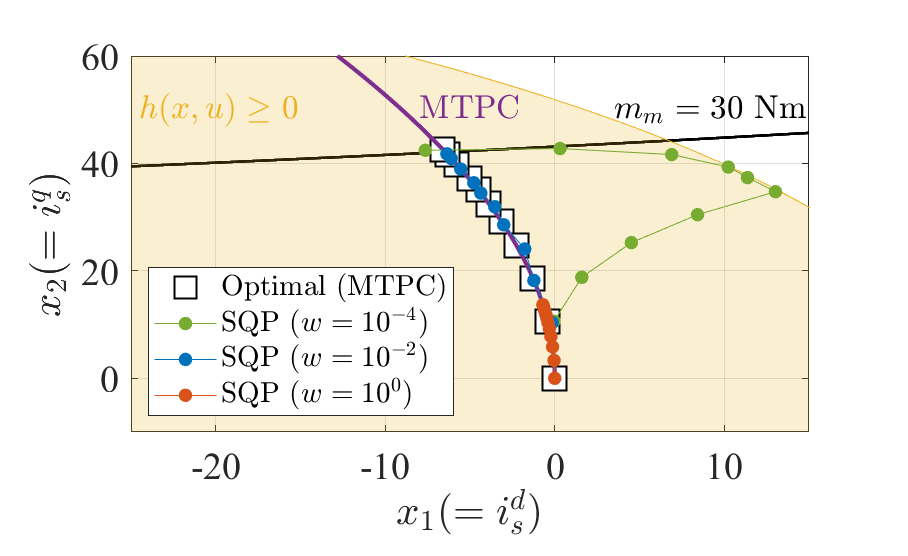
\includegraphics[width=0.85\linewidth]{Fig_SQP_MTPA}%
\label{Fig_SQP_MTPA}}
\vfill
\subfigure[]{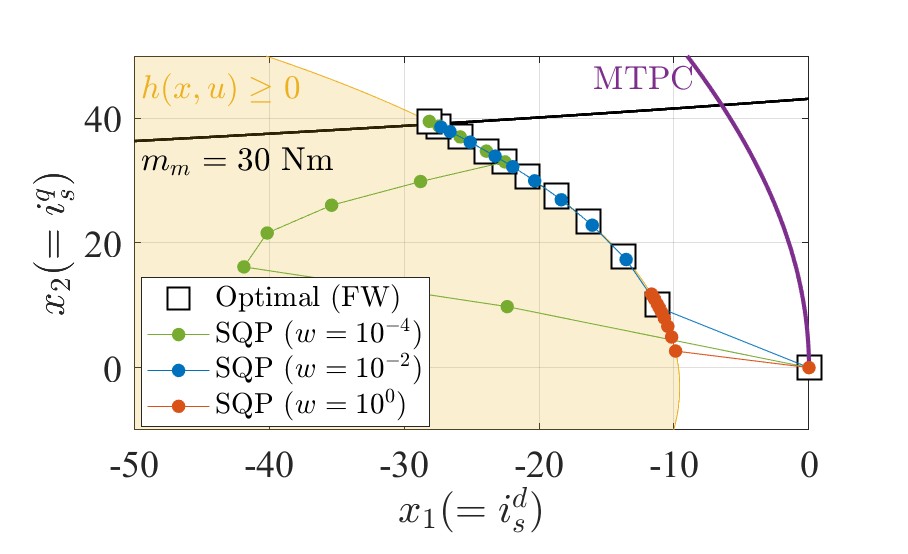
\includegraphics[width=0.85\linewidth]{Fig_SQP_FW}%
\label{Fig_SQP_FW}}
\caption{NMPC results obtained using SQP with $w = 10^{-4}, 10^{-2},$ and $10^{0}$ for the conditions of (a) $w_r = 840$ rad/s  and (b) $w_r = 1090$ rad/s.
}\label{Fig_SQP}
\end{figure}

\begin{figure}%[!b]
\centering
\subfigure[]{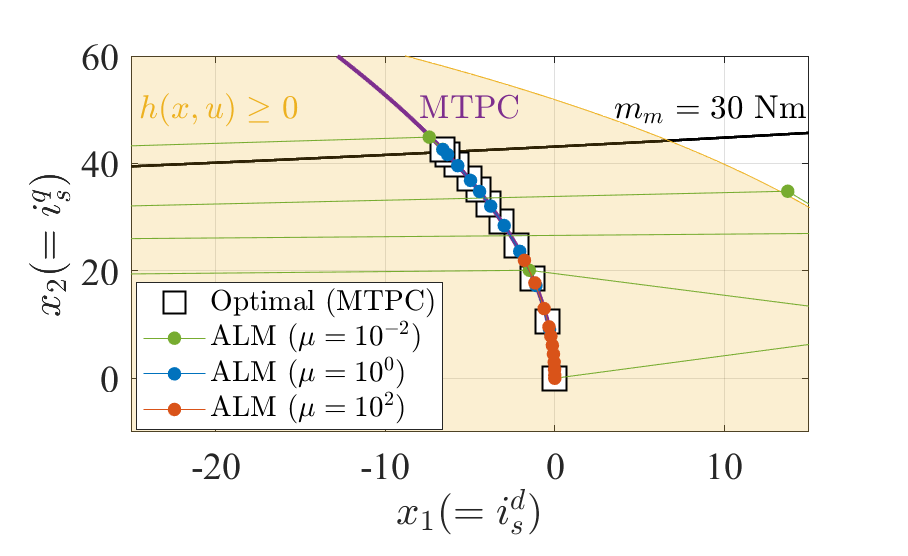
\includegraphics[width=0.85\linewidth]{Fig_ALM_MTPA}%
\label{Fig_ALM_MTPA}}
\vfill
\subfigure[]{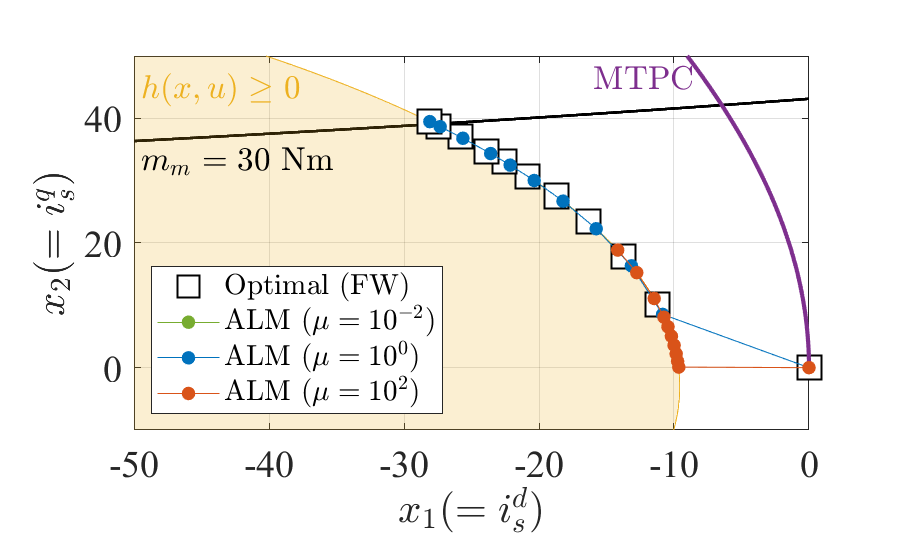
\includegraphics[width=0.85\linewidth]{Fig_ALM_FW}%
\label{Fig_ALM_FW}}
\caption{NMPC results obtained using ALM with $\mu = 10^{-2}, 10^{0},$ and $10^{2}$ for the conditions of (a) $w_r = 840$ rad/s  and (b) $w_r = 1090$ rad/s.
}\label{Fig_ALM}
\end{figure}

The NMPTC results obtained using SQP with $w = 10^{-4}, 10^{-2},$ and $10^{0}$ are shown in Fig. \ref{Fig_SQP}. $x_1$ and $x_2$ on the horizontal and vertical axes represent the first and second elements of the state $\mv{x}$, respectively. The MTPA line, denoted by dashed lines in the figures, represents the points satisfying
\begin{subequations}
\begin{align}
&\mathop {\min }\limits_x q(x,u)\\\nonumber
&{\rm{subject\ to}}\\
&e = r - y = 0,
\end{align}
\end{subequations}
meaning the target points of the state $\mv{x}$ when the inequality constraint $h(x,u) \ge 0$ is inactive. with $w = 10^{-4}$, the state trajectory, $x_t$, satisfied the tracking condition $e_{t+N} = 0$ well but quite deviated from the control-effort-minimizing points (i.e., MTPA line) due to the large portion of the tracking error terms (see Fig. \ref{Fig_SQP}). with $w = 10^{0}$, the state trajectory aligned with the MTPA line when the inequality constraint was inactive (see Fig. \ref{Fig_SQP_MTPA}) or moved close to the MTPA line even when the constraint was active (see Fig. \ref{Fig_SQP_FW}). However, the state trajectory hardly satisfied the tracking condition due to the large portion of the control effort term. The balance between the tracking error terms and control effort term was made with $w = 10^{-2}$.

The NMPTC results obtained using ALM with $\mu = 10^{-2}, 10^{0},$ and $10^{2}$ are shown in Fig. \ref{Fig_ALM}. with $\mu = 10^{-2}$, the state trajectory, $x_t$, was unstable until reaching the final point when the inequality constraint was inactive (see Fig. \ref{Fig_ALM_MTPA}). This was because the barrier parameter $\mu$ was too small so the Lagrange multiplier for the inequality constraint (\ref{eq:NMPC2_3}) was easily updated and considered active, which had to be inactive.
% Fig. 4b에 대한 언급도 필요?
with $w = 10^{2}$, by contrast, the state trajectory hardly satisfied the tracking condition because the Lagrange multiplier for the equality constraint (\ref{eq:NMPC2_5}) was updated slowly due to the large value of $\mu$. The Lagrange multipliers for the constraints were updated appropriately with $\mu = 10^{0}$, and thus a desirable state trajectory was obtained.

The NMPTC results obtained using update laws 1 and 2 (i.e., LBNLP) of repeating the for-loop once and twice are shown in Figs. \ref{Fig_UL1} and \ref{Fig_LBNLP}, respectively. While update law 1 showed good convergence with only one iteration when the inequality constraint is not active, update law 1 failed to handle the active constraint with one iteration (see Fig. \ref{Fig_UL1_FW}). Update law 1 with two iterations converged to the target point at the end; however, it showed an infeasible transient behavior (i.e., the inequality constraint was violated) (see. Fig (\ref{Fig_UL1_FW}). On the other hand, LBNLP provided an almost direct move to the target points even with one repetition of the for-loop (see Fig. \ref{Fig_LBNLP}). Just one more repetition of the for-loop guaranteed a very accurate move. This result is significant in that conventional methods like SQP and ALM provided satisfactory results only with appropriate values of tuning parameters, 
% Tuning parameter에 대한 sensitivity
whereas LBNLP guaranteed a desirable result just by repeating the simple algorithm once or twice, not relying on tuning parameters.

\KYCH{Computation times will be replaced by a table or just text data, considering the page limit.}
Computation times of representative results of each method are shown in Fig. \ref{Fig9}. The representative results were selected as Figs. \ref{Fig2b}, \ref{Fig5b}, and \ref{Fig7b} for SQP, ALM, and the proposed method, respectively. The computation times of SQP were approximately one hundred times greater than those of ALM and the proposed method, which is probably due to the inversion of the KKT matrix for SQP and multiple iterations to elaborate solutions. The average computation time of ALM was approximately twice greater than that of the proposed method. This is because ALM used multiple iterations to guarantee the convergence of Newton's method. This result verifies that the proposed method, which is matrix-inversion-free and does not require large numbers of iterations, is computationally efficient.


\section{Conclusion}

This study presented a novel numerical optimization method to solve NLP. This method was designed based on a Lyapunov approach to reach the necessary conditions for optimality. The advantage of using the Lyapunov approach was the update law was derived in a tuning-parameter-free and matrix-inversion-free manner; thus, the proposed method could be implemented easily with less iteration and computation time than conventional methods, such as SQP and ALM. The effectiveness of the proposed method was validated by using it to solve an NLP problem, which was an NMPC problem for optimal torque control of PMSMs, and comparing it with SQP and ALM.

The following issues need to be handled in a future study:
%\begin{itemize}
    %\item \textbf{Validation for large-scale problems:} This study used a small-scale NLP problem, whose number of optimization variables was two. The effectiveness of the proposed method is expected to be further highlighted for large-scale problems. A possible target problem would be an NMPC problem with a longer prediction horizon like the one presented in \cite{de2022system}.
    %\item \textbf{Proof of the convergence rate:} No discussion was made on the convergence rate of the proposed method. The convergence rate of the proposed method needs to be investigated in that other methods such as SQP guarantee quadratic convergence near local solutions. 
    %\item \textbf{Considerations on global convergence:} Ensuring global convergence is a very well-known but challenging issue in numerical optimization. Nonetheless, it is expected to guarantee global and fast convergence for an NMPC problem if a well-approximated problem is solved and the approximated solution is provided as the initial guess for the original problem. For instance, define the optimization variable as ${u_t} = {\hat u_t} + \Delta {u_t}$, where ${\hat u_t}$ is the solution of an approximated problem and $\Delta {u_t}$ is the deviation between the true and approximated solutions. The approximated solution ${\hat u_t}$ could be obtained by solving the following problem:
    %\begin{subequations}\label{eq:NMPC3}
    %\begin{align}
    %&\mathop {\min }\limits_{{u_t}} {{\hat q}\left( {{x_{t}},{u_{t}}} \right)} \\\nonumber
    %&{\rm{subject\ to}}\\
    %&{x_{t + 1}} = {\hat f}\left( {{x_{t}},{u_{t}}} \right),\ {y_{t}} = {\hat g}({x_{t}},{u_{t}}),\\
    %%&{\hat h}({x_{t + 1}},{u_{t + 1}}) \ge 0,\\
    %&{x_t} = x(t),\\
    %&{e_{t + 1}} = 0,
    %\end{align}
    %\end{subequations}
    %where the prediction horizon $N$ is set to 1, $\hat q$ is a quadratic approximation of function $q$, and, $\hat f$ and $\hat g$ are linear approximations of function $f$ and $g$, respectively. This is a QP with equality constraints, whose solution is easily obtained by solving a KKT matrix. Then, the original problem (\ref{eq:NMPC2}) is rewritten with the new optimization variable $\Delta {u_t}$ and solved by the proposed method.
    %\end{itemize}


\CHHA{In the figures, the correct operation strategy should be indicated as well; at the moment, the reader might think that MTPA should work but all methods do not always converge to the MTPA hyperbola (of course, this is due to the voltage constraint, Hence, we should show FW, MTPV, etc. all "correct" points on the operation strategy line. }\KYCH{I will add such indications in the next update of the figures.} \CHHA{I would present for both angular velocities all results of SQP, ALM and LBNLP in ONE FIG. It would be nice if the simulations could show ALL OFTC operation strategies such as MPTC, MC, FW, MTPV - do you think this is feasible?}


\begin{figure}[!t]
\centering
\subfigure[]{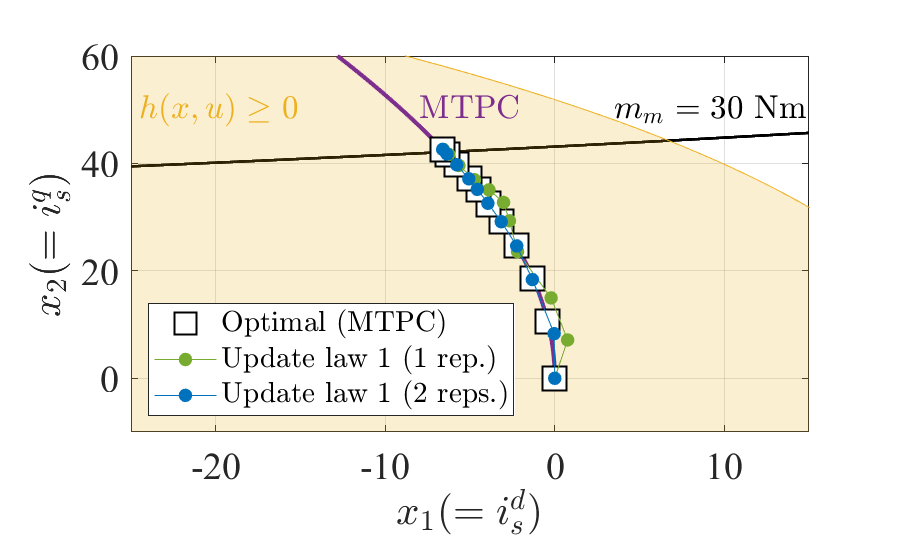
\includegraphics[width=0.88\linewidth]{Fig_UL1_MTPA}%
\label{Fig_UL1_MTPA}}
\vfill
\subfigure[]{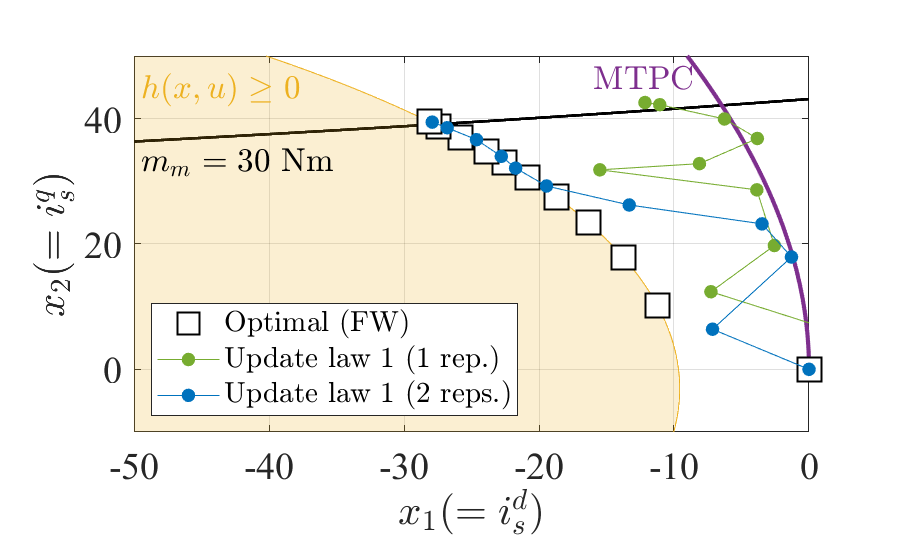
\includegraphics[width=0.88\linewidth]{Fig_UL1_FW}%
\label{Fig_UL1_FW}}
\caption{NMPC results obtained using update law 1 of repeating the for-loop once and twice for each time instant $t$, for the conditions of (a) $w_r = 840$ rad/s  and (b) $w_r = 1090$ rad/s.
}\label{Fig_UL1}
\end{figure}

\begin{figure}[!t]
\centering
\subfigure[]{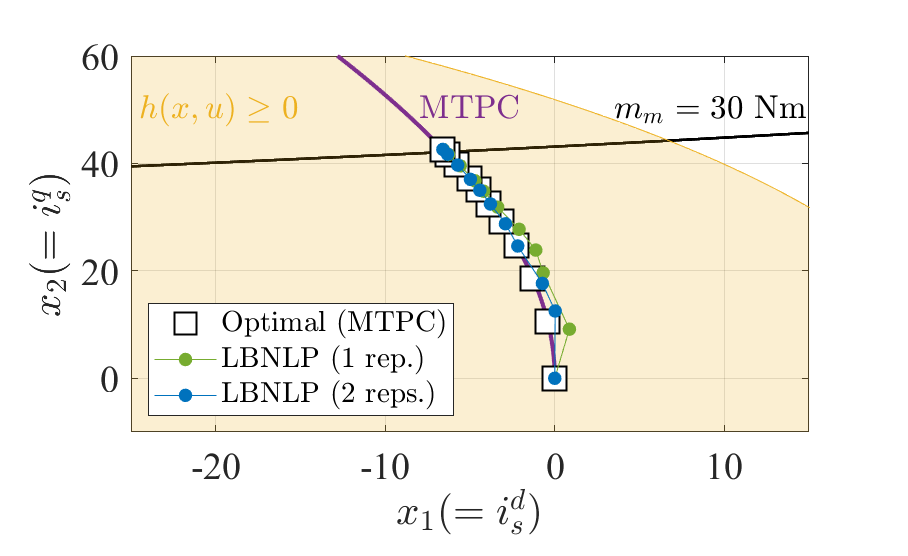
\includegraphics[width=0.88\linewidth]{Fig_LBNLP_MTPA}%
\label{Fig_LBNLP_MTPA}}
\vfill
\subfigure[]{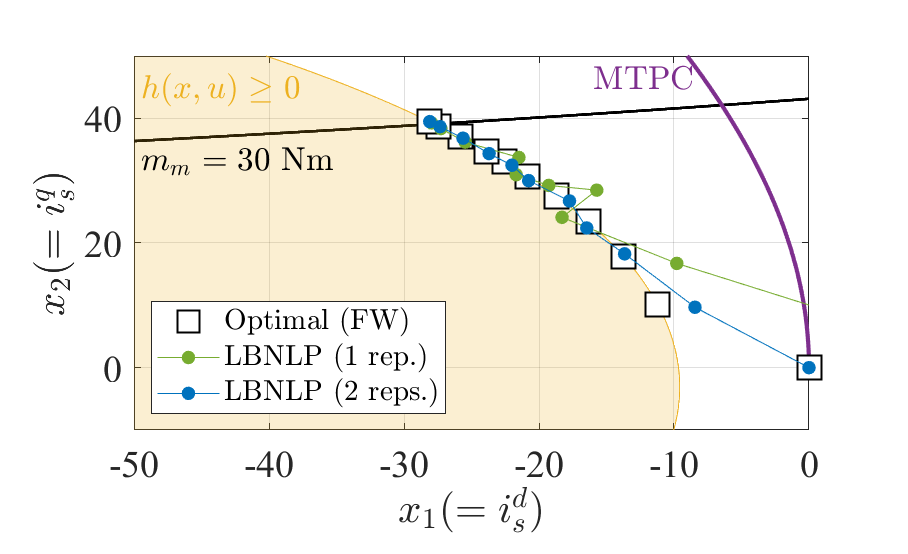
\includegraphics[width=0.88\linewidth]{Fig_LBNLP_FW}%
\label{Fig_LBNLP_FW}}
\caption{NMPC results obtained using LBNLP (update law 2) of repeating the for-loop once and twice for each time instant $t$, for the conditions of (a) $w_r = 840$ rad/s  and (b) $w_r = 1090$ rad/s.
}\label{Fig_LBNLP}
\end{figure}


%\begin{figure}[!t]
%\centering
%\subfigure[]{\includegraphics[width=0.9\linewidth]{Fig9a}%
%\label{Fig9a}}
%\vfill
%\subfigure[]{\includegraphics[width=0.9\linewidth]{Fig9b}%
%\label{Fig9b}}
%\vfill
%\subfigure[]{\includegraphics[width=0.9\linewidth]{Fig9c}%
%\label{Fig9c}}
%\caption{Computation time at each time instant $t$ of (a) the SQP's result presented in Fig. \ref{Fig2b}, (b) the ALM's result presented in Fig. \ref{Fig5b}, and (c) update law 3's result presented in Fig. \ref{Fig7b}. The solid lines and shaded areas represent the mean values and standard deviations, respectively. \KYCH{The title of Fig. 9(c) will be revised as update law 3.}
%}\label{Fig9}
%\end{figure}

%\clearpage


%\section*{Appendix}
%Appendixes, if needed, appear before the acknowledgment.

%\section*{Acknowledgment}
%The preferred spelling of the word ``acknowledgment'' in American English is without an ``e'' after the ``g.'' Use the singular heading even if you have many acknowledgments. Avoid expressions such as ``One of us (S.B.A.) would like to thank ... .'' Instead, write ``F. A. Author thanks ... .'' In most cases, sponsor and financial support acknowledgments are placed in the unnumbered footnote on the first page, not here.



% References
\bibliographystyle{Bibliography/IEEEtranTIE}
\bibliography{Bibliography/IEEEabrv,Bibliography/BIB_xx-TIE-xxxx,Bibliography/LMRES_Bibliography}\ %IEEEabrv instead of IEEEfull

	
%\vspace{-1cm}
% \begin{IEEEbiography}[{
\includegraphics[width=1in,height=1.25in,clip,keepaspectratio]{photo-men.eps}}]
% {First A. Author1} and the other authors may include biographies at the end of regular papers. The first paragraph may contain a place and/or date of birth (list place, then date). Next, the author's educational background is listed. The degrees should be listed with type of degree in what field, which institution, city, state or country, and year degree was earned. The author's major field of study should be lower-cased.

% The second paragraph uses the pronoun of the person (he or she) and not the author's last name. It lists military and work experience, including summer and fellowship jobs. Job titles are capitalized. The current job must have a location; previous positions may be listed without one. Information concerning previous publications may be included.

% The third paragraph begins with the author's title and last name (e.g., Dr. Smith, Prof. Jones, Mr. Kajor, Ms. Hunter). List any memberships in professional societies other than the IEEE. Finally, list any awards and work for IEEE committees and publications. If a photograph is provided, the biography will be indented around it. The photograph is placed at the top left of the biography. Personal hobbies will be deleted from the biography.
% \end{IEEEbiography}

% %\vspace{-1cm}
% \begin{IEEEbiography}[{
\includegraphics[width=1in,height=1.25in,clip,keepaspectratio]{photo-men.eps}}]
% {Second B. Author2} (M'12) was born in City, Country. He received the M. degree in electrical engineering from University of City, Country in 2012.

% The second paragraph uses the pronoun of the person (he or she) and not the author's last name. It lists military and work experience, including similar information to the previous author, including military, work experience, and other jobs. Job titles are capitalized. The current job must have a location; previous positions may be listed without one. Information concerning previous publications may be included.

% The third paragraph begins with the author's title and last name (e.g., Dr. Smith, Prof. Jones, Mr. Kajor, Ms. Hunter), including similar information to the previous author, including the list of any awards and work for IEEE committees and publications. The photograph is placed at the top left of the biography. Personal hobbies will be deleted from the 
% biography.
% \end{IEEEbiography}

% %\vspace{-2cm}
% \begin{IEEEbiography}[{
\includegraphics[width=1in,height=1.25in,clip,keepaspectratio]{photo-men.eps}}]
% {Third C. Author3} (M'99-SM'04-F'09) was born in City, Country. He received the M. and SM. and F. degrees in electrical engineering from University of City, Country in 1999, 2004 and 2009 respectively.

% The second paragraph uses the pronoun of the person (he or she) and not the author's last name. It lists military and work experience, including similar information to the previous author, including military, work experience, and other jobs.

% The third paragraph begins with the author's title and last name (e.g., Dr. Smith, Prof. Jones, Mr. Kajor, Ms. Hunter), including similar information to the previous author, including the list of any awards and work for IEEE committees and publications. The photograph is placed at the top left of the biography. Personal hobbies will be deleted from the biography.
% %\\ \\ 
% \end{IEEEbiography}


\end{document}
